\documentclass[12pt, a4paper, oneside]{Thesis} % Paper size, default font size and one-sided paper
\usepackage[utf8]{inputenc}
\usepackage{wrapfig, float, bm}
\usepackage{lscape}
\usepackage{rotating}
%\usepackage{subcaption}
\usepackage[]{graphicx}
\usepackage{caption}
\usepackage{amsmath, nccmath}
\usepackage{comment}
\usepackage{afterpage}
\usepackage{multirow}
\usepackage{multicol}
\usepackage{cleveref}
\usepackage{rotating}
% \usepackage[font=small]{caption}
% \captionsetup{compatibility=false}
% \usepackage{subcaption}
% \usepackage{subfig}
\usepackage{makecell}
\usepackage{booktabs}
\usepackage{lscape}
\usepackage{longtable}
\usepackage{placeins}
\usepackage{adjustbox}
\usepackage{arydshln} % dashed midline
\usepackage{ragged2e}
\usepackage{lipsum}
\usepackage{mathtools} % To use box inside an aligned environment
\usepackage{enumitem} % for roman letter lists
\usepackage{setspace}
\usepackage{hyperref}
\usepackage{tabularx}
\newcommand\myemptypage{
    \null
    \thispagestyle{empty}
    \addtocounter{page}{-1}
    \newpage
    }
%\usepackage[width=14cm, left=3cm]{geometry}
%\usepackage[left=0.75in, right=0.75in, top=1in, bottom=1in]{geometry}


\renewcommand{\ttitle}{Cross-Lingual Representations and Mechanisms in Multilingual LLMs during Reinforcement Learning}
\newcommand{\tdate}{June 29, 2026}

% prints author names as small caps
\usepackage{amsmath, amssymb, amsfonts}
\usepackage{algorithm}
\usepackage{algpseudocode}   % for the algorithmic environment
\usepackage{booktabs}        % for the tables in this and the neuron chapter

%\usepackage{subcaption} %incompatible with subfig
\graphicspath{{Pictures/}} % Specifies the directory where pictures are stored
\usepackage[authoryear]{natbib}
\setcitestyle{square}
%\usepackage[square, numbers]{natbib} % Use the natbib reference package - read up on this to edit the reference style; if you want text (e.g. Smith et al., 2012) for the in-text references (instead of numbers), remove 'numbers' v
%\bibliographystyle{abbrvnat}
%\setcitestyle{authoryear,open={((},close={))}}
\hypersetup{urlcolor=blue, colorlinks=true} % Colors hyperlinks in blue - change to black if annoyingv`	
\title{\ttitle} % Defines the thesis title - don't touch this




%%%% New added


\usepackage{tikz}
\usetikzlibrary{shapes.geometric, arrows}

% Defining Tickz Style
\tikzstyle{startstop} = [rectangle, rounded corners, minimum width=3cm, minimum height=1cm, text centered, text width = 10cm, draw=black, fill=white]

% \tikzstyle{startstop1} = [rectangle, rounded corners, minimum width=3cm, minimum height=1cm, text centered, draw=black, fill=white, text width = 10cm]

% \tikzstyle{io} = [trapezium, trapezium left angle=70, trapezium right angle=110, minimum width=3cm, minimum height=1cm, text centered, text width = 4.5cm, draw=black, fill=blue!30]

\tikzstyle{process} = [rectangle, minimum width=3cm, minimum height=1cm, text centered, text width = 6cm, draw=black, fill=white, text width = 10cm]

% \tikzstyle{decision} = [diamond, minimum width=3cm, minimum height=1cm, text centered, draw=black, fill=green!30]

\tikzstyle{arrow} = [ultra thick,->,>=stealth, line width=0.7mm]







\usepackage[T1]{fontenc}
% ============================================================
% macros.tex -- shared math macros for the thesis
% % ============================================================
% macros.tex -- shared math macros for the thesis
% % ============================================================
% macros.tex -- shared math macros for the thesis
% \input{macros} in main.tex, before \begin{document}
	% ============================================================
	
	% ---- Math operators and sets ----
	\newcommand{\E}{\mathbb{E}}
	\newcommand{\R}{\mathbb{R}}
	\DeclareMathOperator*{\argmax}{arg\,max}
	\DeclareMathOperator*{\argmin}{arg\,min}
	
	% ---- FairPO notation ----
	\newcommand{\dataset}{\mathcal{D}}
	\newcommand{\labels}{\mathcal{T}}                              % set of all T labels
	\newcommand{\privileged}{\mathcal{P}}                          % privileged label set
	\newcommand{\nonprivileged}{\bar{\mathcal{P}}}                 % non-privileged label set
	\newcommand{\confusing}{S_{il}}                                % confusing set for (i,l)
	\newcommand{\model}{m}                                         % model score function
	\newcommand{\params}{\mathbf{w}}                               % model parameters
	\newcommand{\Params}{\{\mathbf{w}_t \vert t \in \mathcal{T}\}} % all model parameters
	\newcommand{\refparams}{\hat{\mathbf{w}}}                      % reference parameters
	\newcommand{\Refparams}{\{\hat{\mathbf{w}}_t \vert t \in \mathcal{T}\}} % all reference parameters
	\newcommand{\loss}{\mathcal{L}}
	\newcommand{\baseloss}{\ell}                                   % base loss (BCE) in main.tex, before \begin{document}
	% ============================================================
	
	% ---- Math operators and sets ----
	\newcommand{\E}{\mathbb{E}}
	\newcommand{\R}{\mathbb{R}}
	\DeclareMathOperator*{\argmax}{arg\,max}
	\DeclareMathOperator*{\argmin}{arg\,min}
	
	% ---- FairPO notation ----
	\newcommand{\dataset}{\mathcal{D}}
	\newcommand{\labels}{\mathcal{T}}                              % set of all T labels
	\newcommand{\privileged}{\mathcal{P}}                          % privileged label set
	\newcommand{\nonprivileged}{\bar{\mathcal{P}}}                 % non-privileged label set
	\newcommand{\confusing}{S_{il}}                                % confusing set for (i,l)
	\newcommand{\model}{m}                                         % model score function
	\newcommand{\params}{\mathbf{w}}                               % model parameters
	\newcommand{\Params}{\{\mathbf{w}_t \vert t \in \mathcal{T}\}} % all model parameters
	\newcommand{\refparams}{\hat{\mathbf{w}}}                      % reference parameters
	\newcommand{\Refparams}{\{\hat{\mathbf{w}}_t \vert t \in \mathcal{T}\}} % all reference parameters
	\newcommand{\loss}{\mathcal{L}}
	\newcommand{\baseloss}{\ell}                                   % base loss (BCE) in main.tex, before \begin{document}
	% ============================================================
	
	% ---- Math operators and sets ----
	\newcommand{\E}{\mathbb{E}}
	\newcommand{\R}{\mathbb{R}}
	\DeclareMathOperator*{\argmax}{arg\,max}
	\DeclareMathOperator*{\argmin}{arg\,min}
	
	% ---- FairPO notation ----
	\newcommand{\dataset}{\mathcal{D}}
	\newcommand{\labels}{\mathcal{T}}                              % set of all T labels
	\newcommand{\privileged}{\mathcal{P}}                          % privileged label set
	\newcommand{\nonprivileged}{\bar{\mathcal{P}}}                 % non-privileged label set
	\newcommand{\confusing}{S_{il}}                                % confusing set for (i,l)
	\newcommand{\model}{m}                                         % model score function
	\newcommand{\params}{\mathbf{w}}                               % model parameters
	\newcommand{\Params}{\{\mathbf{w}_t \vert t \in \mathcal{T}\}} % all model parameters
	\newcommand{\refparams}{\hat{\mathbf{w}}}                      % reference parameters
	\newcommand{\Refparams}{\{\hat{\mathbf{w}}_t \vert t \in \mathcal{T}\}} % all reference parameters
	\newcommand{\loss}{\mathcal{L}}
	\newcommand{\baseloss}{\ell}                                   % base loss (BCE)

\begin{document}
% \makeatletter
% \renewcommand*{\NAT@nmfmt}[1]{\textsc{#1}}
% \makeatother

% prints author names as small caps
% it is sometimes necessary in user documents to have access to such package-internal macros, and so the commands \makeatletter and \makeatother change the catcode 

\fancypagestyle{plain}{
	\fancyhf{}
	\cfoot{\thepage}
	\renewcommand{\headrulewidth}{0pt}
}

\frontmatter % Use roman page numbering style (i, ii, iii, iv...) for the pre-content pages

\setstretch{1.6} % Line spacing of 1.6 (double line spacing)

% Define the page headers using the FancyHdr package and set up for one-sided printing
\fancyhead{} % Clears all page headers and footers
\rhead{\thepage} % Sets the right side header to show the page number
\lhead{} % Clears the left side page header

\pagestyle{fancy} % Finally, use the "fancy" page style to implement the FancyHdr headers

\newcommand{\HRule}{\rule{\linewidth}{0.5mm}} % New command to make the lines in the title page

% PDF meta-data
\hypersetup{pdftitle={\ttitle}}
\hypersetup{pdfsubject=\subjectname}
\hypersetup{pdfauthor=\authornames}
\hypersetup{pdfkeywords=\keywordnames}




% --------------------------------------------------





%----------------------------------------------------------------------------------------
%	TITLE PAGE
%----------------------------------------------------------------------------------------
\begin{comment}
\begin{titlepage}
\begin{center}

\HRule \\[0.4cm] % Horizontal line
{\huge \bfseries \ttitle}\\[0.4cm] % Thesis title
\HRule \\[1.5cm] % Horizontal line
 
\large \textit{A thesis submitted in fulfillment of the requirements\\ for the degree of \degreename}\\[0.3cm] % University requirement text
\textit{by}\\[0.4cm]

%\href{http://home.iitk.ac.in/~saiwal}{\authornames}

\vfill
\graphicspath{ {./Figures/} }
\begin{figure}[hb]
  \centering
  \includegraphics[width=0.4\linewidth]{Images/redlogo.png}
\end{figure}

\DEPTNAME\\ % Research group name and department name
\textsc{ \UNIVNAME}\\[1.5cm] % University name
\large \today\\[2cm] % Date


\end{center}

\end{titlepage}
\end{comment}
%\begin{document}
%\begin{titlepage}


%\include{title1}
%\end{titlepage}
%\myemptypage
%\afterpage{\null\newpage}
%\include{blank_page_1}
%\newpage
%\newpage
%\newgeometry{centering,top = 2.54cm,bottom = 2.54cm,left = 2.54cm, right = 2.54cm, includeheadfoot}

\pagenumbering{gobble}% Remove page numbers (and reset to 1)
\thispagestyle{empty}
\singlespacing
\begin{titlepage}
%\setlength{\voffset}{-0.1in}
%\setlength{\headsep}{5pt}
%\setlength{\textheight}{650pt}
%titlepage
%\thispagestyle{empty}
\begin{center}
%\begin{minipage}{0.75\linewidth}
    \centering
     
%=====================================================%
%---------------THESIS TITLE--------------------------%
%=====================================================%    
\definecolor{blue}{rgb}{0,0,1} % before using a colour one has to define it like this, here you have given color with rgb as 0,0,1 as blue
      
  {{\Large \textbf{\ttitle}\par}}
%    \vspace{1cm}% FOR CREATING DESIRED SPACE BETWEEN THE LINES
     
%=====================================================%
%---------------Partial Fulfillment---------------------%
%=====================================================%
    \vspace{1cm}
    {Submitted in partial fulfilment of the requirements\\of the degree of \par}
    \vspace{0.1cm}
    {
    \textbf{\large Master of Science by Research} \par}
    \vspace{0.1cm}
    {in \par}
    \vspace{0.1cm}
    {\textbf{Data Science and Artificial Intelligence} \par}
    \vspace{0.1cm}

%=====================================================%
%---------------AUTHOR'S NAME-------------------------%
%=====================================================%
		
    {by\par}
    \vspace{0.1cm}
    {\large \textbf{\textcolor{blue}{Soumen Kumar Mondal}}\par} 
    (Roll No. 23m2157)
%    {\Large \textbf{(2013MEZ8469)}\par}
    \vspace{0.1cm}
    
%=====================================================%
%---------------Supervisor Name---------------------%
%=====================================================%    
%    {\Large \textbf{Doctor of Philosophy} \par}
%    \vspace{0.5cm}
    {Supervisor: \par}
    {\large \textbf{\textbf{\textcolor{blue}{Prof.~Preethi Jyothi}}}\par}
    (Associate Professor, CSE, IIT Bombay)
%    {\Large \textbf{(2013MEZ8469)}\par}
     \vspace{0.4 cm}

%=====================================================%
%---------------UNIVERSITY lOGO-----------------------%
%=====================================================%

\includegraphics[width=0.25\linewidth]{Images/iitb_logo.png}
%    \rule{0.4\linewidth}{0.15\linewidth}\par
     \vspace{0.4 cm}

    
%=====================================================%
%---------------DEPARTMENT'S NAME-------------------------%
%=====================================================%
    {\large Center for Machine Intelligence and Data Science (CMInDS)\par}

    {\large \textbf{INDIAN INSTITUTE OF TECHNOLOGY BOMBAY}\par}
%    \vspace{0.4cm}
%=====================================================%
%---------------DATE----------------------------------%
%=====================================================%
    {\large \textbf{Mumbai - 400076, India}}
%    \vspace{0.4cm}
    
    {\large {\tdate}}
%\end{minipage}
\end{center}
\end{titlepage}
\clearpage
\pagenumbering{roman}
\setcounter{page}{1}

\newpage
%\myemptypage

%----------------------------------------------------------------------------------------
%	DEDICATION
%----------------------------------------------------------------------------------------
%
\setstretch{1.3} % Return the line spacing back to 1.3

\pagestyle{empty} % Page style needs to be empty for this page

\dedicatory{\textit{Dedicated to my beloved parents.}} % Dedication text

\addtocontents{toc}{\vspace{2em}} % Add a gap in the Contents, for aesthetics
\newpage

%----------------------------------------------------------------------------------------
% Approval page
%----------------------------------------------------------------------------------------
\singlespacing
%\addtotoc{Approval}
%{\addtocontents{toc}{}
%
%\vspace{-1in}
%\begin{center}
%{\Large  {\bf BPS Approval}}
%\end{center}

\approval{\addtocontents{toc}{}

This thesis entitled \textbf{"\ttitle"} by \textbf{Soumen Kumar Mondal} is approved for the degree of \emph{Master of Science by Research in Data Science and Artificial Intelligence}.\\\\

\vspace{2cm}

\ldots\ldots \ldots\ldots \ldots\ldots \ldots\ldots \ldots\ldots  \hfill  \ldots\ldots \ldots\ldots \ldots\ldots \ldots\ldots \ldots\ldots \\
 \textbf{Prof.~Preethi Jyothi} \hfill \textbf{Prof.~Biplab Banerjee} \\
 Associate Professor, CSE, IIT Bombay \hfill  Associate Professor, CSRE, IIT Bombay \\
(Supervisor) \hfill (Internal Examiner)\\\\

\vspace{2cm}

\ldots\ldots \ldots\ldots \ldots\ldots \ldots\ldots \ldots\ldots  \hfill  \ldots\ldots \ldots\ldots \ldots\ldots \ldots\ldots \ldots\ldots \\
\textbf{Prof.~Name} \hfill \textbf{Prof.~Biplab Banerjee} \\
Designation, Dept, Institution \hfill  Associate Professor, CSRE, IIT Bombay \\
(External Examiner) \hfill (Chairman)\\\\

\vspace{2cm}

\noindent
Date: \tdate \\
Place: Mumbai, India

}

\newpage
%\myemptypage


%-------------------------------------------------------------
%	DECLARATION PAGE
%	Your institution may give you a different text to place here
%----------------------------------------------------------------------------------------

% ------------------------------------------------
% Professor's declaration

\certificate{\addtocontents{toc}{} % Add a gap in the Contents, for aesthetics

This is to certify that the thesis entitled \textbf{"\ttitle"}, submitted by \textbf{Soumen Kumar Mondal} to the Indian Institute of Technology Bombay, for the award of the degree of \emph{Master of Science by Research in Data Science and Artificial Intelligence}, is a record of the original, bona fide research work carried out by him under our supervision and guidance. The thesis has reached the standards fulfilling the requirements of the regulations related to the award of the degree.

\par The results contained in this thesis have not been submitted in part or in full to any other University or Institute for the award of any degree or diploma to the best of our knowledge.

\vspace{2cm}
\ldots\ldots \ldots\ldots \ldots\ldots \ldots\ldots \ldots\ldots \\
\textbf{Prof.~Preethi Jyothi}\\
Associate Professor, CSE, IIT Bombay \\
(Supervisor)

\vspace{2cm}

\noindent
Date: \tdate \\
Place: Mumbai, India


\vfill{}

}


\clearpage % Start a new page


% ------------------------------------------------
% Student declaration
%\singlespacing
%\addtotoc{Declaration} % Add the "Scope for future work" page entry to the Contents
%
%{\addtocontents{toc}{} % Add a gap in the Contents, for aesthetics
%
%\centerline{\textbf{\LARGE {Declaration}}}}
%\vspace{3em}
\declaration{\addtocontents{toc}{} % Add a gap in the Contents, for aesthetics

	
I declare that this written submission represents my ideas in my own words. Where others' ideas and words have been included, I have adequately cited and referenced the original source. I declare that I have adhered to all principles of academic honesty and integrity and have not misrepresented or fabricated, or falsified any idea/data/fact/source in my submission. I understand that any violation of the above will cause disciplinary action by the Institute and can also evoke penal action from the source which has thus not been properly cited or from whom proper permission has not been taken when needed. \\

\vspace{2cm}

\ldots\ldots \ldots\ldots \ldots\ldots \ldots\ldots \ldots\ldots \\
\textbf{Soumen Kumar Mondal}\\
Roll No. 23m2157

\vspace{2cm}

\noindent
Date: \tdate \\
Place: Mumbai, India

}

\clearpage % Start a new page
%\myemptypage



%----------------------------------------------------------------------------------------
%	CERTIFICATE OF COURSEWORK
%----------------------------------------------------------------------------------------
%\addtotoc{Certificate of Course Work}
%{\addtocontents{toc}{}
%
%\begin{center}
%    \large INDIAN INSTITUTE OF TECHNOLOGY BOMBAY, INDIA
%\end{center}
%
%\begin{center}
%    \textbf{CERTIFICATE OF COURSE WORK}
%\end{center}    
%
%\vspace{1cm}
%This is to certify that Student Name (Roll No. 16xxxxxxx) was admitted
%to the candidacy of Ph.D. degree on $30^{th}$ July 2023, after successfully completing all the courses required for the Ph.D. programme. The details of the course
%work done are given below.
%
%\vspace{1cm}
%
%\begin{center}
%\begin{tabular}{c c l c} 
% \toprule
% \textbf{Sl. No.} & \textbf{Course Code} & \textbf{Course Name} & \textbf{Credits} \\ [0.5ex] 
% \midrule
% 1 & CE740 & Traffic Engineering & 8 \\ 
% \midrule
% 2 & CE605 & Applied Statistics & 6 \\
% \midrule
% 3 & CE780 & Bhavioural Travel Modelling & 6 \\
% \midrule
% 4 & HS699 & Communication \& Presentation Skills & 4 \\
% \bottomrule
%\end{tabular}
%\end{center}
%
%\vspace{7cm}
%
%\begin{flushleft}
%IIT Bombay \\
%Date: \hfill Dy. Registrar (Academic)
%\end{flushleft}
%
%
%\clearpage % Start a new page
%
%\myemptypage


%----------------------------------------------------------------------------------------
%	ACKNOWLEDGEMENTS
%----------------------------------------------------------------------------------------

\singlespacing

\acknowledgements{\addtocontents{toc}{} % Add a gap in the Contents, for aesthetics

I take this opportunity to acknowledge and express my gratitude to my thesis supervisor \emph {Prof.~Preethi Jyothi} who supported and guided me during the research work. I am deeply thankful to the Almighty for the abundant grace and blessings that have allowed me to make significant progress on this project. \\

\vspace{2cm}

\textbf{Soumen Kumar Mondal}\\
Roll No. 23m2157

\vspace{2cm}

\noindent
Date: \tdate \\
Place: Mumbai, India

}
\clearpage % Start a new page

%\myemptypage



%----------------------------------------------------------------------------------------
%	ABSTRACT PAGE
%----------------------------------------------------------------------------------------

\addtotoc{Abstract} % Add the "Abstract" page entry to the Contents

\abstract{\addtocontents{toc}{} % Add a gap in the Contents, for aesthetics

Large language models acquire much of their behaviour from data and training
objectives whose effects are difficult to attribute to any single part of the
network. This thesis examines two settings where this difficulty is central. The
first concerns multilingual models and the extent to which their language
abilities can be tied to identifiable components or shaped by fine-tuning. The
second concerns preference-based optimization under competing objectives in
multi-label classification.

The first part asks whether language-specific neurons can be used to improve
cross-lingual transfer. Using activation-probability methods, we identify such
neurons in Llama 3.1 and Mistral Nemo and test interventions on them, both at
test time and through neuron-targeted LoRA fine-tuning, on XNLI and XQuAD. The
interventions yield negligible gains for low-resource languages. We also find
that setting activations to zero does not deactivate the neurons in any
meaningful sense, and that the neurons are not independent of one another. These
results suggest that language information is distributed across the network
rather than confined to a small, separable set of units.

The second part studies cross-lingual behaviour during reinforcement learning. We
fine-tune Qwen2.5-7B-Instruct on the MGSM benchmark with Group Relative Policy
Optimization and evaluate at regular checkpoints using accuracy, logit-lens
analysis across layers, and centred kernel alignment over residual
representations. The model predicts in English through the early and
middle layers and surfaces the target language only at the end, but this pattern
is present from the start and does not change over training, so the training does
not cause cross-lingual collapse. 

The third part addresses optimization under competing objectives in multi-label
classification. We propose FairPO, which splits labels into a privileged group,
optimized with a preference-based objective over confusing alternatives, and a
non-privileged group, kept near a reference model by a constrained objective. The
two objectives are balanced through a Group Robust Preference Optimization
formulation. On MS-COCO and NUS-WIDE, FairPO raises accuracy on rare labels while
leaving frequent labels largely unaffected.


}

\clearpage % Start a new page

%\myemptypage

%----------------------------------------------------------------------------------------
%	LIST OF CONTENTS/FIGURES/TABLES PAGES
%----------------------------------------------------------------------------------------

\pagestyle{fancy} % The page style headers have been "empty" all this time, now use the "fancy" headers as defined before to bring them back

\lhead{\emph{Contents}} % Set the left side page header to "Contents"
\tableofcontents % Write out the Table of Contents

\lhead{\emph{List of Figures}} % Set the left side page header to "List of Figures"
\listoffigures % Write out the List of Figures

\lhead{\emph{List of Tables}} % Set the left side page header to "List of Tables"
\listoftables % Write out the List of Tables
\lhead{\leftmark}
% ADD THIS after listoftables:

%----------------------------------------------------------------------------------------
%	ABBREVIATIONS
%----------------------------------------------------------------------------------------

%\clearpage % Start a new page
%
%\setstretch{1.25} % Set the line spacing to 1.5, this makes the following tables easier to read
%
%\lhead{\emph{Abbreviations}} % Set the left side page header to "Abbreviations"
%\listofsymbols{ll} % Include a list of Abbreviations (a table of two columns)
%{
%
%% \textbf{SM} & \textbf{S}afety \textbf{M}argin\\
%
%
%
%\textbf{AFT}  & \textbf{A}ccelerated  \textbf{F}ailure  \textbf{T}ime \\
%\textbf{ANOVA}  & \textbf{A}nalysis  \textbf{}of  \textbf{V}ariance\\
%\textbf{BLR}  & \textbf{B}inary \textbf{L}ogistic \textbf{R}egression\\
%
%}

%----------------------------------------------------------------------------------------

%----------------------------------------------------------------------------------------
%	SYMBOLS
%----------------------------------------------------------------------------------------

\clearpage % Start a new page

%\lhead{\emph{Symbols}} % Set the left side page header to "Symbols"
%
%\listofnomenclature{lll} % Include a list of Symbols (a two column table)
%{
%$\mu$ & Location parameter  \\
%$\lambda$ & Scale parameter  \\
%$\beta_0$ & Null model parameter  \\
%$\hat{\beta}$ & Fitted parameter  \\
%
%}



%----------------------------------------------------------------------------------------
%	THESIS CONTENT - CHAPTERS
%----------------------------------------------------------------------------------------

\mainmatter % Begin numeric (1,2,3...) page numbering

\pagestyle{fancy} % Return the page headers back to the "fancy" style


% Include the chapters of the thesis as separate files from the Chapters folder
% Uncomment the lines as you write the chapters

\chapter{Introduction}
\label{ch:introduction}

\section{Motivation}
\label{sec:intro-motivation}

Large language models perform well on many natural language tasks, but their
performance is not the same across languages. Models trained mostly on English and
a few other high-resource languages do worse on low-resource languages, even
though the same parameters are used for all of them
\citep{conneau2018xnli, shi2022mgsm}. A second issue is that it is hard to say
which part of a model is responsible for a given behaviour, and equally hard to
change that behaviour by editing a specific part. An intervention that looks
targeted often has little effect on the actual task.

Two lines of research address these issues from different directions. One studies
the model from the inside and asks where a capability is stored. Work on
language-specific neurons follows this direction, suggesting that a small set of
neurons accounts for much of how a model handles a particular language, and that
these neurons can be found from activation statistics
\citep{tang2024language, kojima2024multilingual}. The other line works through the
training objective, using preference-based and reinforcement-learning methods to
push model outputs towards a desired signal
\citep{rafailov2023direct, shao2024deepseekmath}. This thesis looks at both
directions together. The common observation across the studies reported here is
that editing a localized part of a model is often less useful than changing the
objective the model is trained on.

The problem matters for two reasons. In practice, low-resource languages and
imbalanced label sets are settings where data is limited, so a method that
actually moves a model's behaviour, rather than only appearing to, is worth
having. From a research point of view, the cases where an intervention fails are
informative: a neuron edit that changes nothing, or a training signal that moves a
representation without improving the task, tells us something about how these
models are organized.

\section{Problem Statement}
\label{sec:intro-problem}

This thesis studies the gap between what a model can do and what its training
makes it do, in two settings: cross-lingual learning in multilingual language
models, and optimization with competing objectives in multi-label classification.
We break this into three sub-problems.

\begin{enumerate}
	\item \textbf{Can localized internal components be used to control
		cross-lingual behaviour?} If language-specific neurons encode a language in a
	separable way \citep{tang2024language, kojima2024multilingual}, then editing
	them should improve performance on that language. The problem is to test this
	on downstream tasks, not only on language of generation, and to see whether
	the interventions give real gains.
	
	\item \textbf{How does reinforcement-learning fine-tuning change cross-lingual
		behaviour, and why does it help some languages but not others?} Training a
	multilingual model with a group-relative reinforcement objective
	\citep{shao2024deepseekmath} improves some languages and not others. The
	problem is to describe this difference and find the factor that controls it,
	rather than attributing it loosely to how low-resource a language is.
	
	\item \textbf{How can a model be improved on a chosen subset of labels without
		hurting the rest?} In multi-label classification, rare or important labels are
	not well served by a uniform loss, but improving them naively can degrade
	frequent labels. The problem is to design an objective that targets the chosen
	labels while protecting the others.
\end{enumerate}

\section{Research Questions}
\label{sec:intro-questions}

From these sub-problems, the thesis investigates the following questions.

\begin{itemize}
	\item \textbf{Are language-specific neurons useful for cross-lingual
		transfer?} Earlier work shows these neurons can control the \emph{language} a
	model generates in \citep{tang2024language, kojima2024multilingual}. It is not
	clear whether editing them improves performance on tasks such as natural
	language inference \citep{conneau2018xnli} and question answering
	\citep{artetxe2020cross} for low-resource languages.
	
	\item \textbf{Does a multilingual model process its reasoning in English at
		middle layers, and is that what holds back low-resource languages?} One
	hypothesis is that multilingual transformers work in an English-leaning space
	at middle layers \citep{wendler2024llamas}. We ask whether this holds during
	reinforcement-learning fine-tuning, and whether this or some other factor
	explains why certain languages do not improve.
	
	\item \textbf{Can preference optimization, which was developed for text
		generation, be used to manage competing objectives in a classification
		setting?} Methods such as DPO \citep{rafailov2023direct}, CPO
	\citep{xu2024contrastive}, and SimPO \citep{meng2024simpo} were built for
	generation. We ask whether their main ideas, together with a group-robust
	balancing method \citep{ramesh2024group}, can give targeted and fair
	improvements in multi-label classification.
\end{itemize}

\section{Research Details}
\label{sec:intro-details}

The thesis contains three studies, one for each question above. We describe them
briefly here and in full in the later chapters.

\subsection{Language-Specific Neurons and Cross-Lingual Transfer}
\label{sec:intro-neurons}

The first study, published at the Insights from Negative Results workshop at
NAACL~2025 \citep{mondal2025language}, tests whether language-specific neurons can
be used to improve cross-lingual transfer. We identify these neurons in Llama~3.1
and Mistral Nemo using Language Activation Probability Entropy and
activation-probability thresholding \citep{tang2024language}, and we try two kinds
of intervention: editing neuron activations at test time, and fine-tuning only
those neurons with a low-rank adapter \citep{hu2022lora}, on XNLI
\citep{conneau2018xnli} and XQuAD \citep{artetxe2020cross}. The interventions give
gains of less than one accuracy point on low-resource languages. We also find that
setting a neuron's activation to zero does not turn off the behaviour assigned to
it, and that the neurons found for different languages are not independent of one
another. These results do not support a clean, component-level account of how a
model handles language, and are consistent with a distributed encoding in which
single neurons carry more than one function \citep{elhage2022superposition}.

\subsection{Cross-Lingual Behaviour during Policy Optimization}
\label{sec:intro-grpo}

The second study looks at how cross-lingual behaviour changes during
reinforcement-learning fine-tuning, rather than in a fixed model. We fine-tune
Qwen2.5-7B-Instruct on the MGSM benchmark \citep{shi2022mgsm} using Group Relative
Policy Optimization \citep{shao2024deepseekmath} with a low-rank adapter, and we
measure the model at regular checkpoints. The measurements cover task accuracy,
the language of the model's intermediate predictions read off with the logit lens,
and the geometry of the residual-stream representations compared with centred
kernel alignment. Accuracy changes little across the seven languages over
training, and Telugu stays far below the rest throughout. Looking inside the
model, we find that it predicts in English through the early and middle layers and
surfaces the target language only in the last few layers, in line with the
latent-language hypothesis \citep{wendler2024llamas}. This pattern is already
present in the base model and does not change over training, so the fine-tuning
does not cause cross-lingual collapse. Telugu, the language that stays below the
rest, also has the fewest dedicated tokens in the Qwen2.5 tokeniser and is the one
whose representations change the most while its accuracy does not move. We trace
the per-language outcome to tokeniser coverage rather than to language identity:
when the vocabulary cannot represent a language at a fine enough level, the reward
signal is too coarse to give a useful gradient.

\subsection{Robust Preference Optimization for Multi-Label Classification}
\label{sec:intro-fairpo}

The third study, published at the OPT workshop at NeurIPS~2025
\citep{mondal2025fairpo}, uses preference optimization as a tool rather than as an
object of study. We propose FairPO, a method for multi-label classification that
splits the labels into a privileged group and a non-privileged group. The
privileged group is trained with a preference-based objective, adapted from DPO
\citep{rafailov2023direct}, CPO \citep{xu2024contrastive}, and SimPO
\citep{meng2024simpo}, that makes the model prefer a true label over the incorrect
labels most likely to be confused with it. The non-privileged group is kept close
to a reference model by a constrained objective, which prevents its performance
from dropping. The two objectives pull against each other, and we balance them
with a Group Robust Preference Optimization formulation \citep{ramesh2024group}
set up as a minimax problem over the groups. On MS-COCO and NUS-WIDE, FairPO
improves accuracy on rare privileged labels and leaves frequent labels almost
unchanged, doing better than the baselines we compare against.

We note one point about naming. Two different methods in this thesis share the
abbreviation GRPO. In Section~\ref{sec:intro-grpo} and
Chapter~\ref{ch:grpo-crosslingual}, GRPO means Group Relative Policy Optimization
\citep{shao2024deepseekmath}, a reinforcement-learning algorithm. In
Section~\ref{sec:intro-fairpo} and Chapter~\ref{ch:fairpo}, the balancing method
is Group Robust Preference Optimization \citep{ramesh2024group}, which comes from
the robust optimization literature. We write out the full name the first time it
appears in each chapter and do not use the abbreviation on its own to tell them
apart.

\section{Thesis Organization}
\label{sec:intro-organization}

The rest of the thesis is organized as follows.
Chapter~\ref{ch:related-work} reviews related work on multilingual
representations, language-specific neurons, preference optimization, and robust
optimization. Chapter~\ref{ch:neurons} presents the study of language-specific
neurons and cross-lingual transfer. Chapter~\ref{ch:grpo-crosslingual} presents
the study of cross-lingual behaviour during Group Relative Policy Optimization.
Chapter~\ref{ch:fairpo} presents FairPO and its results on multi-label
benchmarks. Chapter~\ref{ch:conclusion} summarizes the findings, states their
limitations, and describes directions for future work.
\chapter{Related Work}
\label{ch:related-work}

This chapter reviews prior work for the three studies in this thesis. We group it
into three sections. Section~\ref{sec:rw-neurons} covers language-specific neurons
and how earlier work has tried to use internal components to control multilingual
behaviour. Section~\ref{sec:rw-crosslingual} covers how multilingual models
process language across layers, and how this has been studied during and after
RL fine-tuning. Section~\ref{sec:rw-fairpo} covers multi-label
classification, preference optimization, and group-robust optimization, which are
the parts that FairPO builds on.

\section{Language-Specific Neurons and Internal Control of Multilingual Models}
\label{sec:rw-neurons}

\subsection{Identifying Language-Specific Neurons}
\label{sec:rw-neurons-id}

A line of work argues that a small number of neurons in a multilingual model are
responsible for handling a particular language. \citet{tang2024language} propose
Language Activation Probability Entropy (LAPE), which marks a neuron as
language-specific when it activates for one or a few languages and stays quiet for
the rest, and they show that these neurons sit mostly in the first and last layers
of the model. \citet{kojima2024multilingual} study decoder-based models and find
neurons that fire for a single language, with little overlap across languages.
Earlier work on encoder models reached a related conclusion:
\citet{durrani2020analyzing} show that small sets of neurons capture specific
linguistic properties, and \citet{bhattacharya2023unveiling} study language
specificity in the feed-forward layers of transformer models. These methods differ
in how they score and threshold neurons, but they share the assumption that
language is, at least in part, stored in identifiable units.

\subsection{Controlling and Editing Through Neurons}
\label{sec:rw-neurons-control}

Several papers go further and use these neurons to change model behaviour.
\citet{tang2024language} and \citet{kojima2024multilingual} show that turning
language-specific neurons on or off can steer the language a model generates in.
\citet{zhao2024multilingualism} detect language-specific neurons with a method
that needs no labelled data, and report that fine-tuning a small set of them
improves performance in a target language. Related ideas appear in machine
translation and style transfer: \citet{zhu2024landermt} route language-aware
neurons to reduce catastrophic forgetting during translation fine-tuning,
\citet{xie2021importance} allocate neurons between shared and language-specific
knowledge to improve translation, and \citet{lai2024style} steer text style by
turning off source-style neurons. Beyond language, \citet{huo2024mmneuron} study
domain-specific neurons in multimodal models and report accuracy gains from
manipulating them. \citet{zhang2024multilingual} edit factual knowledge across
languages using language-agnostic factual neurons.

\subsection{Limits of Neuron-Level Control}
\label{sec:rw-neurons-limits}

This control is not always reliable. A reason often given is that single neurons
do not correspond to single functions. \citet{elhage2022superposition} describe
superposition, where a neuron takes part in more than one feature, so editing it
affects several behaviours at once. Work that traces facts across languages also
suggests that knowledge is partly shared and partly transferred rather than stored
in separate per-language units \citep{zhao2024tracing}. Most of the steering
results above are reported on generation, that is, on which language the model
writes in, and not on whether the model answers a downstream task correctly. The
study in Chapter~\ref{ch:neurons} \citep{mondal2025language} works in this gap. It
tests whether neuron interventions help on XNLI \citep{conneau2018xnli} and XQuAD
\citep{artetxe2020cross} for low-resource languages, and finds that they do not,
that setting an activation to zero does not turn the neuron off, and that neurons
found for different languages are not independent.

\section{Cross-Lingual Processing in Language Models}
\label{sec:rw-crosslingual}

\subsection{The English-Centric View of Multilingual Processing}
\label{sec:rw-crosslingual-english}

A second group of papers studies how a multilingual model moves information across
its layers when given a non-English input. \citet{wendler2024llamas} track the
hidden states of Llama-2 on a word-translation task and describe three stages: the
hidden states start far from any output token, then pass through a region where
the model can already decode the answer but assigns more probability to its
English form, and finally move to a region specific to the input language. They
read this as evidence that the model works in a space closer to English at middle
layers. \citet{zhao2024multilingualism} propose a similar workflow, in which the
model understands the input, works in English in the middle layers, and produces
output in the target language at the end. \citet{lu2025paths} look at factual
recall and describe a pipeline in which the model uses an English-centric recall
mechanism and then translates the English answer back into the target language;
they point to two failure points, weak use of the English mechanism and wrong
translation back to the target, and propose vector interventions that improve
recall accuracy. Together these papers support the idea that English plays a
special role inside the model, but they study translation and factual recall in
fixed models rather than reasoning during training.

\subsection{Tools for Studying Internal Representations}
\label{sec:rw-crosslingual-tools}

The studies above rely on a few standard tools. The logit lens
\citep{nostalgebraist2020logitlens} reads out the model's prediction at each layer
by applying the output head to intermediate hidden states, which gives a
per-layer view of what the model would predict. To compare representations,
\citet{kornblith2019similarity} introduce Centered Kernel Alignment (CKA), a
similarity measure between two sets of representations that is invariant to
orthogonal transformations and isotropic scaling. CKA has been used to compare
representations across languages in multilingual models
\citep{conneau2020emerging}. The study in Chapter~\ref{ch:grpo-crosslingual} uses
both tools: the logit lens to check whether the model predicts in English at
middle layers, and CKA both across languages and across training checkpoints to
measure how much the representations move during fine-tuning.

\subsection{RL for Reasoning and Its Effect on Languages}
\label{sec:rw-crosslingual-rl}

Reinforcement learning is now a common way to improve reasoning in language
models. Group Relative Policy Optimization (GRPO) \citep{shao2024deepseekmath}
removes the separate value model used in PPO and instead estimates the baseline
from a group of sampled outputs for the same prompt. \citet{guo2025deepseekr1}
use GRPO to train a reasoning model with rewards based only on the correctness of
the final answer. Most of this work is evaluated on English or on a mixed set of
languages without separating the effect per language. Multilingual reasoning
itself is measured on benchmarks such as MGSM \citep{shi2022mgsm}, which
translates grade-school math problems into several languages. A separate line of
work shows that the cause of cross-lingual gaps can lie in the tokeniser:
\citet{petrov2023tokenizer} show that the same text can be split into very
different numbers of tokens across languages, which puts low-resource languages at
a disadvantage before the model runs. Chapter~\ref{ch:grpo-crosslingual} connects
these threads. It fine-tunes a multilingual model on MGSM with GRPO, checks the
English-centric processing claim during training, and finds that whether GRPO can
teach a language tracks tokeniser coverage rather than language identity.

\section{MLC and Preference Optimization}
\label{sec:rw-fairpo}

\subsection{Multi-Label Classification and Class Imbalance}
\label{sec:rw-fairpo-mlc}

Multi-label classification usually trains a model by minimizing an aggregate loss,
most often binary cross-entropy, over all labels at once. This treats every label
the same, which is a problem when some labels are rare or more important than
others. \citet{charte2015imbalance} study class imbalance in multi-label data and
the resampling methods used to address it. \citet{lin2018focal} propose Focal
Loss, which lowers the weight of easy examples so that training focuses on harder
ones, but it still scores each label on its own and does not compare a true label
against a specific competing one. Work on long-tailed multi-label recognition
\citep{guo2021longtailed} and on fairness in multi-label settings
\citep{liu2023simfair} addresses related problems, but does not target a chosen
subset of labels while protecting the rest. FairPO \citep{mondal2025fairpo}, the
study in Chapter~\ref{ch:fairpo}, fills this gap by splitting the labels into a
privileged group to improve and a non-privileged group to maintain. The standard
benchmarks here are MS-COCO \citep{lin2015coco} and NUS-WIDE
\citep{chua2009nuswide}, with a Vision Transformer backbone
\citep{dosovitskiy2021vit}, which FairPO also uses.

\subsection{Preference Optimization}
\label{sec:rw-fairpo-po}

Preference optimization was developed to align language models from preference
pairs. Direct Preference Optimization (DPO) \citep{rafailov2023direct} turns the
reinforcement-learning-from-human-feedback objective into a simple classification
loss over preferred and dispreferred outputs, without a separate reward model.
Several reference-free variants followed. Contrastive Preference Optimization
(CPO) \citep{xu2024contrastive} removes the reference model and adds a
negative-log-likelihood term to keep absolute quality. Simple Preference
Optimization (SimPO) \citep{meng2024simpo} uses the length-normalized average
log-probability as the implicit reward and adds a target margin. These methods
were built for text generation, where a preference is between two full sequences.
FairPO adapts their core idea, preferring a correct option over a confusing one,
to per-label scores in classification, so that the model is trained to score a
true label above the incorrect label most likely to be confused with it.

\subsection{Group-Robust Optimization}
\label{sec:rw-fairpo-dro}

The last component is the method used to balance the two groups. Distributionally
Robust Optimization, and in particular Group DRO \citep{sagawa2020dro}, minimizes
the worst-case loss over a set of predefined groups instead of the average loss,
which improves performance on the weakest group. Group Robust Preference
Optimization \citep{ramesh2024group} brings this idea to preference learning,
balancing performance across preference groups with adaptive weights in a minimax
setup. FairPO uses this formulation, but defines the groups by the label partition
rather than by preference source, and balances the preference-based loss for the
privileged group against the constrained loss for the non-privileged group. We
note again that this Group Robust Preference Optimization is a different method
from the Group Relative Policy Optimization of
Section~\ref{sec:rw-crosslingual-rl}, despite the shared abbreviation. 
\chapter{Language-Specific Neurons and Cross-Lingual Transfer}
\label{ch:neurons}

\section{Introduction}
\label{sec:neurons-intro}

\subsection{Motivation}
\label{subsec:neurons-motivation}

Multilingual models handle many languages with a single set of parameters, and one
open question is whether the information a model uses for a given language sits in
an identifiable part of the network. Work on language-specific neurons proposes
that it does. The claim is that a small number of neurons in the feed-forward
layers activate mainly for one language and stay quiet for others, and that these
neurons can be located from activation statistics
\citep{tang2024language, kojima2024multilingual}.

If this holds in a strong form, it points to a direct way to help low-resource
languages, where models tend to do worse than on high-resource ones. The idea would
be to find the neurons for a target language and change them, either at test time
or through fine-tuning, so that the model handles that language better. This is the
possibility we examine in this chapter.

Earlier work has shown that these neurons can control which language a model
generates text in. Turning them on or off pushes the model to produce output in a
given language or moves it away from that language
\citep{tang2024language, kojima2024multilingual}. This is a result about the
\emph{form} of the output, that is, the language the model writes in. It does not
say whether the neurons matter for the \emph{content} of a task, such as deciding
whether one sentence entails another or finding the answer to a question. Those
tasks need the model to use what it knows, not only to write in a particular
language. Whether language-specific neurons help on such tasks for low-resource
languages is the question we study here.

\subsection{Problem Statement}
\label{subsec:neurons-problem}

We study whether interventions on language-specific neurons improve cross-lingual
performance on downstream tasks. By cross-lingual transfer we mean the following
setting: the model is adapted using a source language, here English, for which
labelled data is available, and is then evaluated on a target language for which
we do not use task training data. If language-specific neurons carry the
information that lets the model handle a target language, then acting on those
neurons should raise target-language performance.

We make this concrete in two ways. First, we change the activations of the
identified neurons at test time, replacing them with statistical values computed
from a multilingual corpus, and measure the effect on the task. Second, we
fine-tune only the identified neurons with a low-rank adapter, so that the update
is restricted to those neurons, and again measure the effect. We run both kinds of
intervention on two tasks, natural language inference with XNLI
\citep{conneau2018xnli} and extractive question answering with XQuAD
\citep{artetxe2020cross}, using two models, Llama~3.1 \citep{grattafiori2024llama}
and Mistral Nemo \citep{mistral2024nemo}. We also compare two ways of identifying
the neurons, so that the conclusion does not depend on a single method.

\subsection{Contributions}
\label{subsec:neurons-contributions}

This chapter, based on our published work \citep{mondal2025language}, reports the
following.

\begin{itemize}
	\item We test two neuron identification methods, Language Activation
	Probability Entropy and activation-probability thresholding, on Llama~3.1 and
	Mistral Nemo, and two intervention types, test-time activation edits and
	neuron-targeted low-rank fine-tuning, on XNLI and XQuAD.
	
	\item We find that these interventions do not give consistent improvements on
	cross-lingual downstream tasks for low-resource languages. Where there is any
	gain it is small and not in a consistent direction, and several interventions
	degrade performance, sometimes sharply, more so for Mistral Nemo and on XQuAD.
	
	\item We report two further observations that explain the negative result.
	Setting a neuron's activation to zero does not remove its effect, which means
	zero is not a reliable way to turn a neuron off. And the neurons identified for
	different languages are not independent, so editing the neurons for one
	language affects others. These are consistent with neurons that take part in
	more than one function \citep{elhage2022superposition}.
\end{itemize}

The negative result here is the reason the rest of the thesis moves away from
editing internal components and towards methods that act on the training
objective.

\section{Background and Preliminaries}
\label{sec:neurons-background}

\subsection{Definition of a Neuron}
\label{subsec:neurons-definition}

We work with neurons in the feed-forward, or MLP, block of a transformer layer.
This subsection fixes what a neuron is so that the identification and intervention
methods later are precise.

Consider layer $i$ of a transformer. Let $H_{i-1} \in \mathbb{R}^{T \times d}$ be
the hidden states from the previous layer, where $T$ is the sequence length and
$d$ is the model dimension. The layer first applies multi-head self-attention. We
write its output as
\begin{equation}
	\hat{H}_i = \mathrm{Attn}\!\left(H_{i-1} W^i_q,\; H_{i-1} W^i_k,\; H_{i-1} W^i_v\right) W^i_o,
	\label{eq:neurons-attn}
\end{equation}
where $W^i_q, W^i_k, W^i_v, W^i_o \in \mathbb{R}^{d \times d}$ are the projection
matrices of the attention module and $\mathrm{Attn}(\cdot)$ is scaled dot-product
attention. The MLP block takes $\hat{H}_i$ as input.

In a standard transformer MLP, the block applies an up-projection, a non-linear
activation, and a down-projection:
\begin{equation}
	h_i = \mathrm{act\_fn}\!\left(\hat{H}_i W^i_1\right) W^i_2,
	\label{eq:neurons-mlp}
\end{equation}
where $W^i_1 \in \mathbb{R}^{d \times 4d}$ and $W^i_2 \in \mathbb{R}^{4d \times d}$
are the up- and down-projection matrices, and $\mathrm{act\_fn}(\cdot)$ is a
non-linear activation such as GELU or SiLU. The intermediate width is commonly
$4d$, though the exact factor depends on the model.

We define a neuron as one coordinate of the intermediate activation. The $j$-th
neuron of layer $i$ is
\begin{equation}
	h_{i,j} = \mathrm{act\_fn}\!\left(\left(\hat{H}_i W^i_1\right)_j\right),
	\label{eq:neurons-neuron}
\end{equation}
where $\left(\hat{H}_i W^i_1\right)_j$ is the pre-activation value of that neuron.
A neuron in this sense is a single hidden unit in the MLP, and its activation is a
scalar for each input token.

% FIGURE 3.1 -- include here.
% Suggested filename: fig_mlp_glu_architecture.pdf
% Content: schematic of the MLP/GLU block in a Llama-style layer, showing the
% self-attention output feeding the gate projection (W1), up projection (W3),
% the elementwise product after the SiLU activation, and the down projection (W2).
% Mark the j-th neuron on the intermediate (4d-wide) activation.
\begin{figure}[t]
	\centering
	 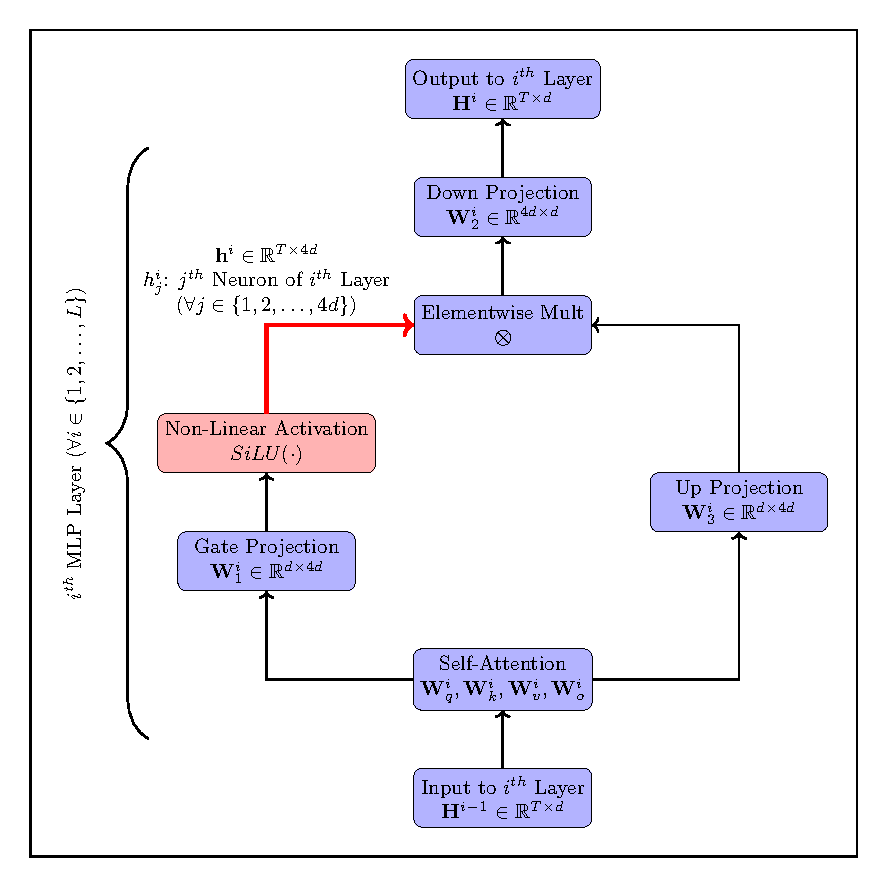
\includegraphics[width=0.8\linewidth]{Chapters/Chapter_3/mlp.pdf}
	\caption{Architecture of the MLP block in a Llama-style model. The output of
		self-attention is passed through a gate projection and an up projection, combined
		by an elementwise product after a SiLU activation, and then passed through a down
		projection. A neuron is one coordinate of the intermediate activation.}
	\label{fig:neurons-mlp-architecture}
\end{figure}

Recent models such as Llama use a gated variant of the MLP, the Gated Linear Unit
\citep{shazeer2020glu}. Here an extra projection $W^i_3$ gates the activation:
\begin{equation}
	h_i = \left[\mathrm{act\_fn}\!\left(\hat{H}_i W^i_1\right) \otimes \left(\hat{H}_i W^i_3\right)\right] W^i_2,
	\label{eq:neurons-glu}
\end{equation}
where $W^i_3 \in \mathbb{R}^{d \times 4d}$ and $\otimes$ is the elementwise
product. The gating lets the block represent richer transformations than the plain
MLP. The definition of a neuron does not change: it is still one coordinate of the
intermediate activation, now formed by the gated product.
Figure~\ref{fig:neurons-mlp-architecture} shows the block. Both models in this
chapter, Llama~3.1 and Mistral Nemo, use this gated form, so all neuron statistics
and interventions below act on the intermediate activations of
Equation~\ref{eq:neurons-glu}.

\subsection{Notation and Problem Setup}
\label{subsec:neurons-notation}

We collect the notation used in the rest of the chapter. A neuron is indexed by
its layer $i$ and position $j$ within that layer, written $(i,j)$. For an input
token at position $t$ in a sequence $s$, the activation of neuron $(i,j)$ is a
scalar, which we write $h^{(s,t)}_{i,j}$. We compute statistics of these
activations over a corpus, separately for each language, to decide which neurons
are specific to a language. The details of these statistics are in
Section~\ref{subsec:neurons-statistics}.

We consider a set of languages $L$. For a language $l \in L$, the identification
methods return a set of neurons $N_l$ that the method marks as specific to $l$. An
intervention is a change applied to the neurons in $N_l$, either replacing their
activations at test time or restricting fine-tuning to them. We evaluate the
effect of an intervention on a downstream task in a target language.

For the downstream tasks, we use a source language, English, for adaptation and a
target language for evaluation, and we do not use task training data in the target
language. This is the cross-lingual transfer setting described in
Section~\ref{subsec:neurons-problem}. The two tasks, XNLI and XQuAD, and their
evaluation metrics are defined in Section~\ref{sec:neurons-setup}.

\section{Identifying Language-Specific Neurons}
\label{sec:neurons-identify}

This section describes how we find the neurons that a method marks as specific to
a language. We first describe the corpus and the activation statistics we compute
from it (Section~\ref{subsec:neurons-statistics}), then the two identification
methods we use, Language Activation Probability Entropy
(Section~\ref{subsec:neurons-lape}) and activation-probability thresholding
(Section~\ref{subsec:neurons-actprob}), and finally the language sets we run them
on (Section~\ref{subsec:neurons-langsets}).

\subsection{Activation Statistics from a Multilingual Corpus}
\label{subsec:neurons-statistics}

To find language-specific neurons we first need a record of how each neuron
behaves on each language. We collect this from a multilingual corpus drawn from
Wikipedia \citep{wikidump}, using a subset of languages. Each language's text is
tokenized and passed through the model, and we record the activations from the MLP
modules.

Let $h^{t}_{i,j}$ be the activation of neuron $(i,j)$ at token position $t$ in a
sequence of length $T$. For a single sequence, the mean activation of the neuron
over its tokens is
\begin{equation}
	\bar{h}_{i,j} = \frac{1}{T} \sum_{t=1}^{T} h^{t}_{i,j}.
	\label{eq:neurons-seqmean}
\end{equation}
For a language $l$ with a set of sequences $\mathcal{S}_l$, we average over all
sequences to get a per-language profile of the neuron,
\begin{equation}
	h^{l}_{i,j} = \frac{1}{|\mathcal{S}_l|} \sum_{s \in \mathcal{S}_l} \bar{h}^{(s)}_{i,j}.
	\label{eq:neurons-langmean}
\end{equation}

Besides the mean, we compute the standard deviation and a set of quantiles of the
activations for each neuron and language, since some identification methods use
them. The $q$-quantile of a neuron's activation is
\begin{equation}
	P_q(h_{i,j}) = \inf\left\{ x \in \mathbb{R} : F_{h_{i,j}}(x) \geq q \right\},
	\label{eq:neurons-quantile}
\end{equation}
where $F_{h_{i,j}}$ is the cumulative distribution function of the neuron's
activations. We compute the 5th, 10th, 25th, 50th, 75th, 90th, and 95th
percentiles. These statistics, computed once per language, are the input to the
identification methods below and also to the test-time interventions in
Section~\ref{sec:neurons-intervene}.

\subsection{Language Activation Probability Entropy (LAPE)}
\label{subsec:neurons-lape}

The first method is Language Activation Probability Entropy (LAPE)
\citep{tang2024language}. The idea is that a neuron is specific to a language if it
tends to activate for that language and not for others. LAPE measures this with the
entropy of a neuron's activation probabilities across languages: a low entropy
means the neuron activates for one or a few languages, while a high entropy means
it activates evenly across all of them.

\paragraph{Step 1: Activation probabilities.}
For a language $l$, the activation probability of neuron $(i,j)$ is the fraction of
tokens for which the neuron has a positive activation,
\begin{equation}
	p^{l}_{i,j} = \mathbb{E}\left[ \mathbb{I}\!\left( h^{l}_{i,j} > 0 \right) \right],
	\label{eq:neurons-lape-prob}
\end{equation}
where $\mathbb{I}(\cdot)$ is the indicator function and the expectation is over all
tokens in all sequences for language $l$.

\paragraph{Step 2: Normalize across languages.}
For a set of $k$ languages, we normalize the probabilities so that they form a
distribution over languages for each neuron,
\begin{equation}
	\mathcal{P}^{l}_{i,j} = \frac{p^{l}_{i,j}}{\sum_{l'=1}^{k} p^{l'}_{i,j}}.
	\label{eq:neurons-lape-norm}
\end{equation}

\paragraph{Step 3: Entropy.}
The LAPE value of a neuron is the entropy of this distribution,
\begin{equation}
	\mathrm{LAPE}(i,j) = - \sum_{l=1}^{k} \mathcal{P}^{l}_{i,j} \log \mathcal{P}^{l}_{i,j}.
	\label{eq:neurons-lape-entropy}
\end{equation}
A small LAPE value marks a neuron that activates for few languages.
Figure~\ref{fig:neurons-lape-procedure} shows the steps.

% FIGURE 3.2 -- include here.
% Suggested filename: fig_lape_procedure.pdf
% Content: bottom-to-top flow for one neuron: per-language neuron activations ->
% unnormalized activation probabilities p^l_{i,j} -> normalized probabilities
% P^l_{i,j} -> LAPE entropy value. (This is the BPS1 LAPE figure.)
\begin{figure}[ht]
	\centering
	 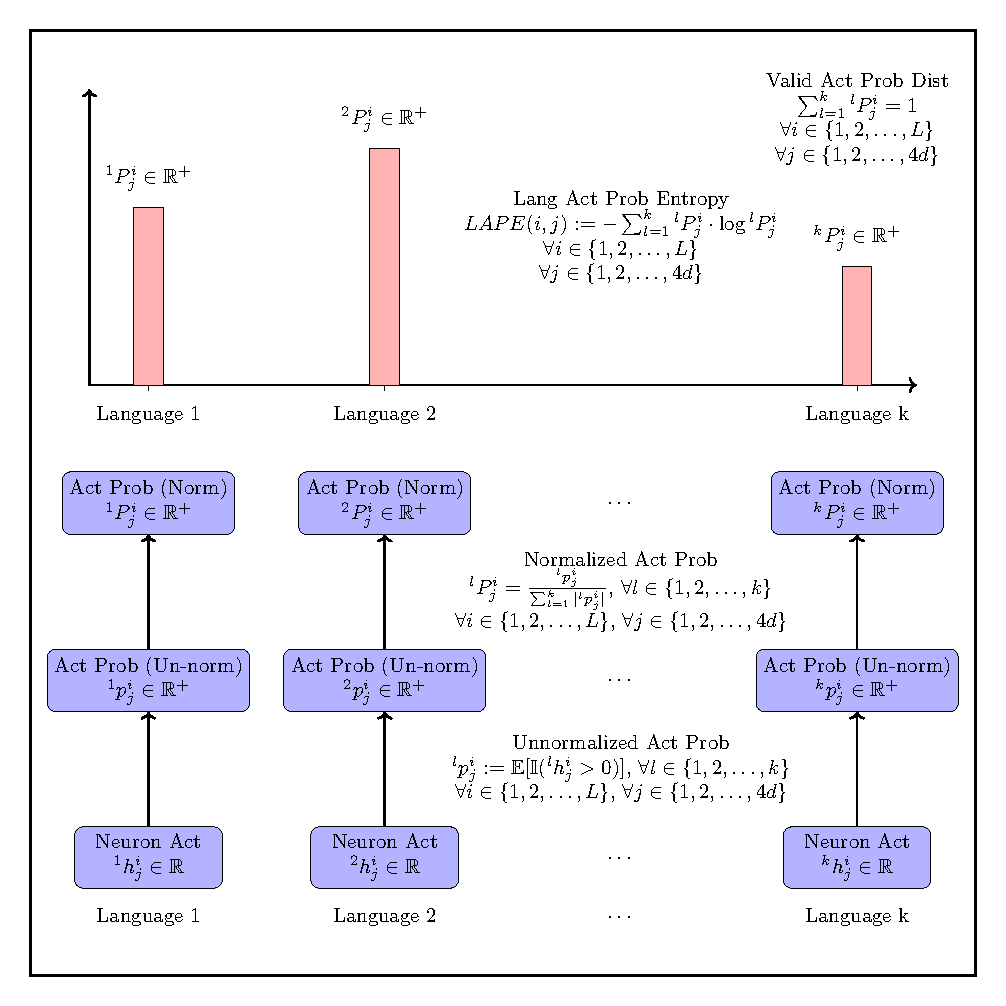
\includegraphics[width=0.8\linewidth]{Chapters/Chapter_3/lape.pdf}
	\caption{Computing LAPE for a single neuron. For each language we measure the
		probability that the neuron activates, normalize these probabilities across
		languages into a distribution, and take its entropy. Neurons with low entropy
		activate for only a few languages.}
	\label{fig:neurons-lape-procedure}
\end{figure}

\paragraph{Step 4: Threshold and selection.}
A neuron is only considered if it activates often enough for at least one language.
We set a threshold at the 95th percentile of the activation probabilities over all
neurons and languages,
\begin{equation}
	\mathrm{Threshold} = \mathrm{Quantile}_{0.95}\!\left( p_{i,j} \mid \forall i,j,l \right),
	\label{eq:neurons-lape-threshold}
\end{equation}
and keep neuron $(i,j)$ only if $p^{l}_{i,j} > \mathrm{Threshold}$ for some
language $l$. Among the neurons that pass, we select the ones with the lowest LAPE
values. We take the bottom $1\%$ of all neurons,
\begin{equation}
	m = \frac{1}{100} \times 4d \times L,
	\label{eq:neurons-lape-m}
\end{equation}
where $L$ is the number of layers and $4d$ the number of neurons per layer. Each
selected neuron is then assigned to the languages for which it activates above the
threshold, which gives the per-language neuron sets $N_l$.

\subsection{Activation-Probability Thresholding (Act Prob 90p)}
\label{subsec:neurons-actprob}

The second method scores each neuron by how often it activates strongly for a
language, and keeps the top-scoring neurons per language. We use this as a check
against LAPE, so that the conclusion does not rest on one identification method.
We refer to it as Act Prob 90p, after the relevance score we use.

\paragraph{Relevance score.}
For each neuron and language we compute a relevance value $r^{l}_{i,j}$. Several
choices are possible. The simplest is the activation probability, the fraction of
tokens with a positive activation,
\begin{equation}
	r^{l}_{i,j} = \mathbb{E}\left[ \mathbb{I}\!\left( h^{l}_{i,j} > 0 \right) \right].
	\label{eq:neurons-act-zero}
\end{equation}
We can also use the mean absolute activation, the probability of exceeding the
layer mean, or the probability of exceeding the 90th-percentile activation. The
last of these is the score we use in the main experiments,
\begin{equation}
	r^{l}_{i,j} = \mathbb{E}\left[ \mathbb{I}\!\left( h^{l}_{i,j} > P90^{l}_{i,j} \right) \right],
	\label{eq:neurons-act-90p}
\end{equation}
where $P90^{l}_{i,j}$ is the 90th percentile of the neuron's activations for
language $l$. This score picks out neurons that have rare but strong activations,
which we take as a sign of a specialized response.

\paragraph{Selection.}
For each language $l$ we collect the relevance values into a tensor
$R^{l} = \{ r^{l}_{i,j} \}$ and keep the top $m$ neurons by relevance. Here we use
\begin{equation}
	m = \frac{0.125}{100} \times L \times 4d,
	\label{eq:neurons-act-m}
\end{equation}
and the per-language set is
\begin{equation}
	N_l = \left\{ (i,j) \mid (i,j) \in \mathrm{Top}_m(R^{l}) \right\}.
	\label{eq:neurons-act-set}
\end{equation}
LAPE and Act Prob 90p differ in how they score and select neurons, so if both lead
to the same conclusion about interventions, the result is less likely to be an
artifact of one method.

\subsection{Language Sets}
\label{subsec:neurons-langsets}

We run the identification on two groups of languages, which we call Set1 and Set6.
Set1 is a mixed group covering several scripts and language families, used to study
neurons across languages that the model handles with varying success. Set6 is a
group of Indian languages, used to look more closely at the low-resource case that
is the focus of this chapter. Set1 covers English, French, Spanish, Vietnamese, Indonesian, Japanese, and Chinese, a mixed group across several scripts and families. Set6 covers English, Bengali, Hindi, Tamil, Telugu, Marathi, Urdu, Kannada, Malayalam, and Punjabi, the group of Indian
languages used to look more closely at the low-resource case. English is included
in both sets as the source language. We compute the activation statistics and run
both identification methods separately for each set, since the set of languages
changes the normalization in LAPE (Equation~\ref{eq:neurons-lape-norm}) and
therefore which neurons are selected.

\section{Intervening on Language-Specific Neurons}
\label{sec:neurons-intervene}

Having identified the neurons, we now change them and measure the effect. We use
two kinds of intervention. The first replaces neuron activations at test time
(Section~\ref{subsec:neurons-testtime}). The second fine-tunes only the identified
neurons (Section~\ref{subsec:neurons-lora}). We also describe a perplexity-based
probe (Section~\ref{subsec:neurons-ppxc}) that we use to check whether a test-time
intervention is doing anything to the model's handling of a language.

\subsection{Test-Time Interventions}
\label{subsec:neurons-testtime}

In a test-time intervention we run the model as usual, but for the neurons in
$N_l$ we replace the activation that the model would have produced with a fixed
value taken from the statistics in Section~\ref{subsec:neurons-statistics}. The
value is the same for every token, and the rest of the model runs unchanged. This
lets us ask whether forcing the language-specific neurons to a particular level
changes the model's behaviour on the target language.

We try several replacement values. The mean activation $\mu$ for the language sets
the neuron to its typical level. The higher percentiles, $P75$, $P90$, and $P95$,
push the neuron towards strong activation. The lower percentiles, $P25$, $P10$, and
$P5$, push it towards weak activation. We also try setting the activation to zero,
which is often described as turning the neuron off. As we show later
(Section~\ref{sec:neurons-results-transfer}), setting the activation to zero is not
the same as removing the neuron's effect, because zero is not a neutral value for
these activations.

\subsection{Perplexity Change as a Probe}
\label{subsec:neurons-ppxc}

Before measuring downstream task accuracy, it helps to check whether an
intervention affects the model's basic handling of a language at all. We use
perplexity for this. If the neurons in $N_l$ matter for language $l$, then
intervening on them should change the model's perplexity on text in language $l$.

We define the perplexity change $\mathrm{PPXC}(i,j)$ as the difference between the
perplexity on language $j$ after intervening on the neurons identified for language
$i$ and the perplexity with no intervention,
\begin{equation}
	\mathrm{PPXC}(i,j) = \mathrm{PPX}\!\left( j \mid \text{intervention on } i \right) - \mathrm{PPX}(j).
	\label{eq:neurons-ppxc}
\end{equation}
A value near zero means the intervention barely touches the model's handling of
language $j$. A large value means the intervention has a strong effect. Comparing
the diagonal entries ($i = j$, intervening on a language's own neurons) with the
off-diagonal entries ($i \neq j$, intervening with another language's neurons)
shows how specific the neurons are to their own language.

\subsection{Neuron-Targeted Fine-Tuning with LoRA}
\label{subsec:neurons-lora}

The second intervention fine-tunes the identified neurons rather than fixing their
activations. We use Low-Rank Adaptation (LoRA) \citep{hu2022lora}, which adds a
low-rank update $\Delta W$ to a weight matrix while leaving the pretrained weight
$W$ unchanged. The update is factored as
\begin{equation}
	\Delta W = A \cdot B,
	\label{eq:neurons-lora}
\end{equation}
with $A \in \mathbb{R}^{d_\text{in} \times r}$ and
$B \in \mathbb{R}^{r \times d_\text{out}}$, where the rank $r$ is much smaller than
$d_\text{in}$ or $d_\text{out}$.

To restrict the update to the identified neurons, we apply a binary mask to the
factors,
\begin{equation}
	A = \mathrm{mask}_A \cdot A_t, \qquad B = \mathrm{mask}_B \cdot B_t,
	\label{eq:neurons-lora-mask}
\end{equation}
where $A_t$ and $B_t$ are the trainable matrices. We leave $\mathrm{mask}_A$ all
ones, and in $\mathrm{mask}_B$ we set to zero the columns that correspond to
neurons we want to freeze. For a frozen neuron index $j_f$,
\begin{equation}
	[\mathrm{mask}_B]_{i,j} =
	\begin{cases}
		0, & \text{if } j = j_f, \; j_f \in \text{Frozen Neurons}, \\
		1, & \text{otherwise.}
	\end{cases}
	\label{eq:neurons-lora-maskb}
\end{equation}
This makes $\Delta W_{i,j} = 0$ for every frozen neuron, so no update reaches it.
The fine-tuned MLP output is then
\begin{equation}
	y = x \cdot W + x \cdot \Delta W,
	\label{eq:neurons-lora-out}
\end{equation}
where only the selected neurons receive an update through $\Delta W$.
Figure~\ref{fig:neurons-lora} illustrates the masking for a small example.

% FIGURE 3.3 -- include here.
% Suggested filename: fig_masked_lora.pdf
% Content: the BPS1 masked-LoRA diagram. Show DeltaW = A.B, the mask zeroing the
% columns of B for frozen neurons (e.g. neurons 3 and 5 frozen, LoRA rank 2),
% and the resulting DeltaW with zero columns at the frozen positions.
\begin{figure}[ht]
	\centering
	 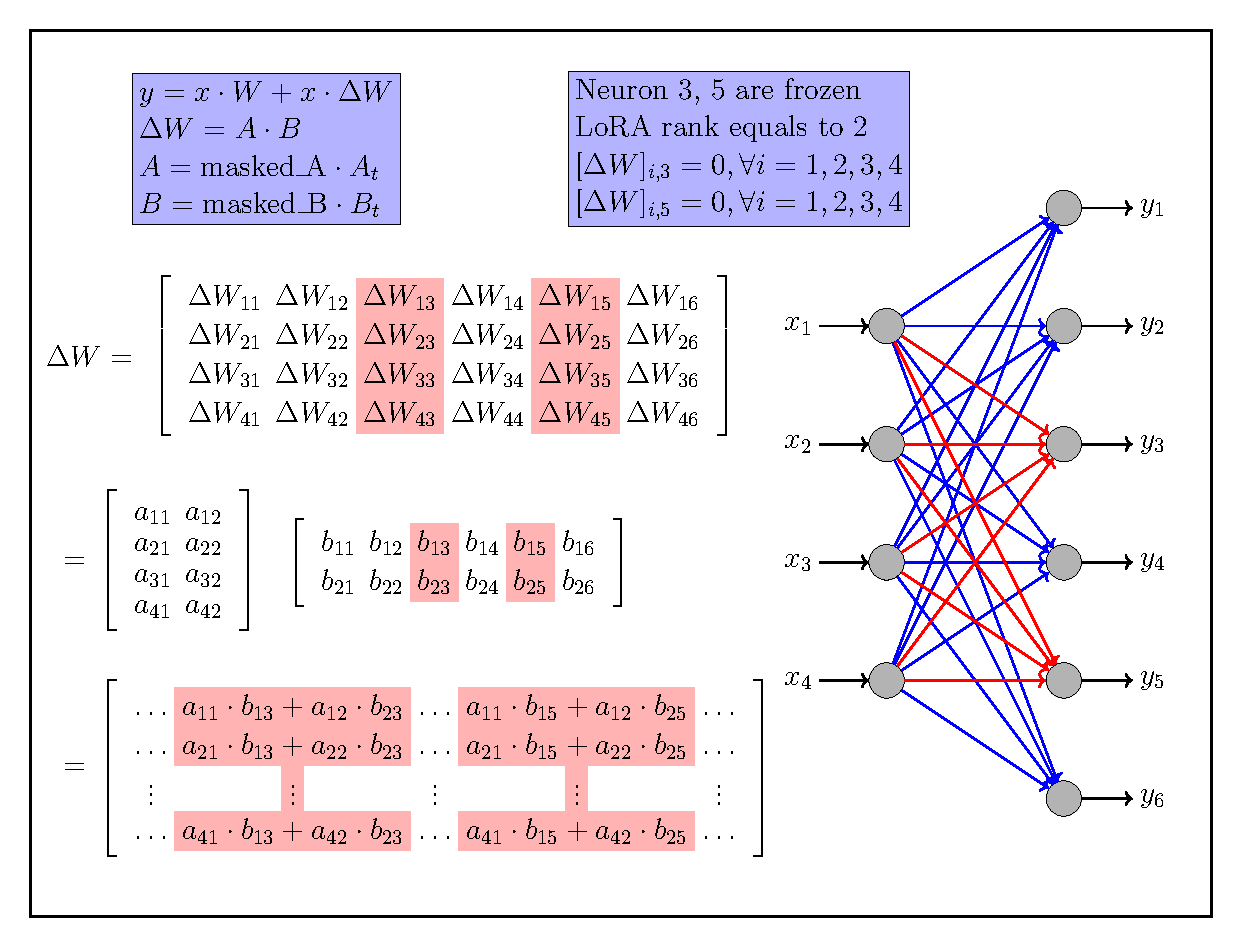
\includegraphics[width=0.8\linewidth]{Chapters/Chapter_3/lora.pdf}
	\caption{Neuron-targeted fine-tuning with masked LoRA. The low-rank update
		$\Delta W = A \cdot B$ is masked so that the columns of $B$ for frozen neurons
		are set to zero. In the example, neurons 3 and 5 are frozen with LoRA rank 2,
		so the corresponding columns of $\Delta W$ are zero and only the remaining
		neurons are updated.}
	\label{fig:neurons-lora}
\end{figure}

Alongside the masked MLP update, we always fine-tune the attention projections
($q$, $k$, $v$, $o$) and the task-specific head with ordinary LoRA. This keeps the
task performance reasonable, so that the comparison is between updating the
identified neurons and not updating them, rather than between training and not
training at all.

\subsection{Fine-Tuning Configurations}
\label{subsec:neurons-config}

We vary which language's neurons are fine-tuned. We refer to this as the
fine-tuning language (FTL). In one setting we fine-tune the neurons identified for
the source language, English. In another we fine-tune the neurons for the target
language. In a third we fine-tune the union of both. In all cases the task training
data is English, since we are testing cross-lingual transfer and do not use
target-language task data. Comparing these settings shows whether it matters which
language's neurons are made trainable, which is a direct test of whether the
language-specific sets carry transferable information.

\section{Experimental Setup}
\label{sec:neurons-setup}

\subsection{Models}
\label{subsec:neurons-models}

We use two pretrained multilingual models. Llama~3.1 \citep{grattafiori2024llama}
is an 8-billion-parameter model from Meta. Mistral Nemo \citep{mistral2024nemo} is
a 12-billion-parameter model. Both use the gated MLP of
Equation~\ref{eq:neurons-glu}, so the neuron definition and the identification
methods apply to both without change. We load both models in 4-bit precision to
reduce memory use.

\subsection{Tasks and Datasets}
\label{subsec:neurons-tasks}

\paragraph{XNLI.}
The Cross-lingual Natural Language Inference (XNLI) benchmark
\citep{conneau2018xnli} tests whether a model can decide the relationship between
two sentences across languages. Given a premise and a hypothesis, the model labels
the pair as entailment, neutral, or contradiction. We use English as the source
language and evaluate on lower-resource target languages from our language sets. We
form the input by joining the premise and hypothesis with a separator token and
tokenize to a maximum length of 512 tokens.

\paragraph{XQuAD.}
The Cross-lingual Question Answering Dataset (XQuAD) \citep{artetxe2020cross} tests
extractive question answering across languages. Given a passage and a question, the
model must select the span of the passage that answers the question. As with XNLI,
we adapt using English and evaluate on the target languages, without using
target-language task data.

\subsection{Implementation Details}
\label{subsec:neurons-impl}

For neuron identification we collect activations on the Wikipedia corpus
\citep{wikidump} with a maximum sequence length of 512 tokens. For fine-tuning we
use LoRA on the MLP neurons as described in
Section~\ref{subsec:neurons-lora}, together with LoRA on the attention projections
and the task head. We train with the AdamW optimizer and mixed-precision
computation. The full list of hyperparameters, including LoRA rank, scaling factor,
learning rate, number of epochs, and batch size for each task, is given in
Table~\ref{tab:neurons-hyperparams}.

\subsection{Evaluation Metrics}
\label{subsec:neurons-metrics}

For XNLI we report classification accuracy on the three-way label. For XQuAD we
report exact match and F1 between the predicted span and the reference answer. For
the neuron analysis we report the perplexity change $\mathrm{PPXC}$ of
Equation~\ref{eq:neurons-ppxc}, along with counts and overlaps of the identified
neurons. The no-intervention numbers in
Section~\ref{sec:neurons-results-transfer} serve as the baseline against which all
interventions are compared.

\section{Results: Neuron Analysis}
\label{sec:neurons-results-analysis}

Before looking at task performance, we study the neurons that the two methods
identify. This tells us how many neurons are marked per language, how much the
sets overlap across languages, where they sit in the model, and whether
intervening on them changes the model's handling of a language at all. We run this
analysis on the two language sets, Set1 and Set6, described in
Section~\ref{subsec:neurons-langsets}.

\subsection{Number of Language-Specific Neurons}
\label{subsec:neurons-counts}

Figure~\ref{fig:neurons-counts} shows the number of neurons identified per language
by LAPE, for both models on Set1 and Set6. The counts vary by language and are a
small fraction of the total number of neurons, as expected from the selection rule
in Equation~\ref{eq:neurons-lape-m}. The Act Prob 90p method works differently: by
construction it keeps a fixed number of top-scoring neurons per language
(Equation~\ref{eq:neurons-act-m}), which is $573$ per language for Llama~3.1 and
$717$ for Mistral Nemo, so its per-language counts are equal and we do not plot
them. Either way the identified set is small. This sets up the rest of the analysis:
the neurons are few enough that, if they carried language-specific function in a
clean way, intervening on them should be both possible and visible.

% FIGURE 3.4 -- include here.
% Suggested filename: fig_neuron_counts.pdf
% Content: bar charts of the number of language-specific neurons per language,
% LAPE vs Act Prob 90p, for Llama 3.1 and Mistral Nemo, on Set1 and Set6.
\begin{figure}[ht]
	\centering
	 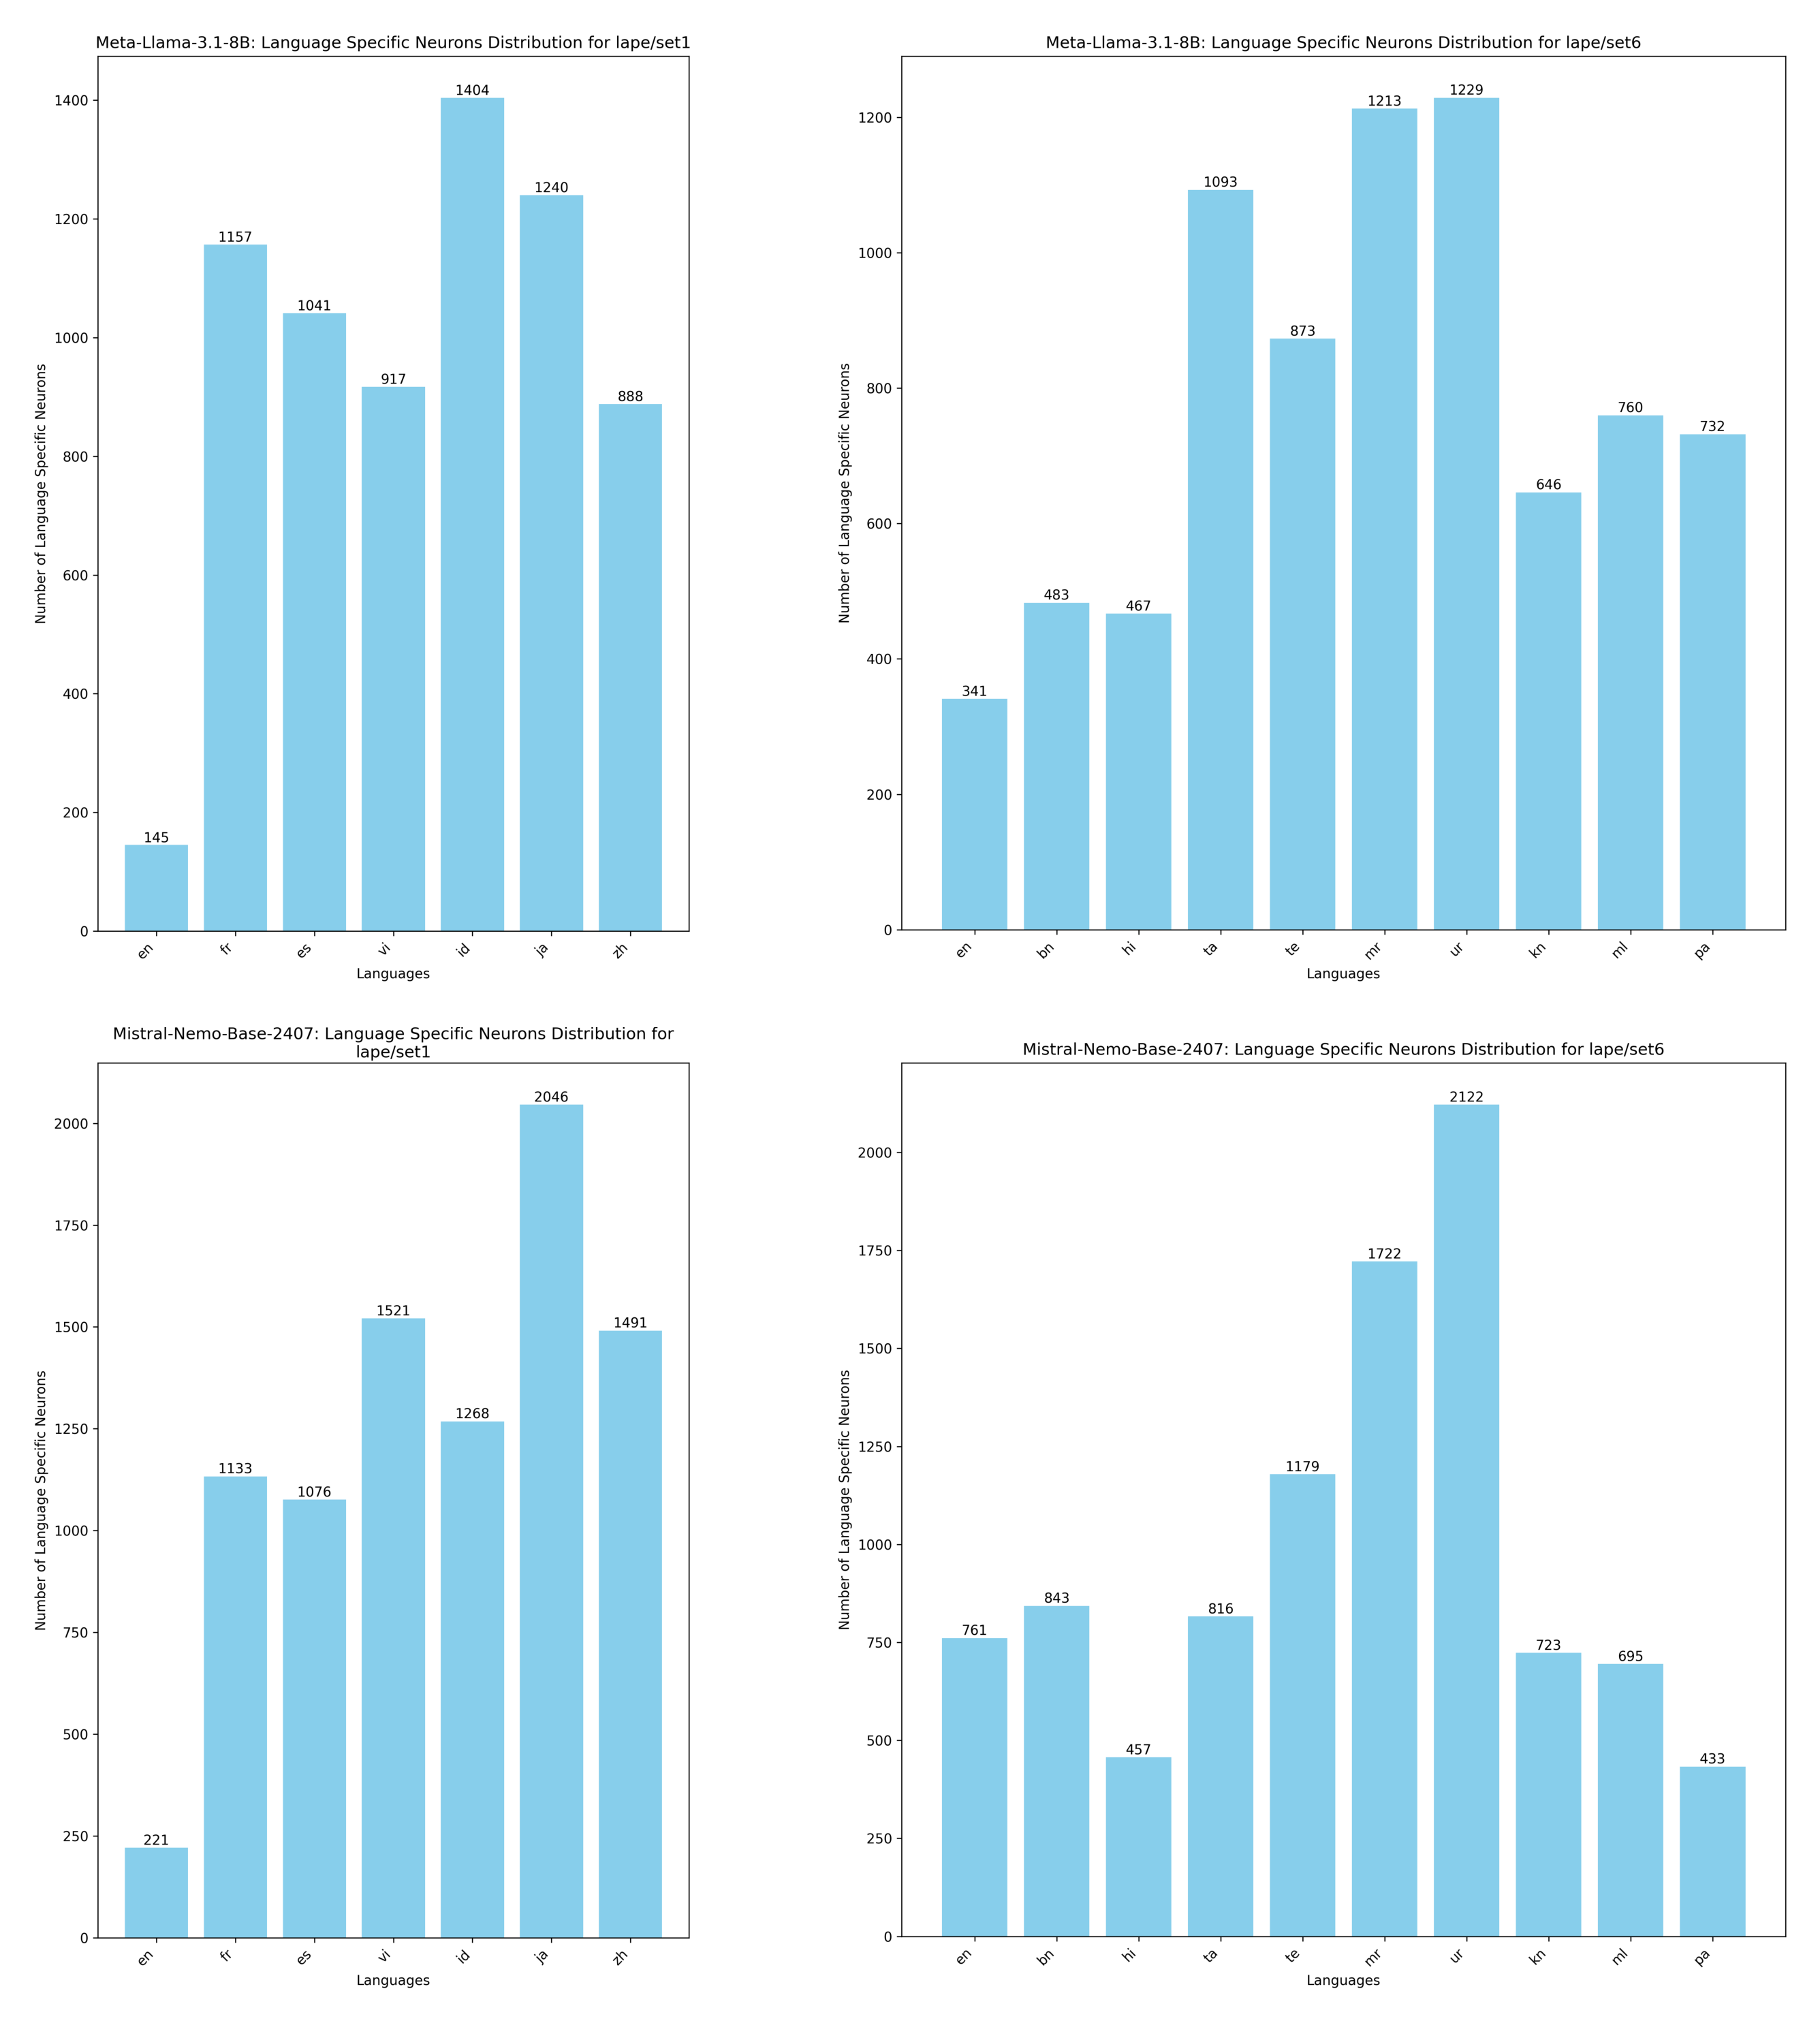
\includegraphics[width=0.8\linewidth]{Chapters/Chapter_3/figures/results/combined_lang_neuron_dist.png}
	\caption{Number of language-specific neurons identified per language by LAPE  for Llama~3.1 and Mistral Nemo on Set1 and Set6. Both models
		assign a small set of neurons to each language.}
	\label{fig:neurons-counts}
\end{figure}

\subsection{Overlap Between Languages}
\label{subsec:neurons-overlap}

If a neuron were specific to one language, it would appear in the set for that
language and no other. To check this, we count how many neurons are shared between
each pair of languages. Figure~\ref{fig:neurons-overlap-actprob} shows the overlap
for Act Prob 90p, and Figure~\ref{fig:neurons-overlap-lape} shows it for LAPE. In
each heatmap the diagonal is the size of a language's own set, and an off-diagonal
entry is the number of neurons two languages have in common.

The sets are far from disjoint. Under Act Prob 90p, where each language has 573
neurons in Llama~3.1 and 717 in Mistral Nemo, the shared counts between pairs of
languages often run to a few hundred, so a sizable part of any one set is not
unique to that language. LAPE shows the same thing on its larger sets. The amount
of sharing also tracks how close the languages are: pairs such as Japanese and
Chinese in Set1 overlap much more than unrelated pairs, and the Indian languages in
Set6 overlap most among themselves.

This is the first sign that the identified neurons are not cleanly tied to a single
language, and it matters for the interventions that follow. If a neuron belongs to
several languages at once, it cannot be changed for one of them without affecting
the others, so there is no clean way to act on a single target language through
these sets.

% FIGURE 3.5a (Act Prob 90p) -- include here.
% Suggested filename: fig_neuron_overlap_actprob.png
% Content: pairwise neuron-set overlap heatmaps for Act Prob 90p, for Llama 3.1 and
% Mistral Nemo (en, vi, ur, hi, zh).
\begin{figure}[ht]
	\centering
	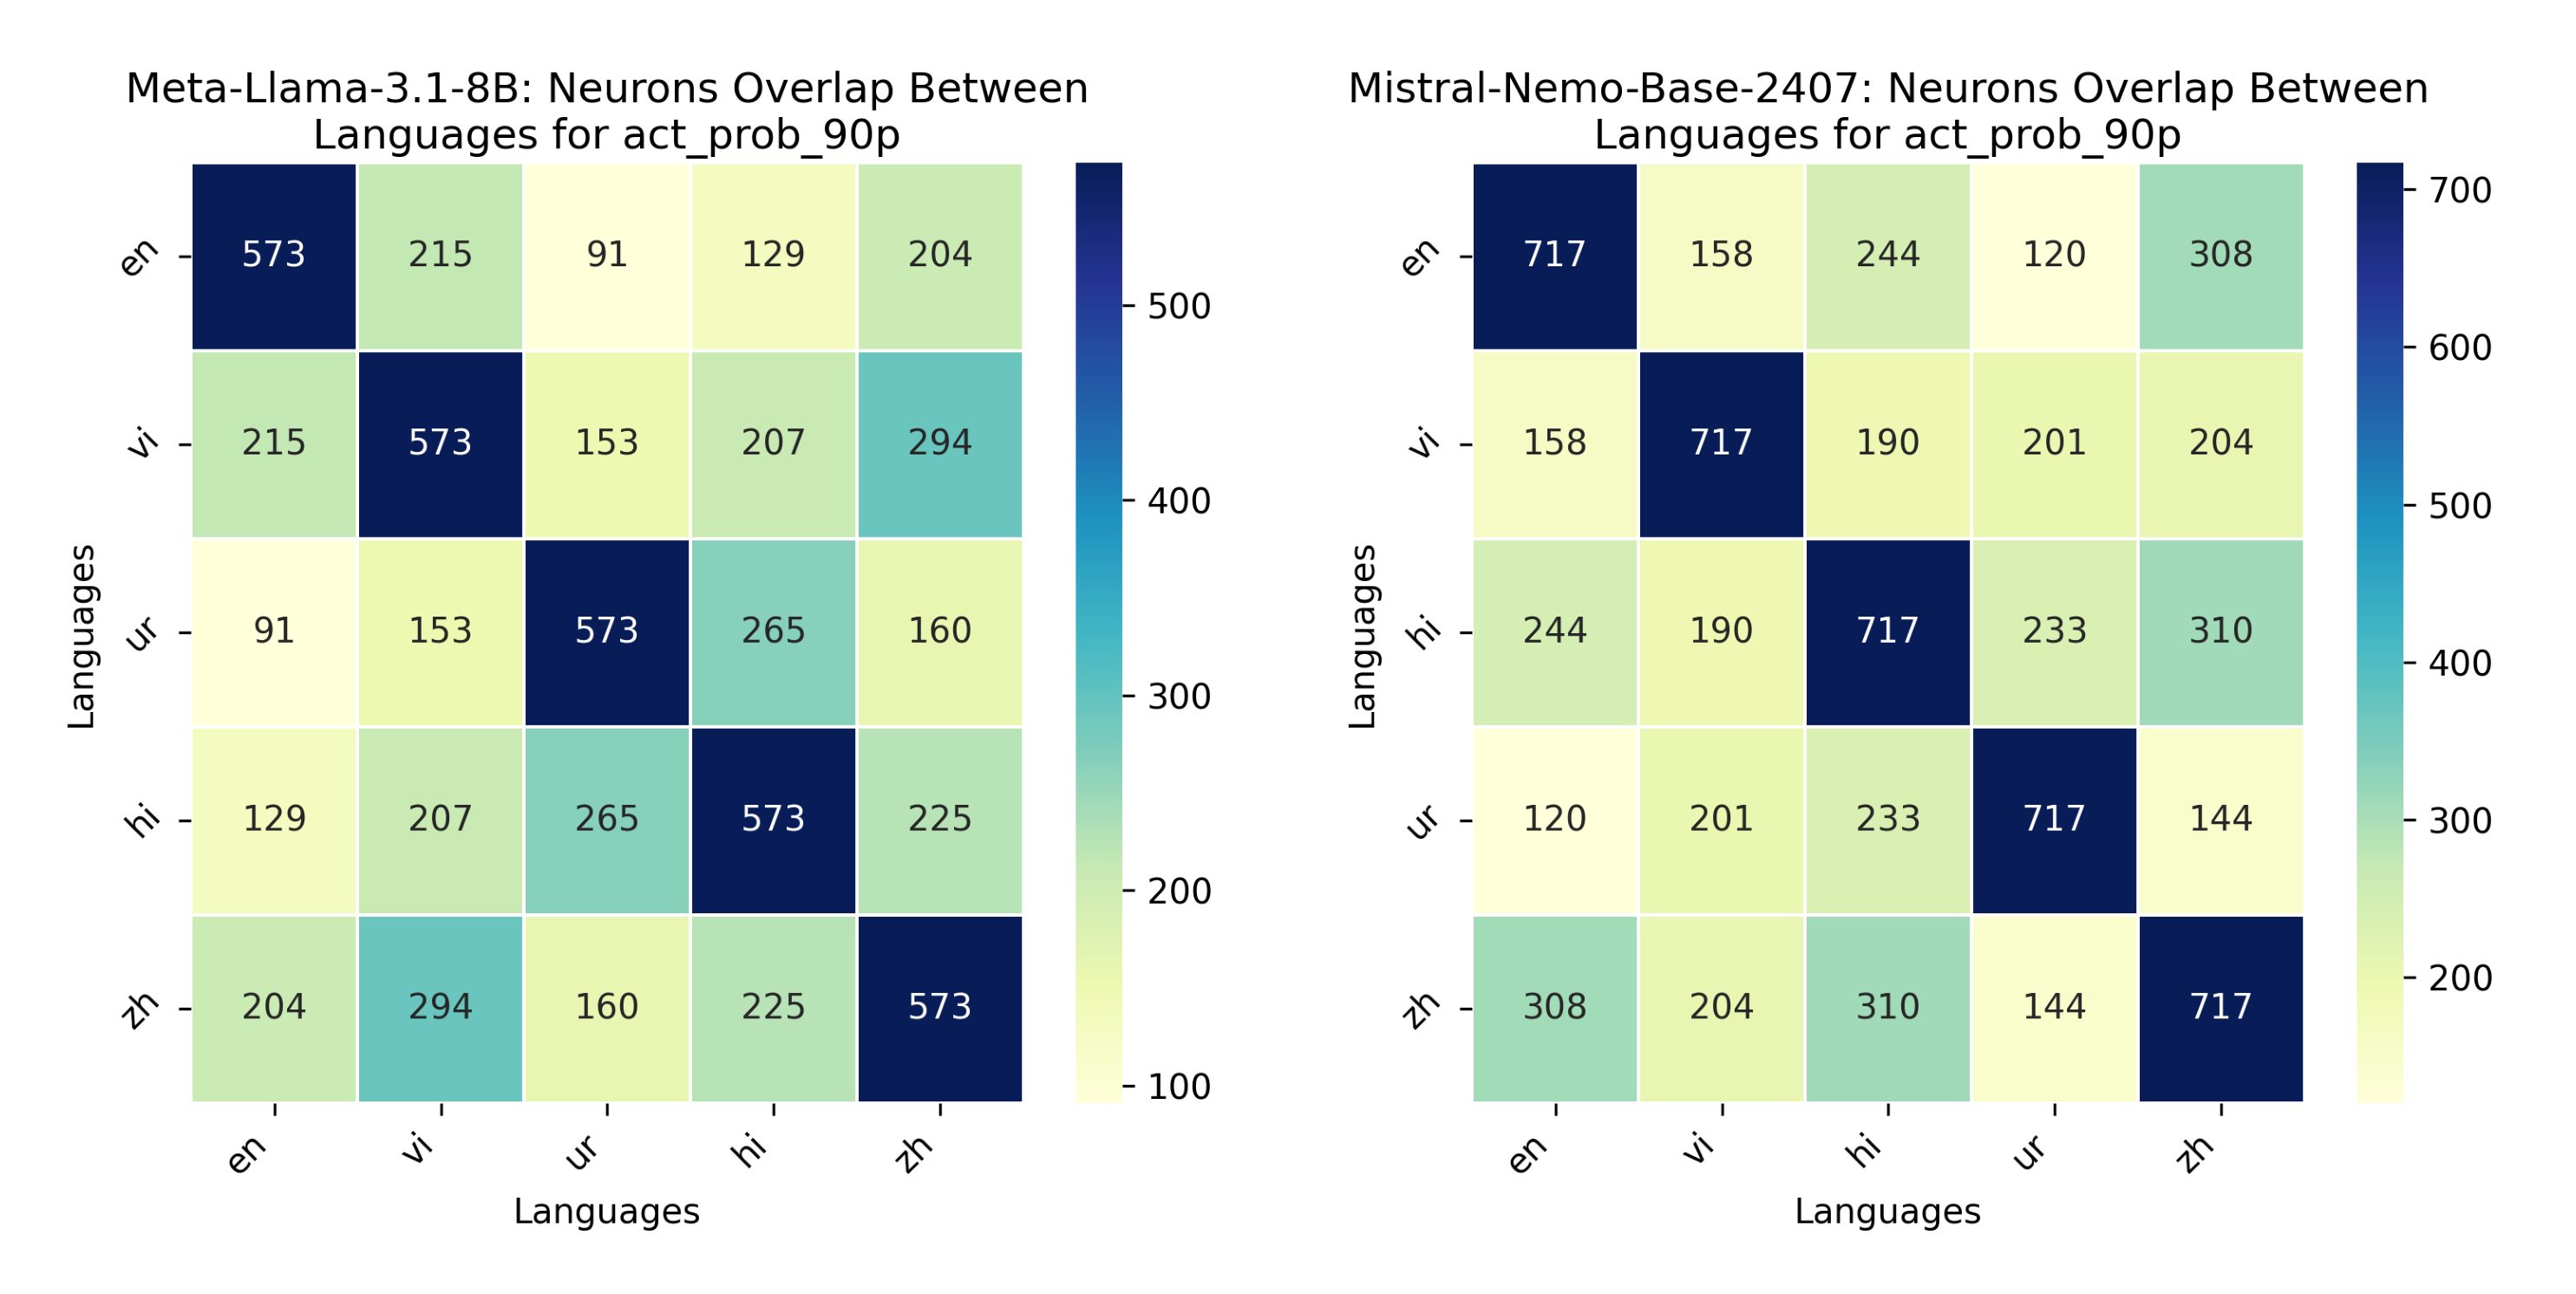
\includegraphics[width=0.8\linewidth]{Chapters/Chapter_3/figures/results/combined_act_lang_neurons_overlap.png}
	\caption{Overlap between the language-specific neuron sets under Act Prob 90p,
		for Llama~3.1 and Mistral Nemo. The diagonal is the size of each language's own
		set; the off-diagonal entries show that many neurons are shared across
		languages.}
	\label{fig:neurons-overlap-actprob}
\end{figure}

% FIGURE 3.5b (LAPE) -- include here.
% Suggested filename: fig_neuron_overlap_lape.png
% Content: pairwise neuron-set overlap heatmaps for LAPE, for Llama 3.1 and Mistral
% Nemo, on Set1 and Set6 (four panels).
\begin{figure}[ht]
	\centering
	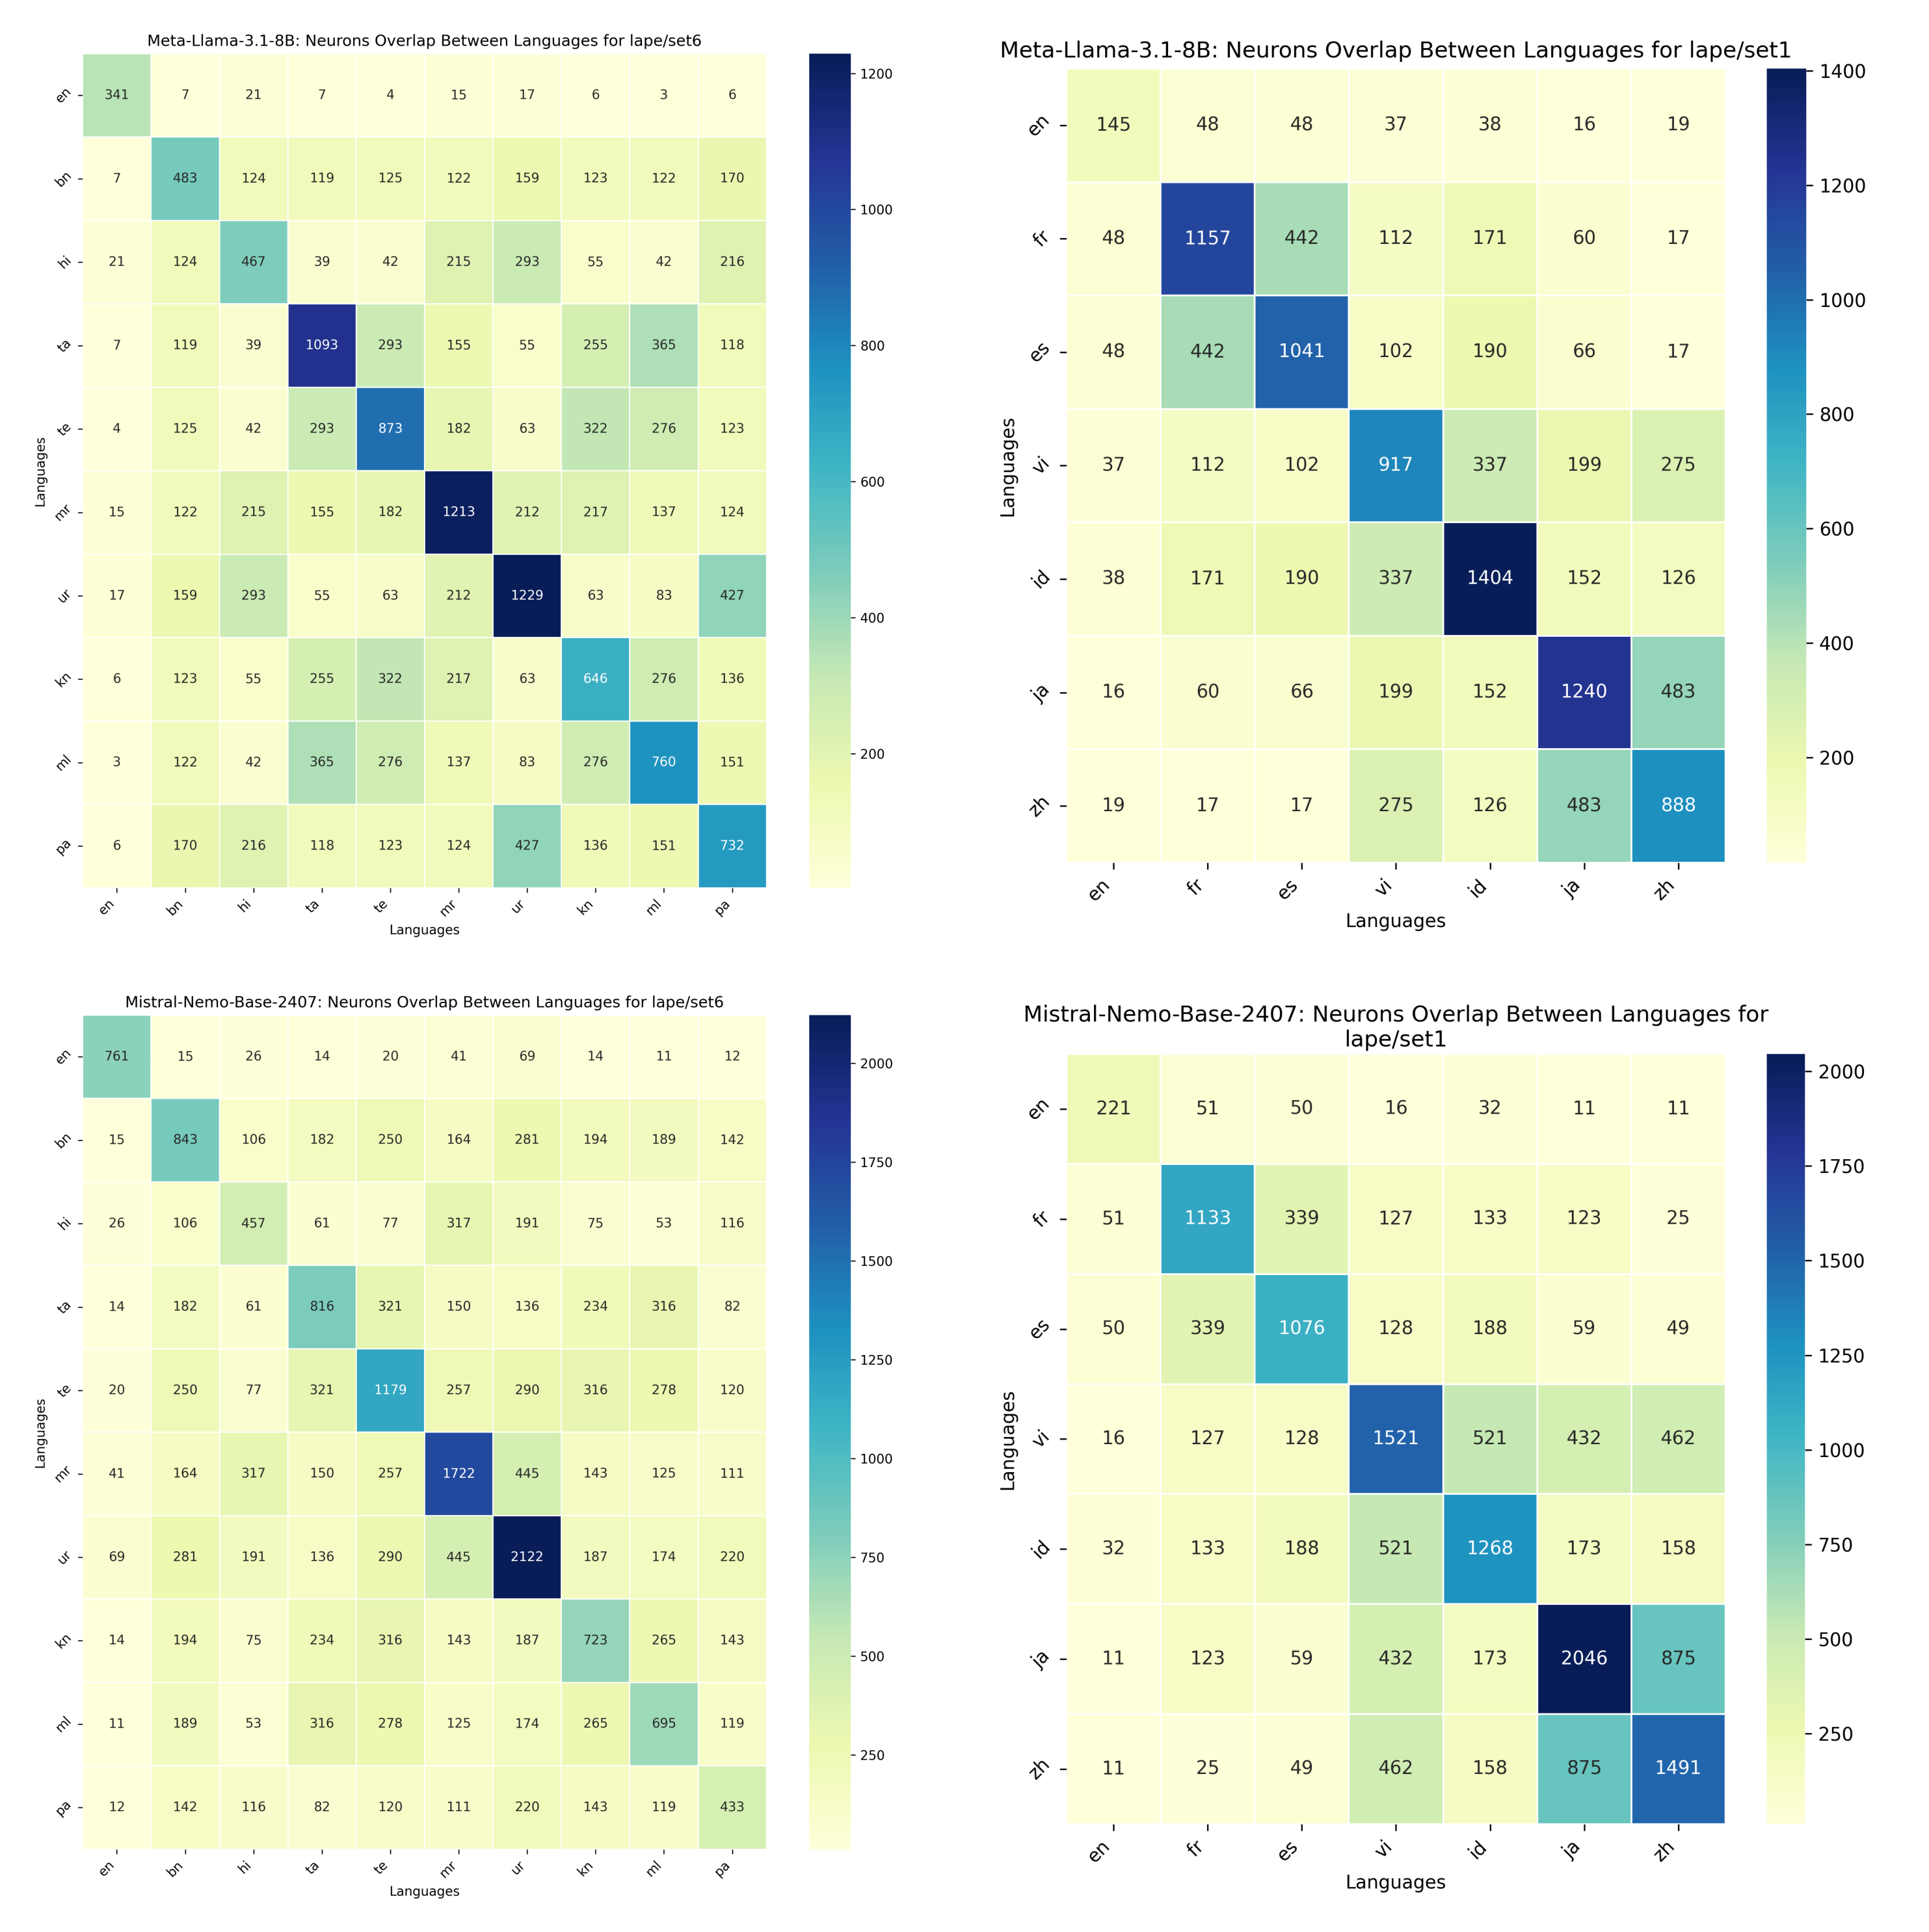
\includegraphics[width=0.8\linewidth]{Chapters/Chapter_3/figures/results/combined_lape_lang_neurons_overlap.png}
	\caption{Overlap between the language-specific neuron sets under LAPE, for
		Llama~3.1 and Mistral Nemo on Set1 and Set6. Related languages, such as Japanese
		and Chinese in Set1, share the most neurons.}
	\label{fig:neurons-overlap-lape}
\end{figure}

\subsection{Layer-Wise Distribution}
\label{subsec:neurons-layers}

We next look at where the identified neurons sit across the layers of the model.
Figure~\ref{fig:neurons-layers-lape} shows the distribution for LAPE, and
Figure~\ref{fig:neurons-layers-actprob} shows it for Act Prob 90p. The location of
the neurons depends on both the method and the model, and the two methods do not
agree.

Under LAPE, the neurons sit mostly in the upper part of the stack. For Llama~3.1
the counts are highest in the higher-middle layers, around layers 24 to 30, for
both Set1 and Set6. For Mistral Nemo the neurons concentrate in the topmost layers,
around layers 37 to 39, where the counts are much larger than anywhere else. The
bottom layers hold few neurons under LAPE, apart from a small number of isolated
cells.

Under Act Prob 90p the picture is different, and it also differs between the two
models. For Llama~3.1 the neurons are pushed towards the bottom of the stack: the
first layer holds a large number of English neurons, there is a strong band around
layers 3 and 4 across all languages, and the deeper layers stay sparse. For Mistral
Nemo the neurons sit in the middle of the stack, roughly layers 9 to 20, rather
than at either end, with the highest counts around layers 10 to 13 and layer 19.

So the two methods place language-specific neurons in different parts of the model,
and the layer pattern is not the same across the two models either. We point this
out because it matters for the discussion. As
Section~\ref{sec:neurons-results-transfer} shows, the two methods lead to the same
downstream conclusion even though they select neurons in different layers, which
means the result does not depend on where in the model the neurons are taken from.

% FIGURE 3.6a (LAPE) -- include here.
% Suggested filename: fig_neuron_layerwise_lape.png
% Content: layer-wise count of LAPE neurons per layer, for Llama 3.1 and Mistral
% Nemo, on Set1 and Set6 (four panels).
\begin{figure}[ht]
	\centering
	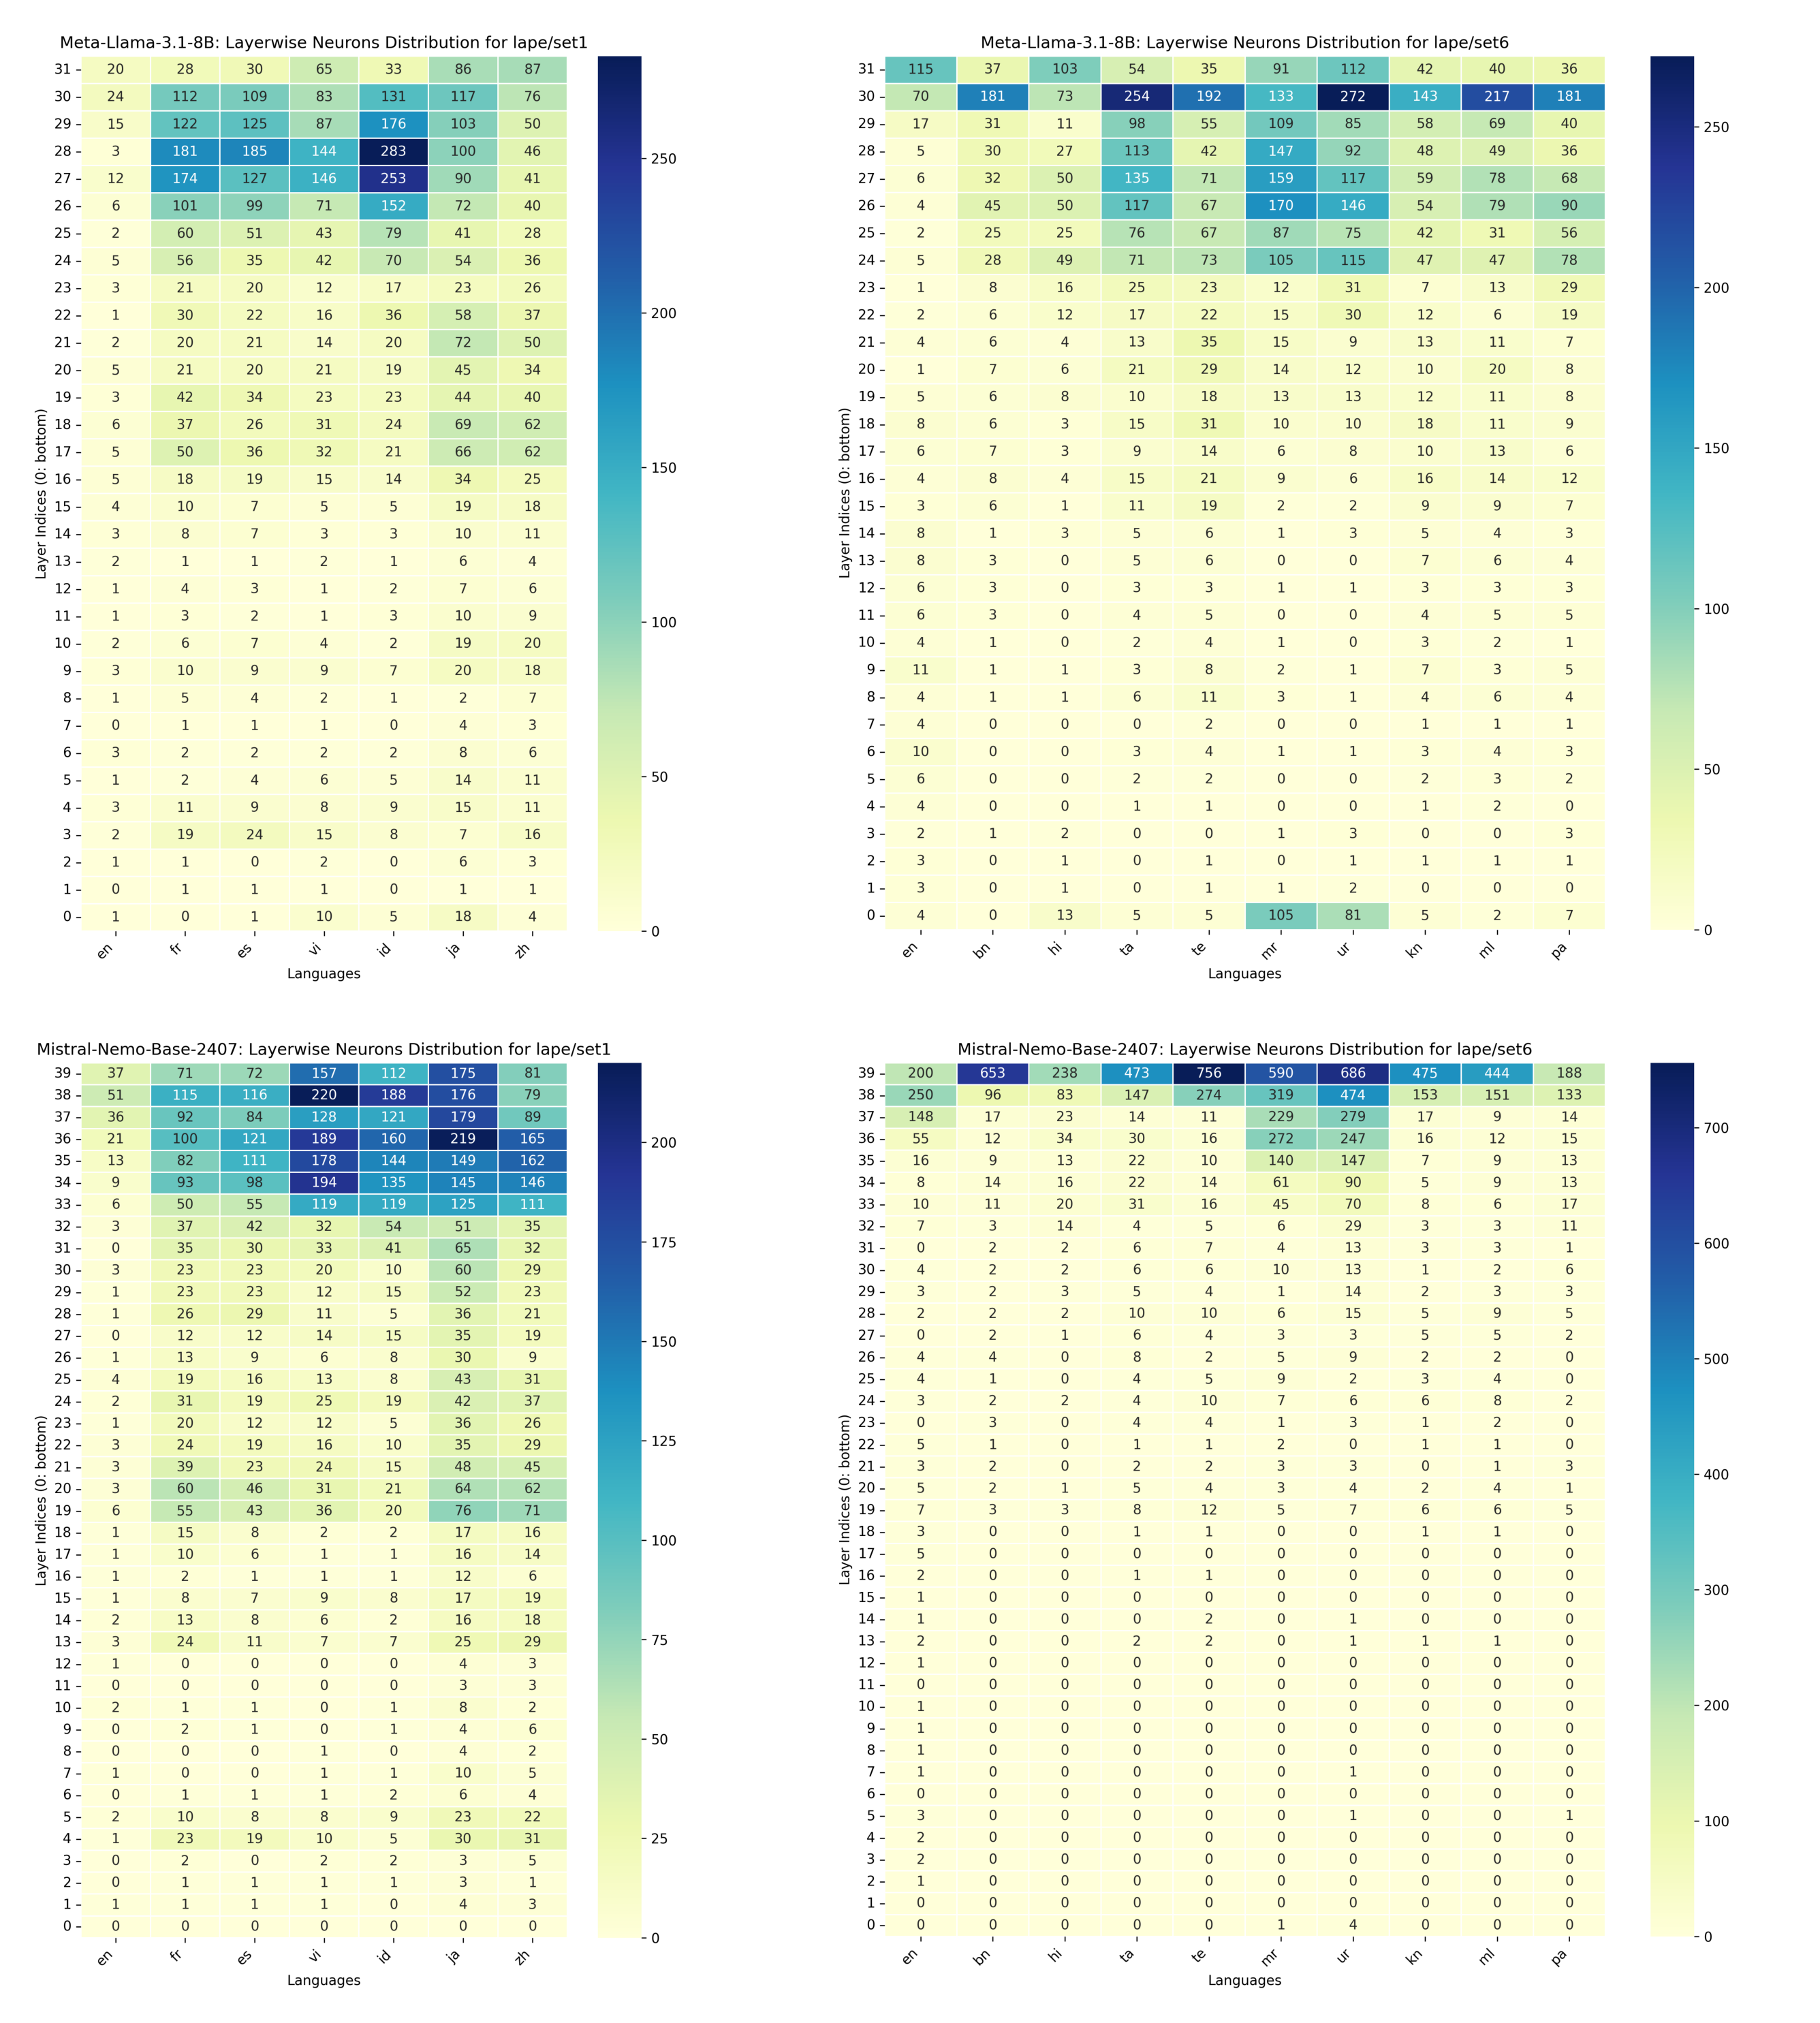
\includegraphics[width=0.8\linewidth]{Chapters/Chapter_3/figures/results/combined_lape_layerwise_lang_neurons_dist.png}
	\caption{Layer-wise distribution of language-specific neurons under LAPE, for
		Llama~3.1 and Mistral Nemo on Set1 and Set6. The neurons concentrate in the
		upper layers: the higher-middle layers for Llama~3.1 and the topmost layers for
		Mistral Nemo.}
	\label{fig:neurons-layers-lape}
\end{figure}

% FIGURE 3.6b (Act Prob 90p) -- include here.
% Suggested filename: fig_neuron_layerwise_actprob.png
% Content: layer-wise count of Act Prob 90p neurons per layer, for Llama 3.1 and
% Mistral Nemo.
\begin{figure}[ht]
	\centering
	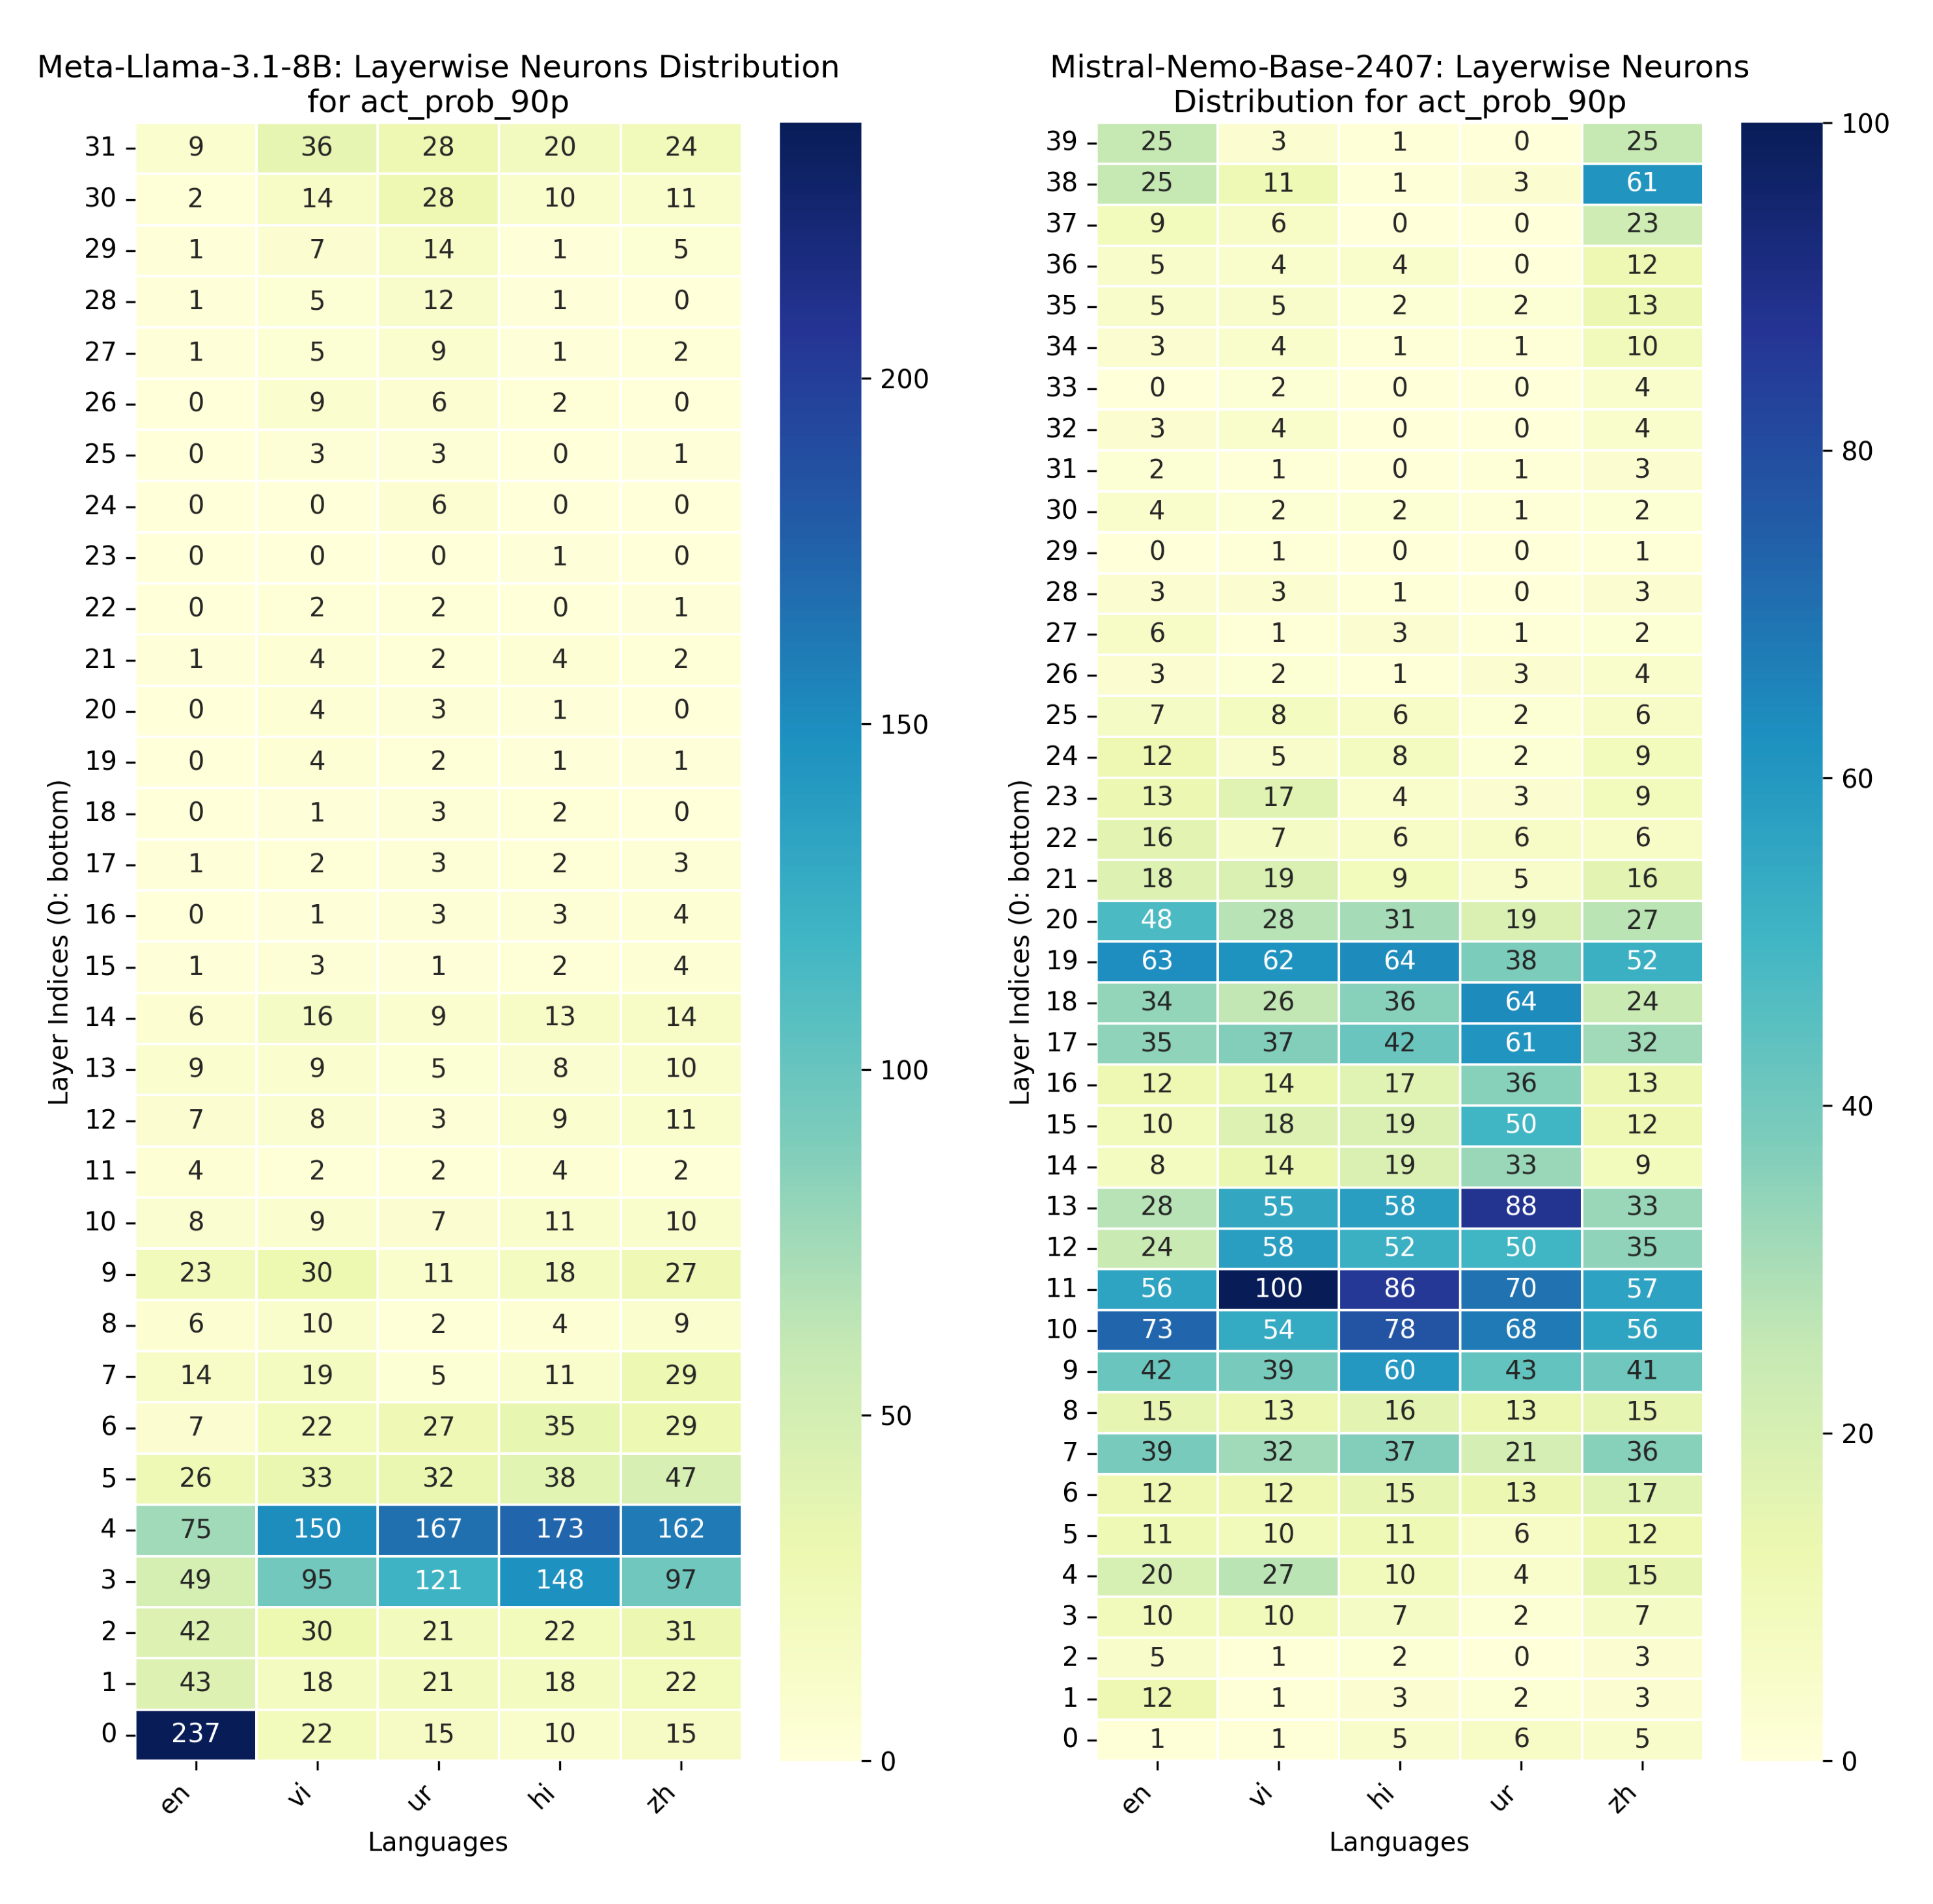
\includegraphics[width=0.8\linewidth]{Chapters/Chapter_3/figures/results/combined_act_layerwise_lang_neurons_dist.png}
	\caption{Layer-wise distribution of language-specific neurons under Act Prob
		90p, for Llama~3.1 and Mistral Nemo. The neurons sit at the bottom of the stack
		for Llama~3.1, with a large count in the first layer for English, and in the
		middle of the stack for Mistral Nemo.}
	\label{fig:neurons-layers-actprob}
\end{figure}

\subsection{Perplexity Change Under Intervention}
\label{subsec:neurons-ppxc-results}

We now check whether intervening on the neurons changes the model's handling of a
language, using the perplexity change of Equation~\ref{eq:neurons-ppxc}.
Figure~\ref{fig:neurons-ppxc} shows $\mathrm{PPXC}(i,j)$ as a heatmap, where row
$i$ is the language whose neurons are intervened on and column $j$ is the language
whose perplexity is measured. If the neurons were specific to their own language,
the diagonal ($i = j$) would be large and the off-diagonal entries small.

The heatmaps do not show this clean pattern. For most interventions the perplexity
change is small, including on the diagonal, which means that intervening on a
language's own neurons often does little to the model's perplexity on that
language. Where there are larger changes, they are not confined to the diagonal.
Setting activations to zero, in particular, does not produce the large diagonal
effect that would be expected if zero turned the neurons off. We take this up again
in the discussion, since it bears directly on the common practice of treating zero
as a way to deactivate a neuron.

% FIGURE 3.7 -- include here.
% Suggested filename: fig_ppxc_heatmap.pdf
% Content: PPXC heatmaps. Rows = language whose neurons are intervened on,
% columns = language whose perplexity is measured. Include the zero-intervention
% case (this is the publication's Figure 1) and, if available, the percentile
% cases, for LAPE and Act Prob 90p.
\begin{figure}[ht]
	\centering
	 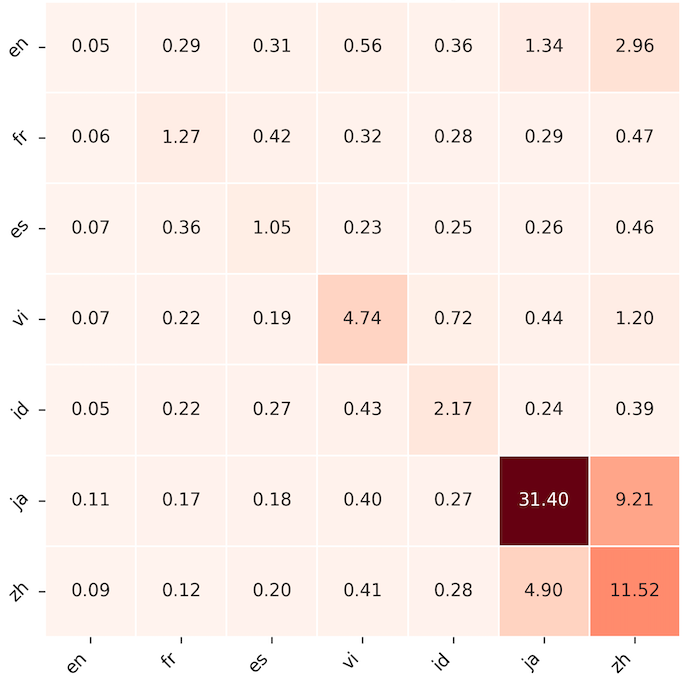
\includegraphics[width=0.6\linewidth]{Chapters/Chapter_3/figures/ppx.png}
	\caption{Perplexity change $\mathrm{PPXC}(i,j)$ under neuron intervention. Row
		$i$ is the language whose neurons are intervened on; column $j$ is the language
		whose perplexity is measured. Lower values mean the intervention has little
		effect. The changes are small for most interventions and are not concentrated
		on the diagonal.}
	\label{fig:neurons-ppxc}
\end{figure}

\section{Results: Cross-Lingual Transfer}
\label{sec:neurons-results-transfer}

We now turn to the main question, whether the interventions improve cross-lingual
task performance. We report results on XNLI and XQuAD, using English as the source
language and lower-resource languages as targets. For XNLI the target languages are
Vietnamese (vi), Hindi (hi), and Urdu (ur). For XQuAD they are Vietnamese (vi),
Hindi (hi), and Chinese (zh). In all settings the model is adapted using
English task data and evaluated on the target language without target-language task
data. The hyperparameters used for all fine-tuning runs are listed in
Table~\ref{tab:neurons-hyperparams}.

% TABLE 3.1 (hyperparameters) -- include here.
% Built from the published appendix (arXiv:2503.17456, App. B.2-B.3).
% Same settings apply to Llama 3.1 and Mistral Nemo; the only differences are
% per-task (XNLI vs XQuAD), so the table is organized by task.
\begin{table}[ht]
	\centering
	\begin{tabular}{lcc}
		\toprule
		\textbf{Setting} & \textbf{XNLI} & \textbf{XQuAD} \\
		\midrule
		\multicolumn{3}{l}{\textit{Models}} \\
		Backbones      & \multicolumn{2}{c}{Meta-Llama-3.1-8B, Mistral-Nemo-Base-2407} \\
		Quantization   & \multicolumn{2}{c}{4-bit (nf4), double quantization} \\
		Compute dtype  & \multicolumn{2}{c}{bfloat16} \\
		\midrule
		\multicolumn{3}{l}{\textit{LoRA}} \\
		Rank $r$              & 64    & 64    \\
		Scaling factor $\alpha$ & 128 & 128   \\
		\midrule
		\multicolumn{3}{l}{\textit{Optimization}} \\
		Optimizer          & AdamW & AdamW \\
		$\beta_1$, $\beta_2$ & 0.95, 0.999 & 0.95, 0.999 \\
		Learning rate      & $1\times10^{-6}$ & $5\times10^{-5}$ \\
		Weight decay       & 0.1   & 0.1   \\
		Gradient clipping  & 10.0  & 10.0  \\
		Warm-up            & 1\% of steps & 1\% of steps \\
		LR schedule        & linear decay & linear decay \\
		\midrule
		\multicolumn{3}{l}{\textit{Training}} \\
		Epochs             & 2     & 10    \\
		Batch size         & 8     & 4     \\
		Max context length & 256   & 512   \\
		Train split used   & 25\%  & 100\% \\
		Eval split used    & 100\% & 100\% \\
		\bottomrule
	\end{tabular}
	\caption{Hyperparameters for neuron-targeted fine-tuning on XNLI and XQuAD. The
		same settings are used for Llama~3.1 and Mistral Nemo; values differ only
		between the two tasks.}
	\label{tab:neurons-hyperparams}
	\end{table}

\subsection{Baseline}
\label{subsec:neurons-baseline}

Before applying any intervention, we record the no-intervention performance of each
model, which is the zero-shot cross-lingual transfer after adaptation on English
with no neuron edited. Table~\ref{tab:neurons-baseline} reports these numbers. They
are the reference for the rest of the section: an intervention is only useful if it
improves on this baseline. For XNLI we report accuracy on Vietnamese, Hindi, and
Urdu; for XQuAD we report exact match and, in parentheses, F1 on Vietnamese, Hindi,
and Chinese.

% TABLE 3.2 (baseline) -- include here.
% Built from the "No Int" column of the full XNLI and XQuAD result tables.
\begin{table}[ht!]
	\centering
	\renewcommand{\arraystretch}{1.2}
	\begin{tabular}{llcc}
		\toprule
		\textbf{Model} & \textbf{Eval Lang} & \textbf{XNLI (Acc \%)} & \textbf{XQuAD (EM (F1))} \\
		\midrule
		\multirow{3}{*}{Llama 3.1}   & vi      & 80.5 & 41 (73.5) \\
		& hi      & 75.0 & 38 (64.1) \\
		& ur / zh & 70.0 & 56 (77.5) \\
		\midrule
		\multirow{3}{*}{Mistral Nemo} & vi      & 80.5 & 39 (74.6) \\
		& hi      & 76.1 & 38 (66.9) \\
		& ur / zh & 66.8 & 47 (74.9) \\
		\bottomrule
	\end{tabular}
	\caption{No-intervention (zero-shot transfer) results for Llama~3.1 and Mistral Nemo. XNLI evaluates on vi/hi/ur (accuracy); XQuAD on vi/hi/zh (exact match with F1 in parentheses).}
	\label{tab:neurons-baseline}
\end{table}

\subsection{Test-Time Interventions}
\label{subsec:neurons-testtime-results}

Tables~\ref{tab:neurons-xnli-testtime} and~\ref{tab:neurons-xquad-testtime} report
the test-time intervention results on XNLI and XQuAD. In each table the baseline is
the No Int column, and the remaining columns replace the language-specific neuron
activations with the mean, with higher percentiles ($P75$, $P90$, $P95$), with
zero, and with lower percentiles ($P5$, $P10$, $P25$), for both identification
methods.

The main point is that no intervention improves the target languages as a group.
On XNLI, the best column for most rows is No Int, and where an intervention edges
above the baseline the gain is small, for example Llama~3.1 with LAPE on Hindi and
Urdu, where the mean intervention adds about two tenths of a point. These small
gains do not carry across languages or across the two models, so they read as noise
rather than a real effect.

The interventions do not only fail to help, they often hurt, and the size of the
damage depends on the model, the task, and the replacement value. For Llama~3.1 the
changes on XNLI stay within a few points. For Mistral Nemo they are much larger: the
lower-percentile and zero settings can pull accuracy down sharply, and with
Act~Prob~90p the $P5$ setting on Vietnamese drops from $80.5$ to the high thirties.
The lower percentiles are the most destructive overall, which fits the idea that
forcing these neurons to a low value disturbs computations the task depends on.

XQuAD shows the same pattern more strongly. The scores swing widely across
intervention columns, and several settings collapse the model: the mean
intervention takes Llama~3.1 with LAPE on Chinese from $56$ exact match to $10$,
and for Mistral~Nemo the higher-percentile and low-percentile settings drive
exact match to $0$ on some languages. As on XNLI, No Int is at or near the best
column for most rows, and no intervention lifts the three target languages together.

Setting the activations to zero is worth singling out, since zeroing is often used
as a way to switch a neuron off. The Int~0 column does not behave like removing a
needed component. On XNLI it stays close to the baseline in most rows, and on XQuAD
it is sometimes among the better intervention columns rather than the worst. This
matches the perplexity result in Section~\ref{subsec:neurons-ppxc-results}: zero is
just another value these activations can take, not an off state. The two
identification methods, LAPE and Act~Prob~90p, lead to the same overall picture, so
the outcome does not depend on how the neurons are chosen.

% TABLE 3.3 (XNLI test-time) -- paste the full XNLI intervention table here,
% converted to booktabs (toprule/midrule/bottomrule, no vertical bars).
% Label: tab:neurons-xnli-testtime
\begin{table}[t]
	\centering
	\renewcommand{\arraystretch}{1.2}
	\setlength{\tabcolsep}{5pt}
	\begin{small}
		\begin{tabular}{llcccccccc}
			\toprule
			\textbf{Model \& Method} & \textbf{Lang} & \textbf{No Int} & \textbf{Int} $\bm{\mu}$ & \textbf{P75} & \textbf{P90} & \textbf{P95} & \textbf{Int 0} & \textbf{P5} & \textbf{P10} \\
			\midrule
			\multirow{3}{*}{Llama 3.1 + LAPE}
			& vi & \textbf{80.5} & 79.5 & 79.1 & 79.0 & 78.9 & 79.8 & 73.6 & 77.7 \\
			& hi & 75.0 & \textbf{75.2} & 74.9 & 74.9 & 75.0 & 74.4 & 74.8 & 75.1 \\
			& ur & 70.0 & \textbf{70.4} & 70.2 & 69.3 & 69.0 & 68.5 & 68.6 & 68.7 \\
			\midrule
			\multirow{3}{*}{Llama 3.1 + Act Prob 90p}
			& vi & \textbf{80.5} & 78.2 & 78.9 & 79.3 & 79.5 & 79.0 & 76.5 & 77.4 \\
			& hi & \textbf{75.0} & 74.1 & 72.6 & 71.8 & 71.2 & 73.7 & 75.0 & 74.6 \\
			& ur & \textbf{70.0} & 69.7 & 69.7 & 69.3 & 68.7 & 69.6 & 69.4 & 69.5 \\
			\midrule
			\multirow{3}{*}{Mistral Nemo + LAPE}
			& vi & 80.5 & 80.4 & 80.5 & \textbf{80.6} & 80.5 & 79.2 & \textbf{80.6} & 80.5 \\
			& hi & \textbf{76.1} & 69.8 & 67.8 & 66.9 & 66.6 & 74.9 & 73.0 & 72.4 \\
			& ur & 66.8 & 66.5 & 67.2 & 67.0 & 66.8 & \textbf{66.9} & 65.8 & 65.4 \\
			\midrule
			\multirow{3}{*}{Mistral Nemo + Act Prob 90p}
			& vi & 80.5 & 67.4 & 79.0 & \textbf{81.1} & \textbf{81.1} & 79.8 & 37.4 & 40.7 \\
			& hi & \textbf{76.1} & 72.2 & 73.7 & 74.5 & 74.4 & 74.5 & 62.4 & 66.3 \\
			& ur & \textbf{66.8} & 65.9 & 64.0 & 61.3 & 59.7 & 66.4 & 54.6 & 61.6 \\
			\bottomrule
		\end{tabular}
	\end{small}
	\caption{XNLI test-time intervention accuracy. No Int is the baseline; the other
		columns set the language-specific neuron activations to the mean, to higher
		percentiles, to zero, and to lower percentiles, for LAPE and Act Prob 90p. The
		best value in each row is in bold. No intervention improves the three target
		languages as a group, and the lower-percentile and zero settings often degrade
		accuracy, most clearly for Mistral Nemo.}
	\label{tab:neurons-xnli-testtime}
\end{table}

% TABLE 3.4 (XQuAD test-time) -- paste the full XQuAD intervention table here,
% converted to booktabs. Each cell is EM (F1). Label: tab:neurons-xquad-testtime
\begin{table}[t]
	\centering
	\renewcommand{\arraystretch}{1.3}
	\setlength{\tabcolsep}{3.5pt}
	\begin{scriptsize}
		\begin{tabular}{llcccccccc}
			\toprule
			\textbf{Model \& Method} & \textbf{Lang} & \textbf{No Int} & \textbf{Int} $\bm{\mu}$ & \textbf{P75} & \textbf{P90} & \textbf{P95} & \textbf{Int 0} & \textbf{P5} & \textbf{P10} \\
			\midrule
			\multirow{3}{*}{Llama 3.1 + LAPE}
			& vi & 41 (73.5) & 40 (72.9) & 36 (76.7) & 31 (69.5) & 28 (66.8) & 32 (69.2) & 4 (35.8) & 10 (43.2) \\
			& hi & 38 (64.1) & 40 (65.5) & 38 (66.4) & 36 (65.4) & 36 (66.3) & 23 (49.9) & 38 (62.8) & 37 (62.8) \\
			& zh & 56 (77.5) & 10 (62.8) & 3 (58.1) & 3 (56.1) & 4 (52.9) & 33 (63.2) & 20 (49.1) & 33 (63.2) \\
			\midrule
			\multirow{3}{*}{Llama 3.1 + Act Prob 90p}
			& vi & 41 (73.6) & 39 (73.0) & 26 (65.8) & 23 (64.9) & 24 (64.8) & 42 (73.8) & 33 (67.8) & 36 (70.3) \\
			& hi & 38 (64.1) & 34 (60.7) & 35 (62.3) & 36 (62.8) & 32 (61.9) & 38 (62.9) & 23 (54.9) & 31 (58.6) \\
			& zh & 56 (77.5) & 61 (80.7) & 59 (79.5) & 56 (78.8) & 56 (78.4) & 55 (78.5) & 40 (61.7) & 50 (73.6) \\
			\midrule
			\multirow{3}{*}{Mistral Nemo + LAPE}
			& vi & 39 (74.6) & 42 (76.8) & 40 (76.4) & 40 (75.0) & 39 (73.6) & 13 (45.0) & 10 (40.4) & 11 (41.2) \\
			& hi & 38 (66.9) & 35 (65.9) & 38 (67.1) & 37 (66.6) & 34 (66.5) & 22 (51.7) & 36 (65.8) & 36 (66.1) \\
			& zh & 47 (74.9) & 24 (74.0) & 4 (65.6) & 0 (61.6) & 0 (59.3) & 14 (53.3) & 1 (33.6) & 24 (68.9) \\
			\midrule
			\multirow{3}{*}{Mistral Nemo + Act Prob 90p}
			& vi & 39 (74.6) & 11 (43.3) & 26 (62.8) & 29 (63.9) & 15 (48.5) & 39 (74.5) & 0 (3.8) & 0 (6.5) \\
			& hi & 38 (66.9) & 26 (54.4) & 34 (65.1) & 37 (68.9) & 37 (68.7) & 33 (63.8) & 0 (6.0) & 0 (11.9) \\
			& zh & 47 (74.9) & 46 (77.4) & 26 (69.9) & 20 (59.8) & 15 (54.9) & 48 (76.2) & 0 (8.5) & 0 (17.0) \\
			\bottomrule
		\end{tabular}
	\end{scriptsize}
	\caption{XQuAD test-time intervention results, reported as exact match with F1
		in parentheses, for the same intervention columns as
		Table~\ref{tab:neurons-xnli-testtime}. The pattern matches XNLI but the swings
		are larger: several settings collapse the score, such as Llama~3.1 with LAPE on
		Chinese under the mean intervention and Mistral~Nemo under the higher- and
		lower-percentile settings. No intervention lifts the three target languages
		together.}
	\label{tab:neurons-xquad-testtime}
\end{table}

\subsection{Neuron Fine-Tuning}
\label{subsec:neurons-ft}

The test-time interventions in
Section~\ref{subsec:neurons-testtime-results} fixed the neuron activations to a
chosen value. Here we instead fine-tune the identified neurons, so the model can
adjust them through training rather than having them set by hand.
Table~\ref{tab:neurons-ft} reports this for Llama~3.1 on XNLI, for both
identification methods and under the three fine-tuning-language (FTL) settings from
Section~\ref{subsec:neurons-config}: fine-tuning the source-language (English)
neurons, the target-language neurons, or both. The task training data is always
English. For each fine-tuned model we also apply the test-time interventions, so
each row shows the no-intervention score next to the mean, $P90$, zero, and $P10$
settings.

Two things stand out. First, for Vietnamese and Hindi the no-intervention column is
the best or close to the best in every row, for both LAPE and Act~Prob~90p.
Fine-tuning the neurons and then intervening on them does not beat simply
fine-tuning and leaving the neurons alone. Second, the choice of which language's
neurons are made trainable barely changes the result. Within a target language the
three FTL settings give almost the same scores, for example Vietnamese stays near
$80.1$ under LAPE whether we fine-tune the English neurons, the Vietnamese neurons,
or both. If the language-specific neurons carried information that transfers to the
target language, we would expect fine-tuning the target-language neurons to help
more than fine-tuning the English ones, and we do not see that.

The one place any column edges above the baseline is Urdu, where the mean
intervention reaches about $70.4$ to $70.6$ against a baseline near $70.0$. This is
a fraction of a point, it appears only for one language, and it does not hold for
Vietnamese or Hindi, so it is not evidence that the approach works. The pattern is
the same under Act~Prob~90p as under LAPE. Since Act~Prob~90p does not depend on the
choice of language set, while LAPE does, the agreement between the two also rules
out the language-set normalization in LAPE as the reason for the negative result.
Overall the fine-tuning experiment points the same way as the test-time one: acting
on the identified neurons does not improve cross-lingual transfer.

% TABLE 3.5 (neuron fine-tuning, XNLI, Llama 3.1) -- booktabs style, no vertical
% bars. LAPE and Act Prob 90p in one table, split by section rows.
% Label: tab:neurons-ft
\begin{table}[ht!]
	\centering
	\renewcommand{\arraystretch}{1.15}
	\setlength{\tabcolsep}{6pt}
	\footnotesize
	\begin{tabular}{llccccc}
		\toprule
		\textbf{FTL} & \textbf{EL} & \textbf{No Int} & \textbf{Int} $\bm{\mu}$ & \textbf{Int P90} & \textbf{Int 0} & \textbf{Int P10} \\
		\midrule
		\multicolumn{7}{c}{\textit{Llama 3.1 with LAPE}} \\
		\midrule
		en     & vi & \textbf{80.2} & 79.6 & 78.5 & 79.2 & 78.0 \\
		vi     & vi & \textbf{80.1} & 79.5 & 78.6 & 79.2 & 78.0 \\
		en+vi  & vi & \textbf{80.1} & 79.4 & 78.5 & 79.1 & 78.0 \\
		\midrule
		en     & hi & \textbf{74.9} & 74.6 & 74.6 & 74.1 & 74.6 \\
		hi     & hi & \textbf{74.9} & 74.6 & 74.5 & 74.3 & 74.6 \\
		en+hi  & hi & \textbf{74.9} & 74.5 & 74.5 & 74.3 & 74.7 \\
		\midrule
		en     & ur & 69.8 & \textbf{70.4} & 69.6 & 70.2 & 69.0 \\
		ur     & ur & \textbf{69.8} & 70.5 & 69.5 & 70.4 & 69.1 \\
		en+ur  & ur & 70.0 & \textbf{70.6} & 69.5 & 70.3 & 68.9 \\
		\midrule
		\multicolumn{7}{c}{\textit{Llama 3.1 with Act Prob 90p}} \\
		\midrule
		en     & vi & \textbf{80.3} & 78.0 & 79.1 & 78.5 & 77.5 \\
		vi     & vi & \textbf{80.1} & 78.0 & 79.0 & 78.7 & 77.4 \\
		en+vi  & vi & \textbf{80.1} & 78.0 & 78.9 & 78.8 & 77.4 \\
		\midrule
		en     & hi & \textbf{74.9} & 73.9 & 72.1 & 73.3 & 74.5 \\
		hi     & hi & \textbf{74.9} & 73.8 & 72.1 & 73.9 & 74.6 \\
		en+hi  & hi & \textbf{74.9} & 73.7 & 72.1 & 73.8 & 74.6 \\
		\midrule
		en     & ur & 69.9 & \textbf{70.1} & 69.4 & 70.0 & 69.5 \\
		ur     & ur & 69.9 & 70.0 & 69.4 & \textbf{70.1} & 69.5 \\
		en+ur  & ur & 69.8 & 69.9 & 69.3 & \textbf{70.1} & 69.6 \\
		\bottomrule
	\end{tabular}
	\caption{Neuron fine-tuning results for Llama~3.1 on XNLI, for LAPE and
		Act~Prob~90p. FTL is the fine-tuning language (English, the target, or both);
		EL is the evaluation language; task training data is always English. Each
		fine-tuned model is also evaluated under the test-time interventions (mean,
		$P90$, zero, $P10$). The best value in each row is in bold. No~Int is the best
		column in nearly every row, and the FTL setting has little effect, so
		fine-tuning the identified neurons does not improve cross-lingual transfer.}
	\label{tab:neurons-ft}
\end{table}

\subsection{Random-Neuron Control}
\label{subsec:neurons-random}

The interventions so far act on neurons that a method marked as language-specific.
A natural question is whether these neurons matter more than any other neurons. To
check this, we run a control in which we fine-tune randomly chosen neurons instead
of the identified ones, keeping the number of fine-tuned neurons the same (ten per
layer). Everything else, including the English task training and the evaluation
setup, is unchanged. Table~\ref{tab:neurons-random} reports the zero-shot
(No~Int) accuracy after this random-neuron fine-tuning.

The scores are close to those from fine-tuning the language-specific neurons in
Table~\ref{tab:neurons-ft}. For Llama~3.1, random-neuron fine-tuning gives $80.1$
on Vietnamese, $74.8$ on Hindi, and $69.8$ on Urdu, which are within a fraction of
a point of the corresponding language-specific runs. If the identified neurons
carried information that ordinary neurons did not, fine-tuning them should beat
fine-tuning random ones, and we do not see that gap. This is what we would expect
if the selected neurons are not doing anything special for the task that other
neurons cannot also do, and it fits the overlap and polysemanticity results
discussed earlier. The control therefore supports the same conclusion as the rest
of the section: the negative result is not because we picked the wrong neurons, but
because acting on a small set of neurons, identified or random, does not change
cross-lingual transfer.

% TABLE 3.6 (random-neuron control) -- booktabs style, no vertical bars.
% Label: tab:neurons-random
\begin{table}[ht!]
	\centering
	\renewcommand{\arraystretch}{1.3}
	\setlength{\tabcolsep}{8pt}
	\footnotesize
	\begin{tabular}{llcc}
		\toprule
		\textbf{Model} & \textbf{FTL} & \textbf{EL} & \textbf{No Int} \\
		\midrule
		\multirow{3}{*}{Llama 3.1}    & rand & vi & 80.1 \\
		& rand & hi & 74.8 \\
		& rand & ur & 69.8 \\
		\midrule
		\multirow{3}{*}{Mistral Nemo} & rand & vi & 80.4 \\
		& rand & hi & 75.6 \\
		& rand & ur & 65.5 \\
		\bottomrule
	\end{tabular}
	\caption{Random-neuron control. Zero-shot (No~Int) XNLI accuracy after
		fine-tuning ten randomly selected neurons per layer, instead of the
		language-specific neurons, for Llama~3.1 and Mistral~Nemo. The scores are close
		to the language-specific fine-tuning results in
		Table~\ref{tab:neurons-ft}, so the identified neurons are not doing something
		other neurons cannot.}
	\label{tab:neurons-random}
\end{table}

\section{Discussion}
\label{sec:neurons-discussion}

The results are consistent in their conclusion across tasks, models, and
identification methods: interventions on language-specific neurons do not give a
reliable improvement in cross-lingual task performance. This section discusses why.

\subsection{Polysemantic Neurons and Entangled Function}
\label{subsec:neurons-polysemantic}

The neuron analysis points to one explanation. The identified neurons are shared
across languages (Section~\ref{subsec:neurons-overlap}), and the random-neuron
control (Section~\ref{subsec:neurons-random}) gives almost the same scores as
fine-tuning the identified neurons, so the selected neurons are not doing anything
that other neurons cannot. This fits the idea that a single neuron takes part in
more than one function, often called polysemanticity
\citep{elhage2022superposition}. If a neuron contributes to several computations at
once, including ones the task depends on, then fixing its activation or restricting
fine-tuning to it disturbs those other computations as well. The intervention is
not surgical, even though the neuron was selected as language-specific.

\subsection{Zero Is Not Deactivation}
\label{subsec:neurons-zero}

A common way to test a neuron's role is to set its activation to zero and see what
breaks. Our results show this is not a safe assumption here. Setting the activations
to zero does not produce a large perplexity change
(Section~\ref{subsec:neurons-ppxc-results}), and the Int~0 column does not collapse
task performance the way removing a needed component would
(Section~\ref{subsec:neurons-testtime-results}); on XQuAD it is sometimes among the
better intervention columns rather than the worst. For these activations, zero is
just another value the neuron can take, not an off state. Conclusions that rely on
zeroing a neuron to measure its importance should be treated with care.

\subsection{Neurons Are Not Independent Across Languages}
\label{subsec:neurons-independence}

The overlap between the language sets
(Section~\ref{subsec:neurons-overlap}) and the off-diagonal perplexity changes
(Section~\ref{subsec:neurons-ppxc-results}) both show that the neurons for one
language are tied to those of others. This matters for the original goal. The
appeal of language-specific neurons was that one could improve a target language by
acting on its own neurons. If those neurons are shared with other languages, there
is no clean handle to act on, and an edit aimed at one language reaches the others
as well.

\subsection{The Result Does Not Depend on How Neurons Are Selected}
\label{subsec:neurons-consistency}

LAPE and Act~Prob~90p score and select neurons differently. They also place the
selected neurons in different parts of the model: as the layer-wise and overlap
results show (Section~\ref{subsec:neurons-layers},
Section~\ref{subsec:neurons-overlap}), LAPE concentrates neurons in the upper
layers while Act~Prob~90p places them at the bottom for Llama~3.1 and in the middle
for Mistral~Nemo, and the two methods select largely different sets. Despite this,
they lead to the same downstream conclusion in every experiment. The fact that two
methods which disagree on which neurons are language-specific, and where they sit,
still produce the same outcome makes it unlikely that the negative result is an
artifact of one selection rule or of the language-set normalization that LAPE
depends on. It points instead to a property of how language is represented in these
models, rather than of how we pick the neurons.

\section{Limitations}
\label{sec:neurons-limitations}

This study has several limitations. It looks only at neurons in the MLP layers and
does not consider the attention mechanism, which may also carry language-specific
behaviour. The experiments use a small number of languages and two datasets, so the
findings may not extend to all languages or tasks. The test-time interventions use
statistics computed from Wikipedia text, which may not match how neurons behave on
task inputs. The fine-tuning experiments are run on Llama~3.1, so the fine-tuning
conclusions are not separately confirmed on Mistral~Nemo. Finally, the study uses
LoRA-based fine-tuning and does not explore other fine-tuning methods that might
interact with the neurons differently. These points mark where the conclusion is
and is not expected to hold.

\chapter{Cross-Lingual Mechanisms during GRPO Training}
\label{ch:grpo-crosslingual}

\section{Introduction}
\label{sec:grpo-intro}

\subsection{Motivation}
\label{subsec:grpo-motivation}

Chapter~\ref{ch:neurons} asked where language sits inside a fixed model and found
that editing a localized set of neurons does not change what the model does on a
task. This chapter asks a different question. Instead of probing a fixed model, we
watch how a training procedure changes a model's cross-lingual behaviour over time.
The procedure is Group Relative Policy Optimization (GRPO), a reinforcement learning
method used to fine-tune models for reasoning, and the behaviour we track is how the
model handles the same math problem posed in different languages.

There is a common claim about how multilingual models process non-English input.
The claim, which we call the Wendler three-phase hypothesis
\citep{wendler2024llamas}, is that the model maps the input into an English-aligned
space in the early layers, works in that space through the middle layers, and maps
back to the input language only in the last few layers. If this is right, then
reading out the language of the model's intermediate predictions should show English
through the body of the stack and the target language only at the end.

This matters once reinforcement learning enters. GRPO rewards the model based on
whether the final answer is correct, judged by a verifier that reads only the
answer, not the language of the reasoning. If the model could raise its reward by
leaning more on an English-aligned middle of the stack, then training might push it
in that direction and widen the gap for low-resource languages. Whether GRPO
actually changes this internal behaviour, and how its effect varies across
languages, is what we study.

\subsection{Problem Statement}
\label{subsec:grpo-problem}

We study how GRPO fine-tuning changes the cross-lingual behaviour of a multilingual
math reasoner. This breaks into the following parts.

\begin{enumerate}
	\item \textbf{Does GRPO change accuracy, and does it do so evenly across
		languages?} We track per-language accuracy across training to see how much, and
	for which languages, GRPO moves the task performance.
	
	\item \textbf{Does the model predict in English in the middle layers, and does
		GRPO change this?} The three-phase hypothesis describes an English-leaning
	middle of the stack. We check whether this is present, and whether training
	makes it stronger or weaker, using the language of the model's intermediate
	predictions.
	
	\item \textbf{Which languages does GRPO struggle with, and what is happening
		inside the model for them?} For a language that GRPO does not improve, we ask
	whether its representations are left alone or are changed without any matching
	accuracy gain, and what sets such a language apart from the rest.
\end{enumerate}

\subsection{Contributions}
\label{subsec:grpo-contributions}

This chapter reports the following.

\begin{itemize}
	\item We fine-tune Qwen2.5-7B-Instruct on the seven-language MGSM benchmark with
	GRPO and a low-rank adapter, save checkpoints across 620 gradient steps, and
	study the model along five lines: end-task accuracy, the per-layer language of
	logit-lens predictions, a three-phase categorical analysis of those predictions,
	the gap between English and the target language, and the geometry of the
	representations measured with Centred Kernel Alignment.
	
	\item We find that GRPO moves accuracy very little for any of these languages.
	Six of the seven stay in a band between about $0.72$ and $0.94$ and change by at
	most a few points over training, and Telugu stays far below the rest, at about
	$0.38$ to $0.40$, throughout.
	
	\item We find that GRPO does not cause cross-lingual collapse. The model already
	reads out as English through the early and middle layers and surfaces the target
	language only in the last few layers, and this is present from the start and
	does not change over 620 GRPO steps. Training neither builds up nor removes the
	English-leaning middle of the stack.
	
	\item We show that Telugu, the language that sits far below the rest, is also the
	one whose representations GRPO changes the most, while its accuracy does not
	move. We connect this to tokeniser coverage: Telugu has very few dedicated tokens
	in the Qwen2.5 vocabulary, and we argue that the limiting factor for GRPO here is
	the granularity of the reward signal, not language identity or a change in the
	model's internal routing.
\end{itemize}

\section{Background}
\label{sec:grpo-background}

\subsection{The Three-Phase Hypothesis}
\label{subsec:grpo-wendler}

Work on how multilingual transformers process input has suggested a three-phase
picture \citep{wendler2024llamas}. In the early layers the model maps the input
tokens into its internal representation. In the middle layers it works in a space
closer to English than to the input language, so a tool that reads out the model's
intermediate state would see English-like predictions even when the input is in
another language. In the last layers the model maps back to the input language to
produce the output. We call this the early-target, mid-English, late-target
structure.

The hypothesis matters here for two reasons. First, it makes a static prediction:
reading out the language of the model's intermediate predictions should show English
through the body of the stack and the target language only near the end. Second, and
more important for us, it raises a training question. Since the GRPO reward depends
only on the final answer and not on the language of the reasoning, training could
push the model to lean even more on an English-aligned middle. We test the static
prediction, and by tracking it across checkpoints, we test whether GRPO changes it.

\subsection{Group Relative Policy Optimization}
\label{subsec:grpo-objective}

GRPO \citep{shao2024deepseekmath} is an online policy-gradient method. For a prompt,
the policy generates a group of responses, each scored by a reward function. Instead
of using a separate value model to compute a baseline, GRPO standardizes the rewards
within the group and uses that as the advantage.

Let $\pi_\theta$ be the policy, $\pi_{\theta_{\text{old}}}$ the policy at the start
of the current rollout, and $\pi_{\text{ref}}$ a frozen reference policy. For a
prompt $i$, the policy generates $G$ responses $\{y_{i,j}\}_{j=1}^G$, and each
receives a scalar reward $R_i^j$. The group-relative advantage standardizes the
rewards within the group:
\begin{equation}
	\mu^i = \frac{1}{G} \sum_{j=1}^{G} R_i^j, \qquad
	\sigma^i = \sqrt{\frac{1}{G} \sum_{j=1}^{G} (R_i^j - \mu^i)^2}, \qquad
	A_i^j = \frac{R_i^j - \mu^i}{\sigma^i}.
	\label{eq:grpo-advantage}
\end{equation}
The advantage is the same for every token in a response. The per-response objective
uses a clipped policy ratio with a KL penalty against the reference policy, in the
usual GRPO form, and the per-batch loss averages this over the group and the batch:
\begin{equation}
	\mathcal{L}_{\text{GRPO}}(\theta) = -\frac{1}{B} \sum_{i=1}^{B} \frac{1}{G} \sum_{j=1}^{G} \mathcal{L}_{i,j}^{\text{resp}},
	\label{eq:grpo-loss}
\end{equation}
where $B$ is the batch size. We use a clipping range $\epsilon = 0.2$ and a KL
coefficient $\beta = 0.04$. The reward is binary, based on whether an external judge
accepts the final answer, and is described in Section~\ref{subsec:grpo-reward}.

\subsection{Tools for Looking Inside the Model}
\label{subsec:grpo-tools}

Two tools from Chapter~\ref{ch:related-work} are used throughout. The logit lens
\citep{nostalgebraist2020logitlens} reads out what the model would predict at an
intermediate layer by applying the model's final normalization and output head to
that layer's residual-stream activation, giving a distribution over the vocabulary
at each layer. We use it to ask, at each layer, which language the model's predicted
token belongs to. Centred Kernel Alignment (CKA)
\citep{kornblith2019similarity} measures how similar two sets of representations are,
in a way that does not change under rotation or uniform scaling. We use it to compare
a language's representations with English at each layer, and to compare a language's
representations at a training checkpoint with the same language in the base model,
which measures how far training has moved them.

\section{Experimental Setup}
\label{sec:grpo-setup}

\subsection{Dataset and Prompt Format}
\label{subsec:grpo-data}

We use the Multilingual Grade School Math (MGSM) benchmark \citep{shi2022mgsm},
which translates grade-school math word problems into several languages. We use
seven: English (en), Bengali (bn), Telugu (te), Thai (th), Russian (ru), Japanese
(ja), and Chinese (zh). These cover a range of scripts and a range of resource
levels with respect to the Qwen2.5 tokeniser. For each language we use 200 examples
for training and 50 for evaluation, giving $1{,}400$ training and $350$ evaluation
examples. A small held-out pool of eight examples per language with hand-written
chain-of-thought solutions is kept aside for use as few-shot demonstrations.

Each prompt uses a one-shot format: an instruction in English describing the output
format, one worked example in the target language from the held-out pool, then the
question, ending with the marker \texttt{Step-by-step Answer:}. The instruction line
and the field headers (\texttt{Question:}, \texttt{Step-by-step Answer:},
\texttt{Final Answer:}) are kept in English for every language; only the question
text and the worked example are in the target language. The final answer must be
written as an English integer on a line \texttt{Final Answer: <number>}. This gives
a clear target for the answer extractor and roughly matches how multilingual
reasoners are used in practice, where some English context is usually present.

\subsection{Tokeniser Coverage}
\label{subsec:grpo-coverage}

The Qwen2.5 tokeniser does not give the same number of dedicated tokens to every
script. Counting the vocabulary tokens whose decoded bytes contain at least one
character in a language's script gives the approximate coverage in
Table~\ref{tab:grpo-coverage}. The gap is large: Thai has on the order of $2{,}500$
tokens, Bengali about $46$, and Telugu about $14$. As the results will show, this
gap lines up with the one language GRPO cannot lift.

% TABLE 4.1 (tokeniser coverage). Booktabs. Label: tab:grpo-coverage
\begin{table}[t]
	\centering
	\renewcommand{\arraystretch}{1.2}
	\begin{tabular}{llc}
		\toprule
		\textbf{Language} & \textbf{Coverage class} & \textbf{Script tokens (approx.)} \\
		\midrule
		Chinese  & High (multi-byte CJK base) & $\sim 25{,}000$ \\
		Japanese & High (kanji, kana)         & $\sim 6{,}000$  \\
		Russian  & High (Cyrillic block)      & $\sim 4{,}000$  \\
		Thai     & Mid                        & $\sim 2{,}500$  \\
		Bengali  & Low                        & $\sim 46$       \\
		Telugu   & Very low                   & $\sim 14$       \\
		English  & Bulk of the vocabulary     & ---             \\
		\bottomrule
	\end{tabular}
	\caption{Approximate number of Qwen2.5 vocabulary tokens whose script range
		overlaps each studied language. The order-of-magnitude gap between Thai and the
		two Indic scripts (Bengali, Telugu) lines up with the per-language outcome.}
	\label{tab:grpo-coverage}
\end{table}

\subsection{Model}
\label{subsec:grpo-model}

The policy model is Qwen2.5-7B-Instruct, a decoder-only transformer with $L=28$
layers and residual-stream width $d=3584$. The reference model for the KL term is a
frozen copy of the same model. To fit the compute budget, we attach a low-rank
adapter \citep{hu2022lora} of rank $r=64$ with scaling factor $\alpha=16$ and dropout
$0.05$ to the attention projections (\texttt{q\_proj}, \texttt{k\_proj},
\texttt{v\_proj}, \texttt{o\_proj}) of every layer. Only the adapter is updated; the
base weights stay frozen. The reference model is the same base model with the adapter
disabled, which is the unmodified Qwen2.5.

\subsection{Reward, Generation, and Training}
\label{subsec:grpo-reward}

The training reward comes from a verifier that reads the model's chain-of-thought and
checks whether it reaches the correct final answer. The verifier combines a regex
match for the answer line with a judge model (GPT-4o-mini) for the cases where the
formatting differs but the answer may still be correct. The reward is binary: $1$ if
the answer is accepted, $0$ otherwise or if the response cannot be parsed. We use a
judge in addition to a string match because early in training the model often
produces answers with small formatting differences, such as a stray period or a digit
in a foreign script, that a string match alone would wrongly reject.

During rollouts and evaluation, responses are generated with temperature $0.7$,
nucleus sampling with $p=0.95$, and up to $512$ new tokens, with generation stopped
shortly after the first \texttt{Final Answer:} marker. The group size is $G=4$, so
the policy generates four responses per prompt, and the group-relative advantage of
Equation~\ref{eq:grpo-advantage} is computed over these four. The remaining settings
are in Table~\ref{tab:grpo-hyperparams}.

% TABLE 4.2 (training hyperparameters). Booktabs. Label: tab:grpo-hyperparams
\begin{table}[t]
	\centering
	\renewcommand{\arraystretch}{1.2}
	\begin{tabular}{ll}
		\toprule
		\textbf{Setting} & \textbf{Value} \\
		\midrule
		Policy model        & Qwen2.5-7B-Instruct ($L=28$, $d=3584$) \\
		Reference model     & frozen Qwen2.5-7B-Instruct (adapter disabled) \\
		Verifier            & regex match + GPT-4o-mini judge \\
		LoRA rank $r$       & 64 \\
		LoRA scaling $\alpha$ & 16 \\
		LoRA dropout        & 0.05 \\
		LoRA target modules & \texttt{q\_proj}, \texttt{k\_proj}, \texttt{v\_proj}, \texttt{o\_proj} \\
		Group size $G$      & 4 \\
		Clipping range $\epsilon$ & 0.2 \\
		KL coefficient $\beta$    & 0.04 \\
		Optimizer           & AdamW \\
		Peak learning rate  & $1\times10^{-5}$ \\
		Gradient clipping   & norm $1.0$ \\
		Batch size $B$      & 8 prompts ($\times\,G=4$ rollouts) \\
		Total steps         & 620 \\
		Temperature         & 0.7 \\
		Nucleus sampling $p$ & 0.95 \\
		Max new tokens      & 512 \\
		\bottomrule
	\end{tabular}
	\caption{GRPO training and generation settings.}
	\label{tab:grpo-hyperparams}
\end{table}

We optimize with AdamW at a peak learning rate of $1\times10^{-5}$ and gradient
clipping at norm $1.0$, for $620$ gradient steps, with $B=8$ prompts and $G=4$
rollouts each per step. We save a checkpoint every $20$ steps, where step $0$ is the
base model with the adapter zero-initialized, so it produces the same outputs as the
unmodified Qwen2.5. The analysis runs on the resulting $30$ checkpoints from step $0$
to step $620$.

\subsection{Analysis Pipeline}
\label{subsec:grpo-pipeline}

At each checkpoint we evaluate on the 350-prompt evaluation set, generating with
greedy decoding so the evaluation chain-of-thought is deterministic. For each prompt
we record the prompt language, the generated chain-of-thought, and the
residual-stream activations at every layer, so the measurements can be computed from
the cached file without running the model again. The per-layer quantities come from
the logit lens: for every layer $i$ and every chain-of-thought position $k$, we take
the activation, pass it through the model's final normalization and output head, and
form a distribution over the full vocabulary. This is the basis for the
language-identity and gap measurements below.

\section{The Five Measurements}
\label{sec:grpo-axes}

We look at the checkpoint sequence in five ways.

\paragraph{(i) End-task accuracy.}
For each checkpoint and language, the fraction of evaluation problems the model
solves, as judged by the verifier. This tells us whether GRPO improves a language.

\paragraph{(ii) Per-layer language distribution.}
Using the logit-lens distribution, at each layer and checkpoint we measure how much
of the model's prediction mass falls on each language, averaged over chain-of-thought
positions and prompts, renormalized over the seven studied languages. Reading this by
layer shows which language the model predicts in at each depth; reading it across
checkpoints shows whether GRPO changes that.

\paragraph{(iii) Three-phase analysis.}
We split the stack into early, middle, and late phases, and for each phase measure
how often the model's top-1 logit-lens prediction is a token of a given language. We
also report this at the last few layers on their own. This is a coarser version of
(ii) that maps onto the early-target, mid-English, late-target structure.

\paragraph{(iv) English-minus-target gap.}
For each layer and checkpoint we compute the gap between the fraction of top-1
predictions that are English and the fraction that are the target language, averaged
over positions and prompts. A positive gap means English leads the target language at
that depth. This summarizes the English lead in one number per layer.

\paragraph{(v) Representation geometry.}
Using CKA on the mean chain-of-thought activations, we measure two things. The
cross-lingual similarity compares each language with English at each layer and
checkpoint. The within-language drift compares each language at a checkpoint with the
same language at step $0$, which measures how far training has moved it. Together
these show whether a language that does not improve is left alone or changed without
benefit.

\section{Results}
\label{sec:grpo-results}

\subsection{Accuracy over Training}
\label{subsec:grpo-acc}

Figure~\ref{fig:grpo-accuracy} shows per-language accuracy across the 620 GRPO steps,
and Table~\ref{tab:grpo-acc} gives the first and last checkpoint values. The main
point is that GRPO moves accuracy very little. Six of the seven languages sit in a
band between about $0.72$ and $0.94$ and wiggle by a couple of points across training
without any clear upward trend; their first-to-last changes are between $0$ and
$0.04$. Telugu sits well below the rest, at about $0.38$ to $0.40$, and stays there for the
whole run. So on this task GRPO does not lift the languages much, and Telugu in
particular stays far below the others throughout.

% FIGURE 4.1 -- include here.
% PLOT: plots/plot_accuracy_gpt/plot_accuracy_gpt.png
% Suggested filename: fig_grpo_accuracy.png
\begin{figure}[t]
	\centering
	 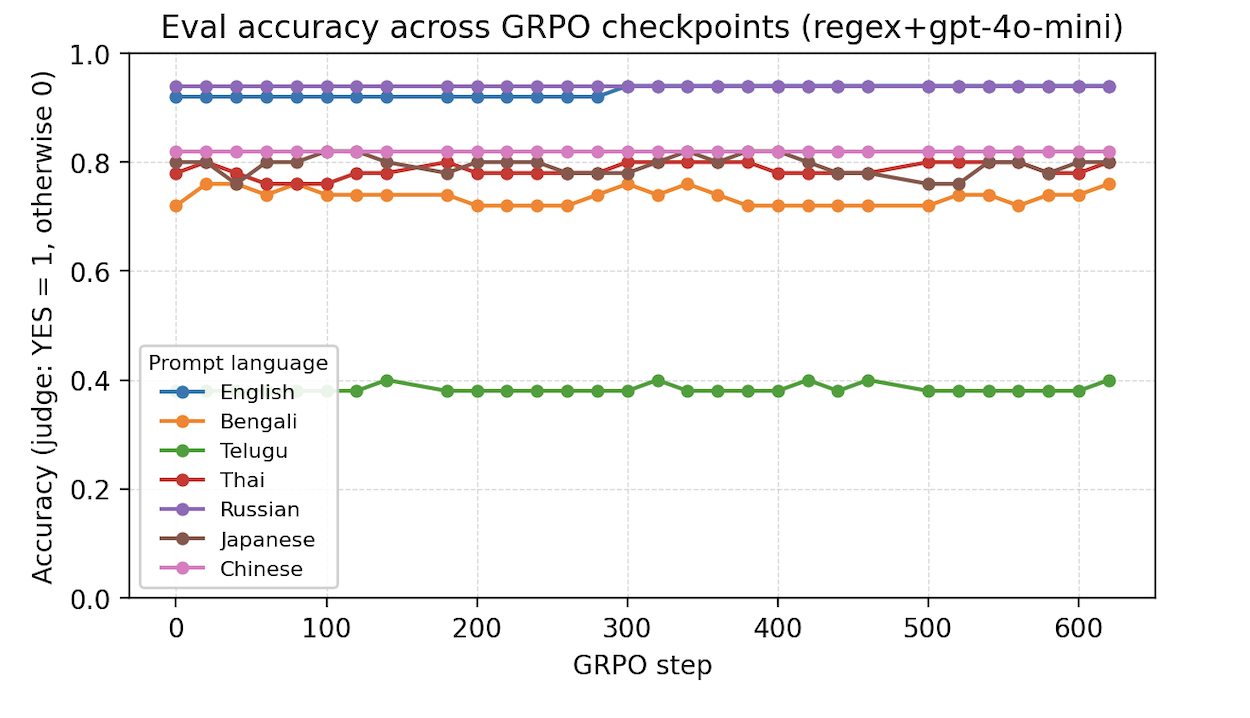
\includegraphics[width=0.8\linewidth]{Chapters/Chapter_4/accuracy_gpt.png}
	\caption{Per-language evaluation accuracy across GRPO training steps, scored by
		the regex-plus-judge verifier. Six languages stay in a band between about $0.72$ and $0.94$ with
		little change over training; Telugu stays at about $0.38$ to $0.40$ throughout.}
	\label{fig:grpo-accuracy}
\end{figure}

% TABLE 4.3 (accuracy first vs last). Booktabs. Label: tab:grpo-acc
\begin{table}[t]
	\centering
	\renewcommand{\arraystretch}{1.2}
	\begin{tabular}{lccc}
		\toprule
		\textbf{Language} & \textbf{Step 0} & \textbf{Step 620} & \textbf{Change} \\
		\midrule
		English  & 0.92 & 0.94 & $+0.02$ \\
		Russian  & 0.94 & 0.94 & $+0.00$ \\
		Chinese  & 0.82 & 0.82 & $+0.00$ \\
		Japanese & 0.80 & 0.80 & $+0.00$ \\
		Thai     & 0.78 & 0.80 & $+0.02$ \\
		Bengali  & 0.72 & 0.76 & $+0.04$ \\
		Telugu   & 0.38 & 0.40 & $+0.02$ \\
		\bottomrule
	\end{tabular}
	\caption{Evaluation accuracy at the first and last checkpoint. The changes are
		small for every language, and Telugu stays far below the rest.}
	\label{tab:grpo-acc}
\end{table}

\subsection{Which Language Does the Model Predict in at Each Layer?}
\label{subsec:grpo-logitlens}

Figure~\ref{fig:grpo-logitlens} shows, by layer and by training step, how much of the
model's logit-lens prediction mass falls on each language, renormalized over the
seven studied languages, for a Telugu prompt and a Thai prompt. The pattern is the
same across prompt languages. For a non-English prompt, the early and middle layers
put most of their renormalized mass on English, with the prompt's own language near
zero, and the target language appears only in the last two or three layers, where
English is still comparable to it. So the model reads out as English through the body
of the stack and surfaces the target language only at the very end.

For this chapter the important thing is how this changes with training, which is to
say it does not. Across all $620$ GRPO steps the per-layer pattern is flat: the
English mass in the early and middle layers does not grow, and the point at which the
target language appears does not move. GRPO does not build up the English-leaning
middle of the stack, and it does not remove it. This holds for every language.

% FIGURE 4.2 -- include here.
% PLOT: from plots/plot1/. Recommended: a small grid of layer-vs-checkpoint heatmaps
% for the low-resource case, e.g. plot1_heatmap_prompt-te_target-en.png and
% plot1_heatmap_prompt-te_target-te.png, to show English high through the body and
% Telugu near zero until the top. Optionally add a high-resource case for contrast.
% Suggested filename: fig_grpo_logitlens.png
\begin{figure}[ht]
	\centering
	 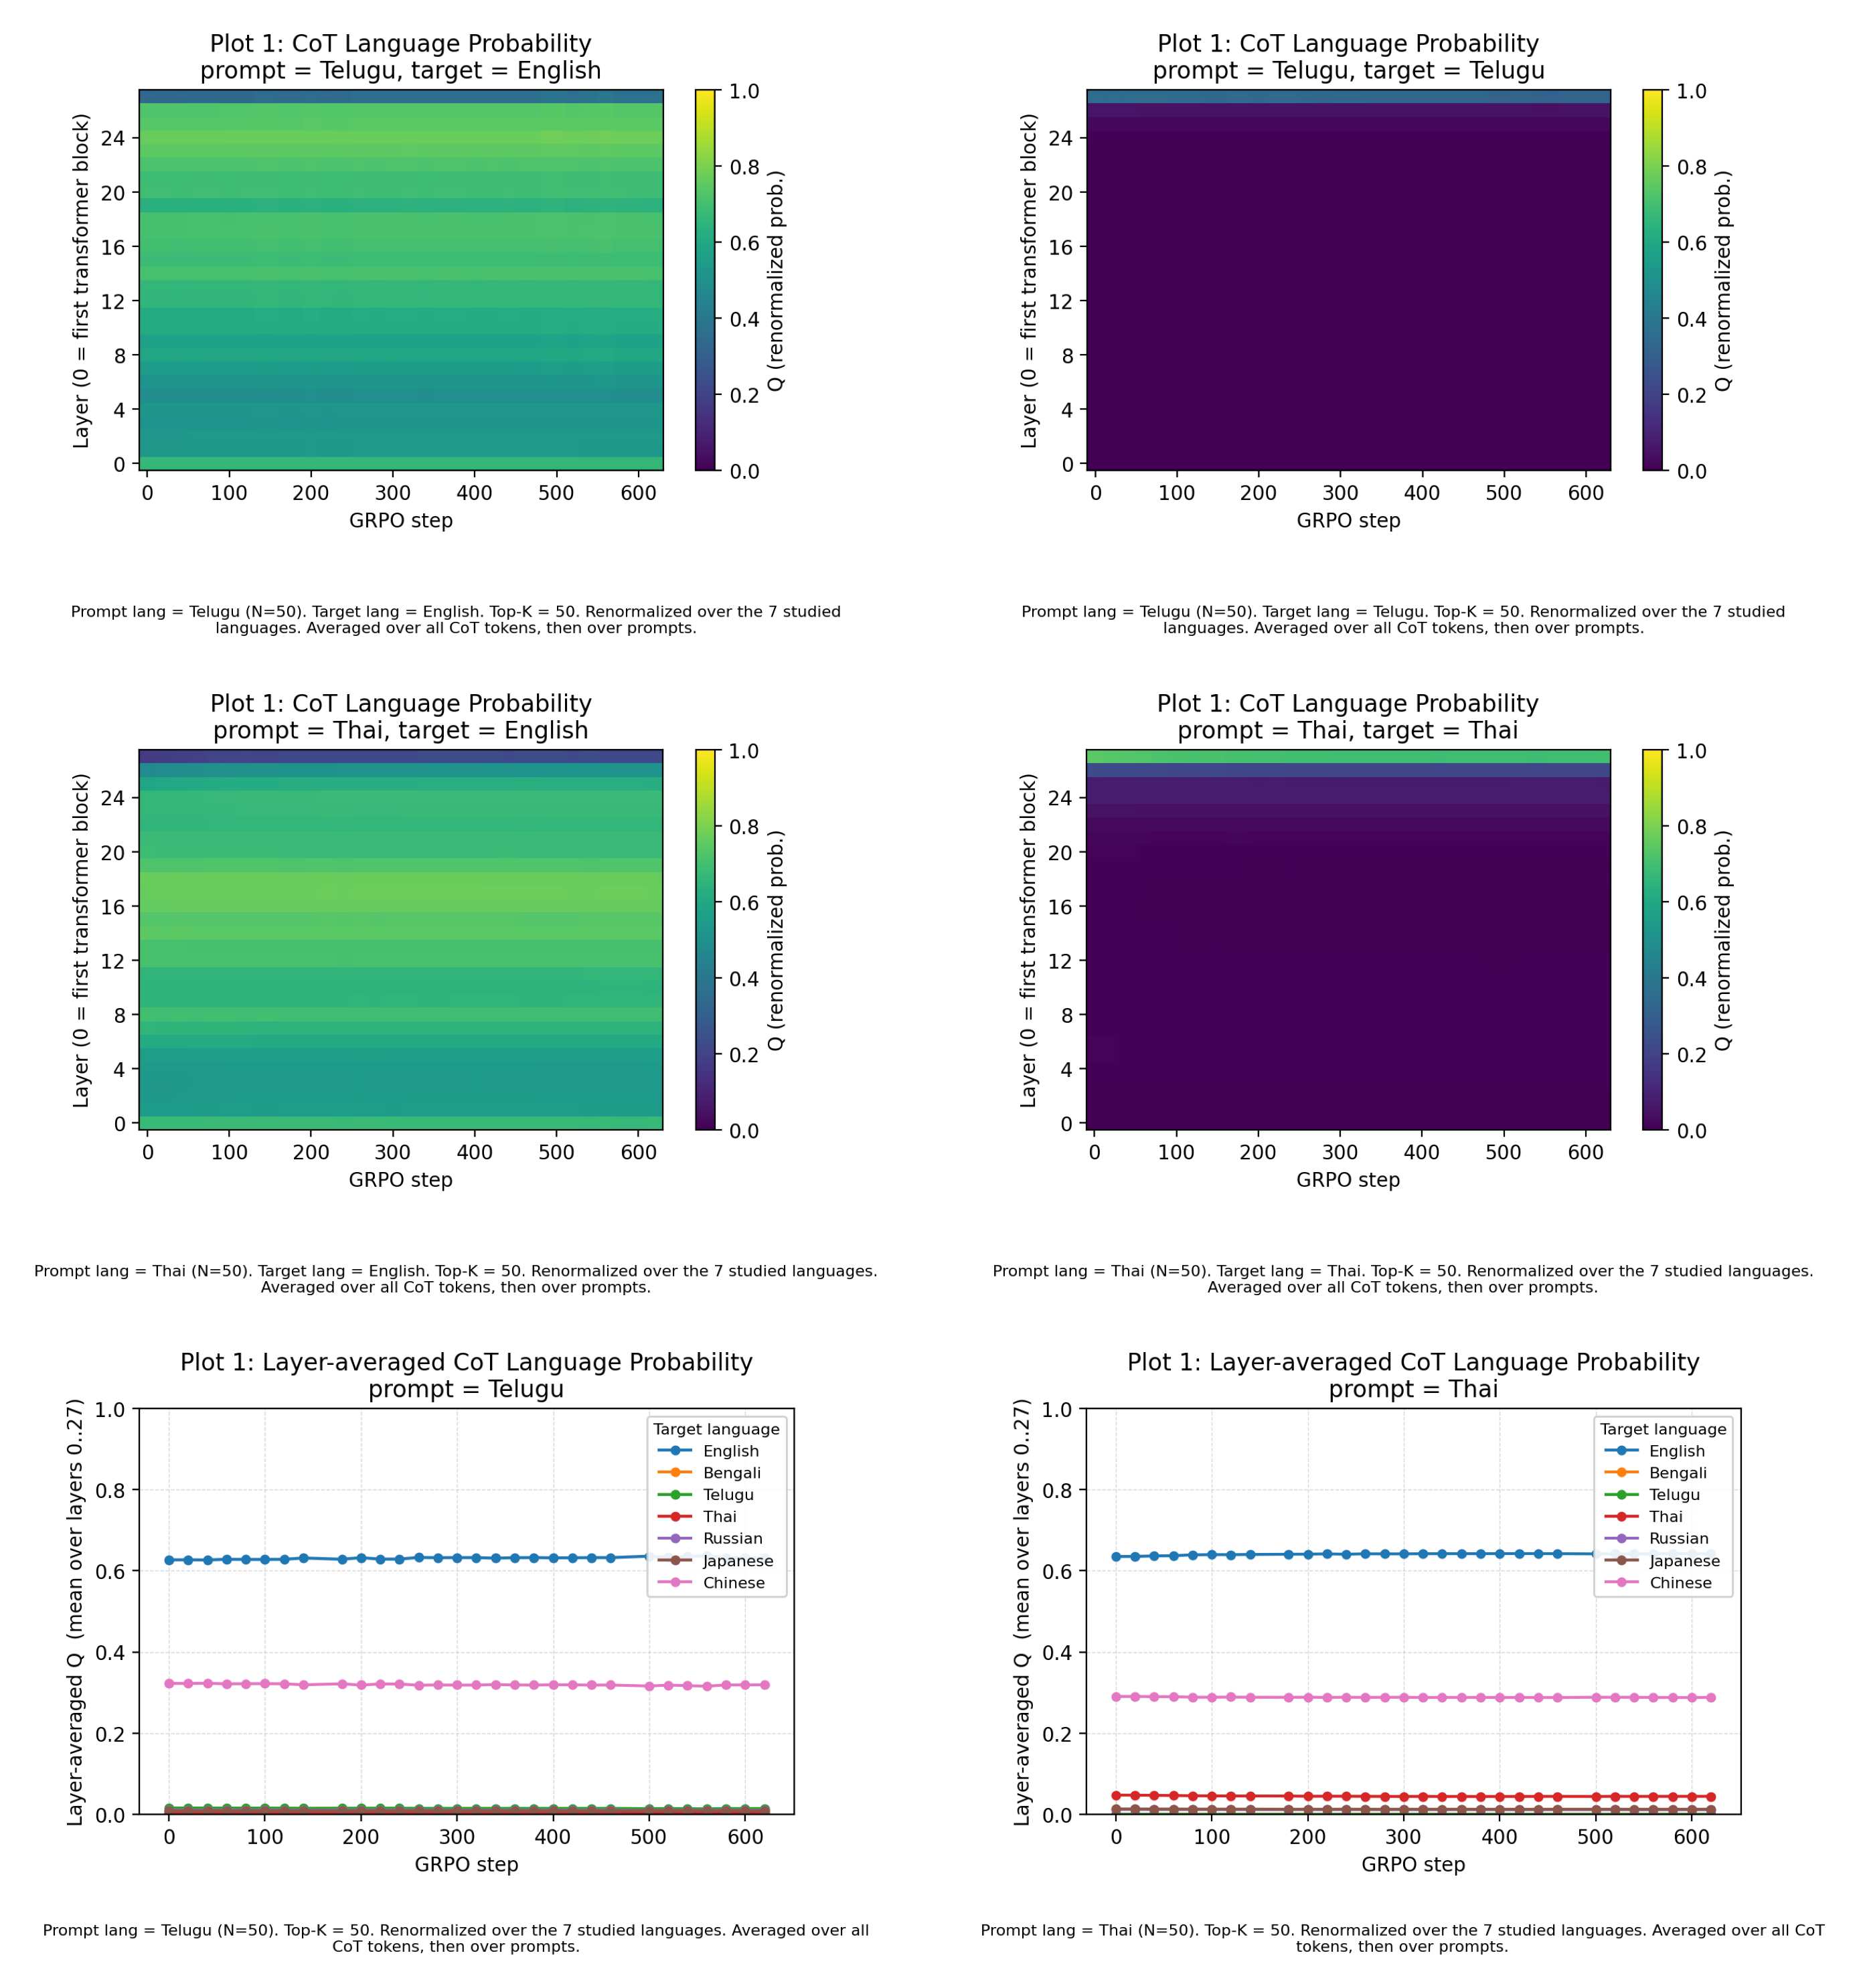
\includegraphics[width=0.8\linewidth]{Chapters/Chapter_4/Figures/combined_plot1.png}
	\caption{Logit-lens language probability for a Telugu prompt (left column) and a
		Thai prompt (right column). The top row is the renormalized probability of an
		English readout, by layer (vertical) and GRPO step (horizontal). The middle row is
		the same for the prompt's own-language readout. The bottom row averages the
		probability over layers and plots it against GRPO step, with one curve per target
		language. For both prompts, English probability is high through the early and middle
		layers while the prompt's own language stays near zero until the last two or three
		layers. All panels are flat across training, so GRPO does not change this pattern.}
	\label{fig:grpo-logitlens}
\end{figure}

\subsection{Three-Phase Analysis and the English Lead}
\label{subsec:grpo-threephase}

Figure~\ref{fig:grpo-threephase} gives the coarser categorical view, the fraction of
layers in each phase whose top-1 logit-lens prediction is a token of a given language,
together with the same at the last few layers. It confirms the picture above. English
is the most common top-1 prediction in the early and middle phases, with its share
highest in the middle phase. The target language appears mainly in the late phase, and
the two prompts differ at the very end: for Thai the target rises clearly at the last
layer and overtakes English, while for Telugu it stays low throughout.

Figure~\ref{fig:grpo-gap} states the same thing as one number per layer: the gap
between the English fraction and the target fraction of top-1 predictions. The gap is
positive through the early and middle layers for both prompts, meaning English leads
there. It is largest in the middle layers, around $0.55$ to $0.62$, and smaller in the
early and late layers. At the very end the two prompts differ: for Telugu the gap stays
positive, so English keeps the lead, while for Thai the gap turns negative at the last
layer, where Thai overtakes English. As with the other measurements, the gap is flat
across the $620$ steps, so GRPO does not change it.

% FIGURE 4.3 -- include here.
% PLOT: from plots/plot2/. Use plot2_lineplot_prompt-te.png (low-resource case),
% optionally beside plot2_lineplot_prompt-th.png.
% Suggested filename: fig_grpo_threephase.png
\begin{figure}[ht]
	\centering
	 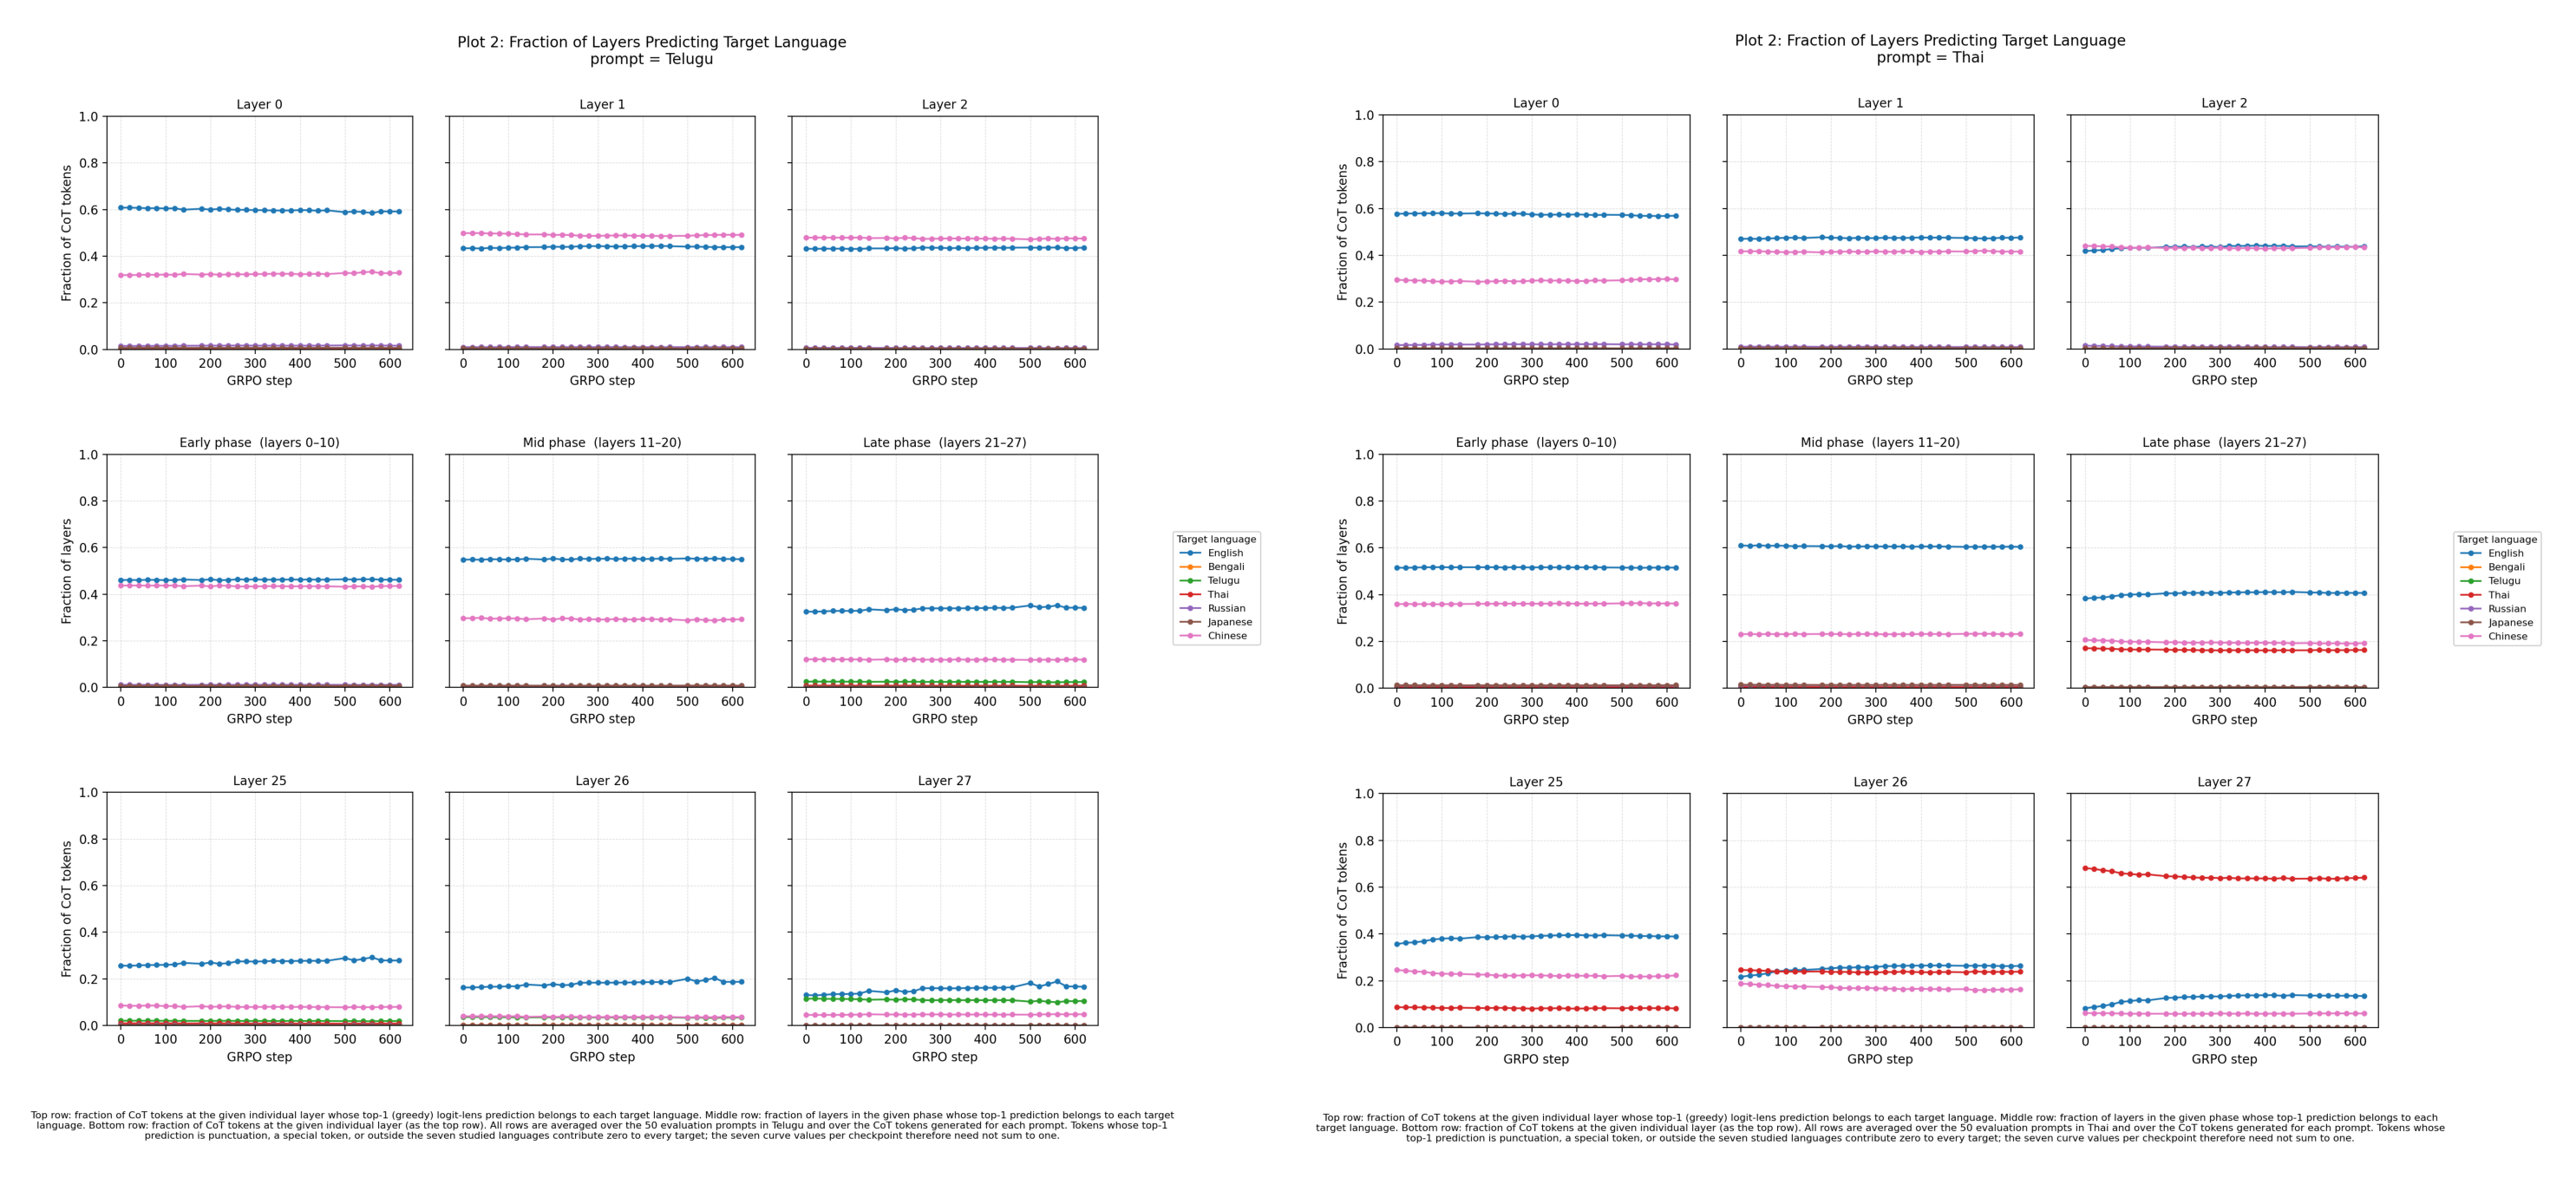
\includegraphics[width=\linewidth]{Chapters/Chapter_4/Figures/combined_plot2.png}
	\caption{Fraction of top-1 logit-lens predictions belonging to each target
		language, across GRPO steps, for a Telugu prompt (left block) and a Thai prompt
		(right block). Within each block, the top row is the first few individual layers,
		the middle row is the early, middle, and late phases, and the bottom row is the
		last few individual layers. English leads the early and middle phases for both
		prompts. The target language appears only in the late phase and final layers: for
		Thai it rises clearly at the last layer, while for Telugu it stays low throughout.
		The curves do not change over training.}
	\label{fig:grpo-threephase}
\end{figure}

% FIGURE 4.4 -- include here.
% PLOT: from plots/plot2_gap/. Use plot2_gap_lineplot_prompt-te.png, optionally beside
% another language. (This is the English-minus-target gap per phase / per layer.)
% Suggested filename: fig_grpo_gap.png
\begin{figure}[ht]
	\centering
	 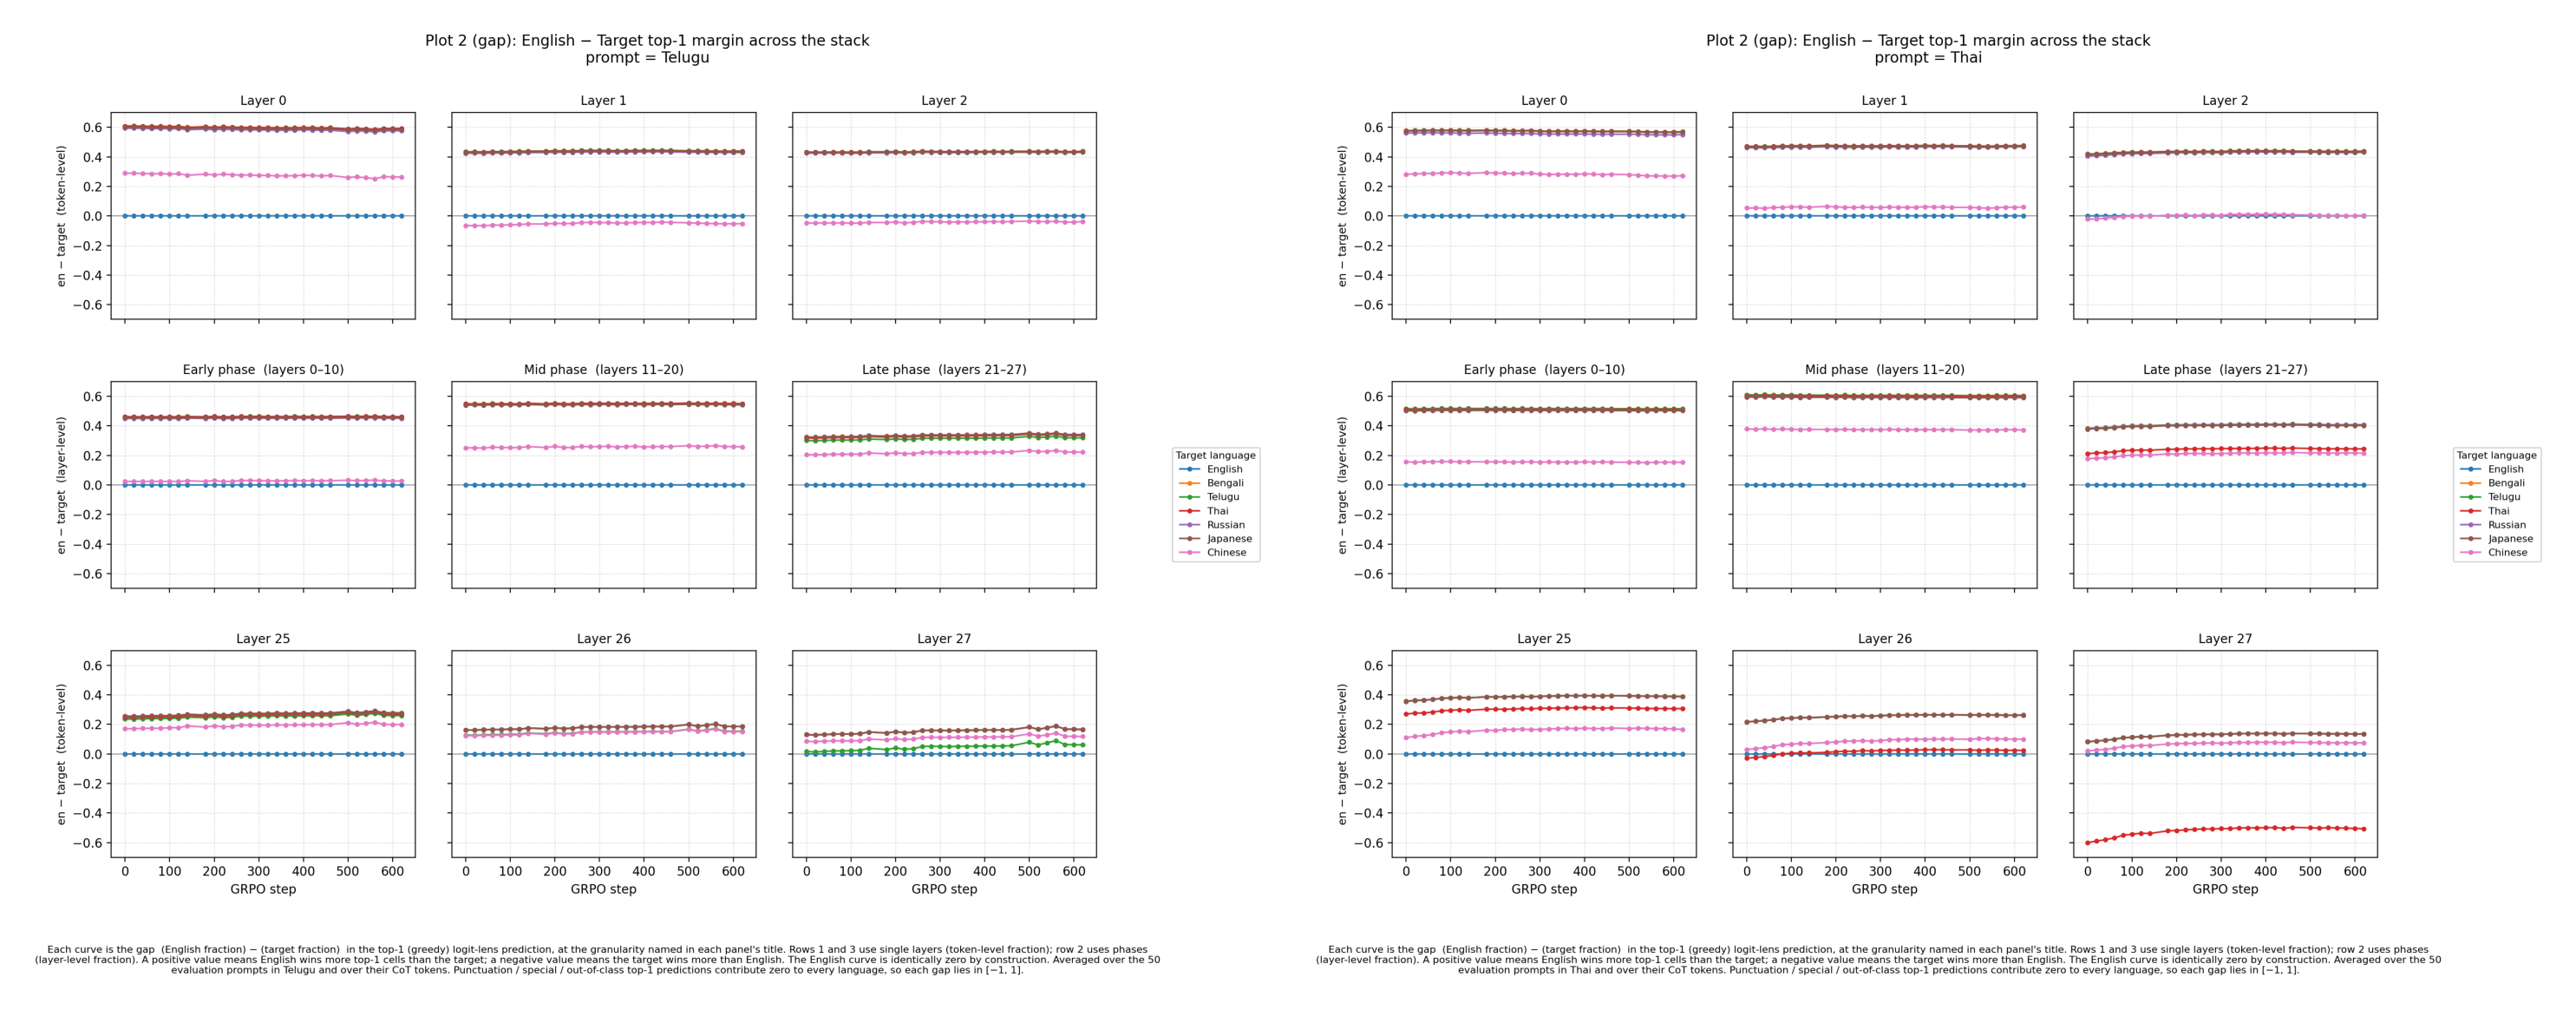
\includegraphics[width=\linewidth]{Chapters/Chapter_4/Figures/combined_plot2_gap.png}
	\caption{Gap between the English fraction and the target fraction of top-1
		logit-lens predictions, across GRPO steps, for a Telugu prompt (left block) and a
		Thai prompt (right block). A positive gap means English wins more top-1 predictions
		than the target language; a negative gap means the target wins. Within each block,
		the top row is the first few individual layers, the middle row is the early,
		middle, and late phases, and the bottom row is the last few individual layers. The
		gap is positive through the early and middle layers for both prompts, so English
		leads there. At the final layers the two prompts differ: for Thai the gap turns
		negative at the last layer, where Thai overtakes English, while for Telugu it stays
		positive throughout. The curves do not change over training.}
	\label{fig:grpo-gap}
\end{figure}

\subsection{Representation Geometry}
\label{subsec:grpo-geometry}

The measurements so far show that GRPO does not change the model's per-layer language
behaviour. The last one shows where its effect does appear, and it singles out
Telugu. Figure~\ref{fig:grpo-cka} shows two CKA measurements.

The cross-lingual similarity (left) compares each language's representations with
English, layer-averaged, across training. The curves are flat over the $620$ steps,
so training does not pull the languages closer to or further from English in
representation space. They differ by language in a way that tracks coverage: the two
low-coverage Indic languages, Telugu and Bengali, are least similar to English (around
$0.10$ and $0.15$), Russian is in the middle (around $0.32$), and Thai, Japanese, and
Chinese are highest (around $0.40$).

The within-language drift (right) compares each language at a checkpoint with the same
language at step $0$, so a lower value means training has moved it more. Telugu stands
out. Every other language stays above about $0.90$ for the whole run, meaning their
representations barely move. Telugu drops well below the rest, reaching about $0.63$ at
its lowest before settling near $0.78$. So the one language that sits far below the
others in accuracy, and does not improve, is also the one whose representations GRPO
disturbs the most. The training signal is clearly reaching Telugu and changing its
representations; it is just not turning into any accuracy gain.

% FIGURE 4.5 -- include here.
% PLOT: plots/plot4/plot4_lineplot.png (cross-lingual CKA vs English) and
% plots/plot4/plot4_drift_lineplot.png (within-language drift vs step 0), side by side.
% Suggested filename: fig_grpo_cka.png
\begin{figure}[ht]
	\centering
	 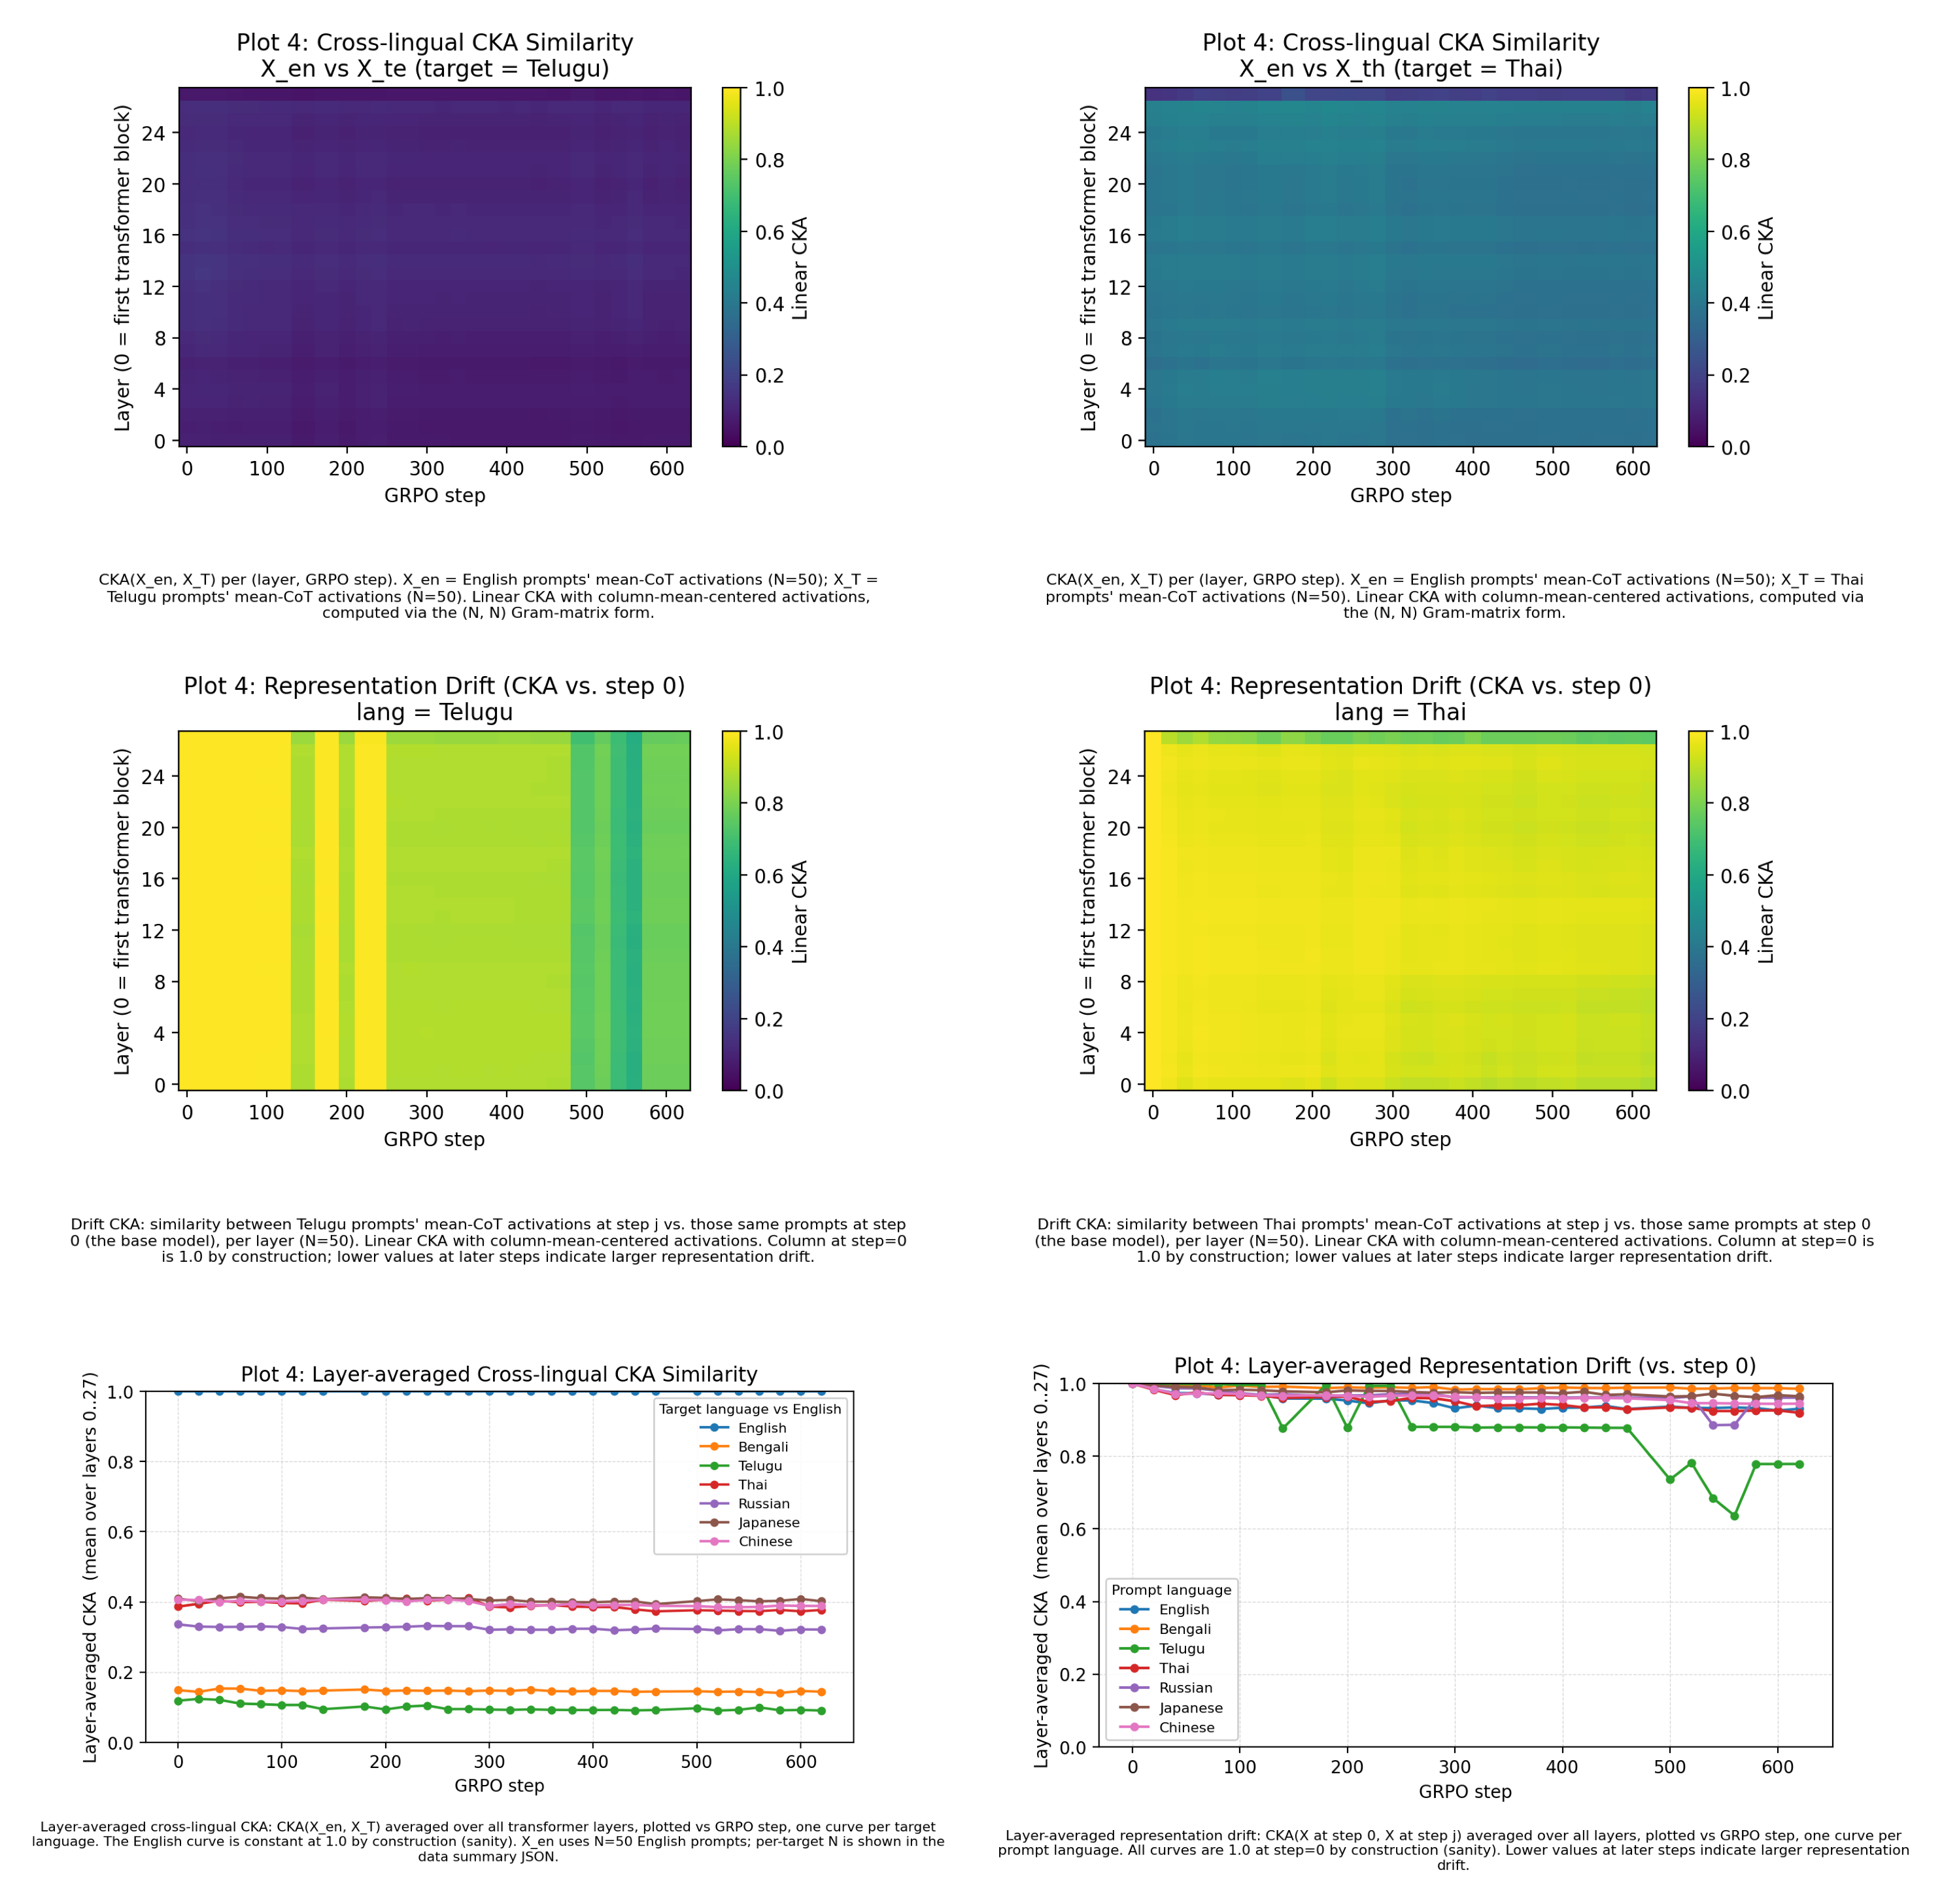
\includegraphics[width=0.8\linewidth]{Chapters/Chapter_4/Figures/combined_plot4.png}
	\caption{Representation similarity measured with CKA, across GRPO steps. The top
		row is the cross-lingual similarity between each prompt language and English, by
		layer (vertical) and GRPO step (horizontal), for Telugu (left) and Thai (right);
		Thai is more similar to English than Telugu at every layer. The middle row is the
		within-language drift, the similarity between a language's representations at a
		given step and at step $0$, for Telugu (left) and Thai (right); a lower value means
		training has moved the representations more. The bottom row gives the
		layer-averaged versions across all languages: cross-lingual similarity to English
		(left) and within-language drift (right). The low-coverage Indic languages, Telugu
		and Bengali, are least similar to English, and Telugu drifts the most over
		training, while every other language barely moves. All curves are flat in the
		cross-lingual similarity, so training does not change how close the languages sit
		to English.}
	\label{fig:grpo-cka}
\end{figure}

\section{Discussion}
\label{sec:grpo-discussion}

\subsection{GRPO Does Not Cause Cross-Lingual Collapse}
\label{subsec:grpo-no-collapse}

We set out to test whether GRPO, by rewarding only the final answer, pushes the model
toward an English-aligned middle of the stack and widens the gap for low-resource
languages over training. The results do not support this. The model does read out as
English through the early and middle layers and surfaces the target language only at
the end, which matches the static three-phase picture, but this is already present in
the base model at step $0$ and does not change over $620$ GRPO steps. The per-layer
distribution, the three-phase commitment, and the English-minus-target gap are all
flat in training. GRPO does not build up the English-leaning middle, and it does not
collapse the low-resource languages into it. Whatever that part of the stack is doing,
GRPO leaves it as it was.

\subsection{Tokeniser Coverage and the Telugu Case}
\label{subsec:grpo-coverage-discussion}

If GRPO is not changing the internal routing, what sets Telugu apart? Telugu sits far
below every other language in accuracy and does not improve, and it is also the one
whose representations GRPO moves the most. The geometry points to coverage: Telugu and
Bengali, the two languages with the fewest dedicated tokens, are the least similar to
English in representation space, and Telugu, with only about $14$ tokens, is the one
that drifts most while gaining nothing.

The reading we draw is that the limiting factor for GRPO here is the granularity of
the reward signal it can act on. When a language has very few dedicated tokens, its
text is broken into long, coarse byte sequences, and the reward, which depends on
producing a correct final answer, cannot be turned into a useful per-token gradient.
Training still moves the representations, as the Telugu drift shows, but the movement
does not line up with task competence, so the accuracy does not move. The relevant
variable is therefore coverage, not language identity and not a change in the model's
internal routing.


\section{Limitations}
\label{sec:grpo-limitations}

This study has several limitations. It uses one model family, Qwen2.5-7B-Instruct,
and one task, multilingual grade-school math, so the findings may not carry over to
other models or tasks. The fine-tuning uses a low-rank adapter on the attention
projections only, not full fine-tuning, which may limit how much the model can change.
The logit-lens readout assumes that applying the final head to an intermediate layer
is meaningful, which is a standard but imperfect assumption. The reward depends on a
verifier that combines a regex match with a judge model, which can make mistakes. The
tokeniser-coverage counts are approximate, based on script ranges in the vocabulary.
Finally, the study covers seven languages, so the coverage pattern we describe is a
pattern across these languages rather than a precisely located cutoff.

 
\chapter{Group Robust Preference Optimization in the Multi-Label Setting}
\label{ch:fairpo}

\section{Introduction}
\label{sec:fairpo-intro}

\subsection{Motivation}
\label{subsec:fairpo-motivation}

In multi-label classification a single input can carry several labels at once, and
a model predicts each of them. The usual way to train such a model is to minimize
one aggregate loss summed over all labels, which treats every label as equally
important \citep{kiritchenko2006hierarchical, schietgat2010predicting}. The labels
are rarely equal in practice. Some are rare, so their training signal is small next
to the frequent ones \citep{charte2015imbalance}. Some matter more than others,
such as a rare disease against a common finding
\citep{rajpurkar2017chexnetradiologistlevelpneumoniadetection}. And some are simply
harder to tell apart from a close alternative. With an aggregate loss, the easy and
frequent labels take over training, and the labels that matter most are often the
ones the model handles worst.

The standard fixes do not close this gap. Binary cross-entropy scores each label on
its own, so the signal for a rare label is easily drowned out by the frequent ones
\citep{bce_loss, charte2015imbalance}. Focal Loss down-weights easy examples,
but it still scores each label in isolation \citep{lin2018focal}.
None of these teaches the model to separate a true label from the specific
incorrect label it is being confused with. What is missing is an objective that can
express a preference between two labels, so that the model learns to score a true
label above the competitor most likely to be mistaken for it. This is the gap the
chapter addresses.

This chapter also fits the larger argument of the thesis. The earlier chapters
showed that acting on a localized part of a model does not reliably change its
behaviour, and that the training objective is the more effective place to work.
Here we follow that idea in a different setting. Rather than analysing an objective,
we design one: an objective that improves a chosen group of labels while protecting
the rest.

\subsection{Problem Statement}
\label{subsec:fairpo-problem}

We study how to improve a model on a chosen subset of labels without degrading the
others. Concretely, we split the label set into a privileged group, which we want
to improve, and a non-privileged group, whose performance we want to keep at a
baseline level, and we ask for a training objective that handles both at once. This
breaks into three parts.

\begin{enumerate}
	\item \textbf{How to improve the privileged labels.} The difficulty for these
	labels is usually fine-grained discrimination against a close, incorrect
	alternative, which a point-wise loss does not target. We need an objective that
	acts on pairs of labels and prefers the true one over its confusing competitor.
	
	\item \textbf{How to protect the non-privileged labels.} Improving one group
	should not come at the cost of the rest. We need an objective for the
	non-privileged group that allows learning to focus elsewhere but steps in when
	a label starts to drop below a reliable baseline.
	
	\item \textbf{How to balance the two.} The two objectives compete, and a fixed
	weighted sum does not adapt as training proceeds. We need a way to balance them
	that shifts focus to whichever group is currently doing worse.
\end{enumerate}

\subsection{Contributions}
\label{subsec:fairpo-contributions}

This chapter, based on our published work \citep{mondal2025fairpo}, reports the
following.

\begin{itemize}
	\item We propose FairPO, a framework for multi-label classification that
	partitions the labels into a privileged group and a non-privileged group and
	applies a different objective to each: a preference-based objective for the
	privileged group and a constrained objective for the non-privileged group.
	
	\item We adapt preference optimization, which was developed for aligning
	generative models, to a discriminative classification task. For a privileged
	label, FairPO finds the incorrect labels that are scored too close to it and
	trains the model to prefer the true label over them. We give three variants,
	based on DPO \citep{rafailov2023direct}, CPO \citep{xu2024contrastive}, and SimPO
	\citep{meng2024simpo}.
	
	\item We balance the two group objectives with a Group Robust Preference
	Optimization formulation \citep{ramesh2024group}, set up as a minimax problem
	over the two label groups, which is a new use of this method in this setting.
\end{itemize}

On MS-COCO and NUS-WIDE, FairPO improves accuracy on the rare privileged labels, by
up to $+3.44$ $\Delta\text{mAP}$ over the BCE-SFT baseline with its CPO variant,
while leaving the frequent labels almost unchanged, and it does better than the
baselines we compare against.

\section{The FairPO Framework}
\label{sec:fairpo-framework}

\subsection{Problem Setup}
\label{subsec:fairpo-setup}

We work in a standard multi-label classification setting with a dataset
$\dataset = \{ (\mathbf{x}_i, y_i) \}_{i=1}^N$, where $\mathbf{x}_i$ is an input and
$y_i \in \{0, 1\}^{|\labels|}$ is its label vector over a set of $|\labels|$
labels. We train a model with parameters $\params$ that gives a per-label score
$\model(\mathbf{x}_i; \params_t)$ for each label $t \in \labels$. The framework
also uses a fixed reference model with parameters $\refparams_t$, which in our
experiments is a model trained with binary cross-entropy.

The idea behind FairPO is to split the label set $\labels$ into two disjoint
groups:
\begin{itemize}
	\item a \emph{privileged} group $\privileged \subset \labels$, the labels we
	want to improve, and
	\item a \emph{non-privileged} group $\nonprivileged = \labels \setminus
	\privileged$, the remaining labels, whose performance we want to keep at least
	at a baseline level.
\end{itemize}
How the labels are assigned to the two groups is left open and can be chosen for
the problem, for example by label frequency for class imbalance, or by domain
importance. In this chapter we use class imbalance, so the privileged group is the
set of least frequent labels. The exact partition is given in
Section~\ref{subsec:fairpo-data}.

Figure~\ref{fig:fairpo-overview} gives an overview of the framework: each sampled
label is routed to a privileged or non-privileged path with its own objective, and
a group-robust step balances the two.

% FIGURE 5.1 -- include the FairPO framework diagram here.
% Suggested filename: fig_fairpo_method.pdf (the paper's Figure 1 / method.pdf)
\begin{figure}[ht]
	\centering
	 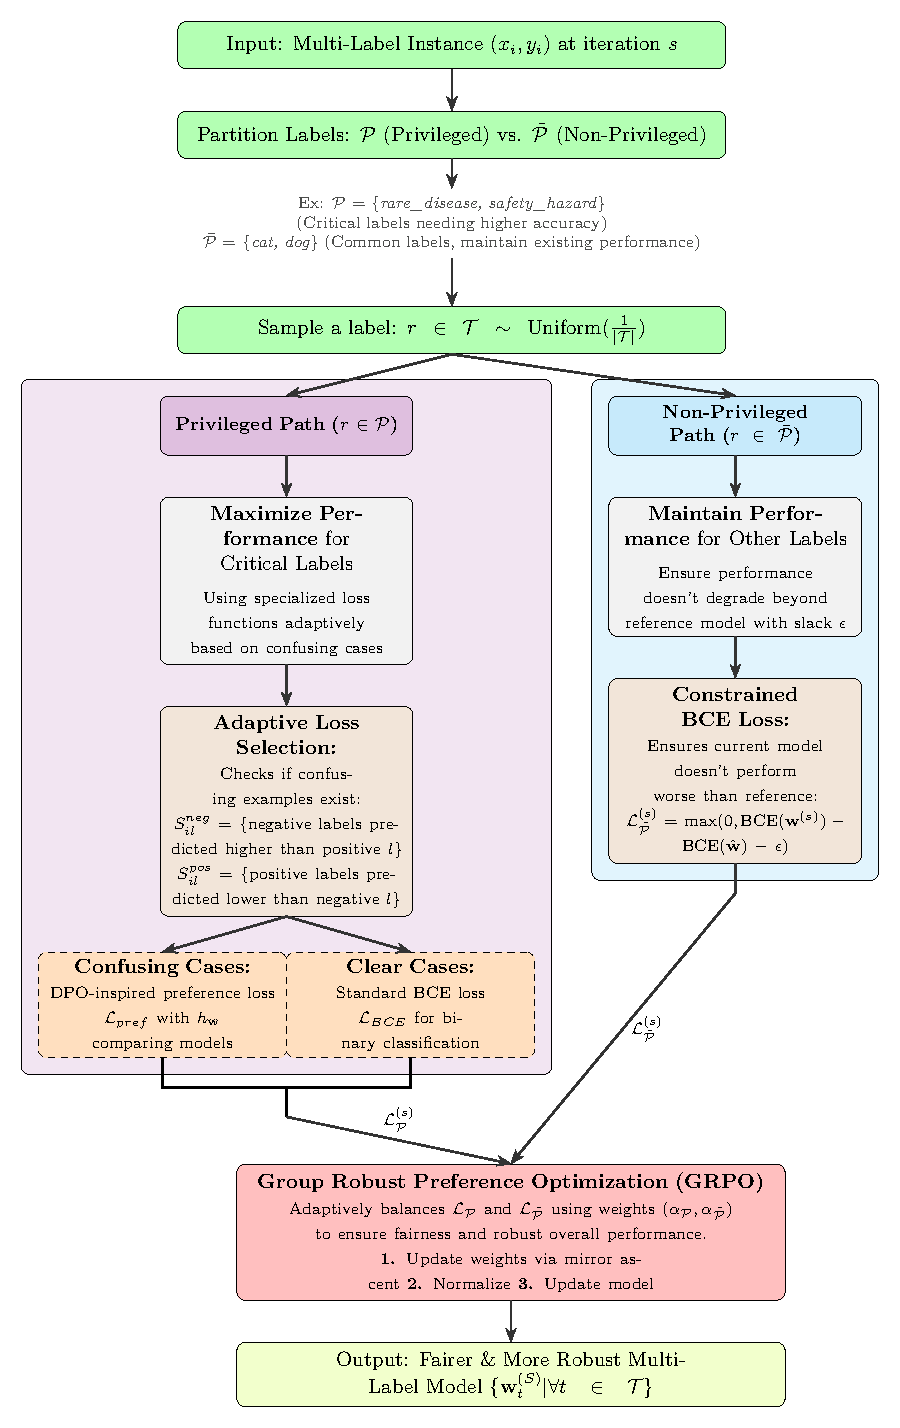
\includegraphics[width=0.5\linewidth]{Chapters/Chapter_5/method.pdf}
	\caption{Overview of the FairPO framework. Labels are partitioned into a
		privileged group and a non-privileged group. A sampled label is routed to the
		privileged path, which uses a preference loss with a BCE fallback, or the
		non-privileged path, which uses a constrained BCE loss against a reference
		model. A Group Robust Preference Optimization step balances the two group
		losses.}
	\label{fig:fairpo-overview}
\end{figure}

\subsection{Objective for the Privileged Group}
\label{subsec:fairpo-privileged}

For the privileged group, reweighting a standard loss is not enough. The main
difficulty for these labels is usually not basic classification but telling a label
apart from a close, incorrect alternative. We therefore set up the objective for
this group as a preference learning task.

\paragraph{Confusing counterparts.}
For an instance $\mathbf{x}_i$ and a privileged label $l \in \privileged$, we
identify a set of confusing counterparts from the model's current scores. There are
two cases. When the true label is positive ($y_{il}=1$), the confusing negatives
are the incorrect labels that the model scores at least as high as the true label:
\begin{equation}
	S_{il}^{\text{neg}} = \{k \in \labels \mid y_{ik}=0 \text{ and } \model(\mathbf{x}_i; \params_k) \ge \model(\mathbf{x}_i; \params_l) \}.
	\label{eq:fairpo-confusing-neg}
\end{equation}
When the true label is negative ($y_{il}=0$), the confusing positives are the
correct labels that the model scores no higher than the true negative:
\begin{equation}
	S_{il}^{\text{pos}} = \{k \in \labels \mid y_{ik}=1 \text{ and } \model(\mathbf{x}_i; \params_k) \le \model(\mathbf{x}_i; \params_l) \}.
	\label{eq:fairpo-confusing-pos}
\end{equation}
The full confusing set for $(i, l)$ is $\confusing = S_{il}^{\text{neg}} \cup S_{il}^{\text{pos}}$.

\paragraph{Conditional objective with a fallback.}
The objective for the privileged group is adaptive. When $\confusing$ is non-empty,
we apply a preference loss $\loss_{\text{pref}}$ to the hard discriminative case.
As the model improves, the confusing set for many instances becomes empty, and a
preference loss alone would then give a sparse gradient and stall training. To keep
a learning signal, we fall back to a standard binary cross-entropy loss when
$\confusing = \emptyset$:
\begin{equation}
	\baseloss_{\text{BCE}}(\mathbf{x}_i, y_{il}; \params_l) = -[y_{il} \log \model(\mathbf{x}_i; \params_l) + (1-y_{il}) \log(1-\model(\mathbf{x}_i; \params_l))].
	\label{eq:fairpo-bce}
\end{equation}
Early in training the model makes many mistakes, the confusing sets are large, and
the preference loss is used often. As the preference loss resolves these cases, the
fallback takes over and fine-tunes the easier examples. The total privileged loss
$\loss_{\privileged}$ is the expectation over this conditional choice.

\paragraph{DPO variant.}
To write the preference losses in one form, let $\model(\mathbf{x}_i; \params_p)$
be the score of the preferred label in a pair and
$\model(\mathbf{x}_i; \params_d)$ the score of the dispreferred label. The roles
follow the ground truth: if $y_{il}=1$ and $k \in S_{il}^{\text{neg}}$, then the
true label is preferred ($p=l$) and the confusing negative is dispreferred
($d=k$); if $y_{il}=0$ and $k \in S_{il}^{\text{pos}}$, then the true negative is
preferred ($p=l$) and the confusing positive is dispreferred ($d=k$). Following DPO
\citep{rafailov2023direct}, the preference loss is taken relative to the reference
model:
\begin{equation}
	\loss_{\text{pref}}^{\text{DPO}}(\mathbf{x}_i, p, d) = -\log \sigma \left( \beta \left( \log \frac{\model(\mathbf{x}_i; \params_p)}{\model(\mathbf{x}_i; \refparams_p)} - \log \frac{\model(\mathbf{x}_i; \params_d)}{\model(\mathbf{x}_i; \refparams_d)} \right) \right).
	\label{eq:fairpo-dpo-pref}
\end{equation}
The full DPO-based privileged loss combines this with the fallback:
\begin{align}
	\loss_{\privileged}^{\text{DPO}} = \E_{(\mathbf{x}_i,l) \text{ s.t. } l \in \privileged}
	\left[
	\mathbf{1}_{\confusing \neq \emptyset} \cdot \loss_{\text{pref}}^{\text{DPO}}(\mathbf{x}_i, p, d) + \mathbf{1}_{\confusing = \emptyset} \cdot \baseloss_{\text{BCE}}(\mathbf{x}_i, y_{il}; \params_l)
	\right],
	\label{eq:fairpo-dpo-combined}
\end{align}
where for a sampled privileged label $l$ with a non-empty confusing set, a
counterpart $k$ is sampled from $\confusing$ and the pair $(p,d)$ is set from
$(l,k)$ and the ground truth.

\paragraph{SimPO variant.}
This variant adapts SimPO \citep{meng2024simpo} to give
a reference-free preference loss with a target margin $\gamma > 0$, applied to the
per-label scores:
\begin{equation}
	\loss_{\text{pref}}^{\text{SimPO}}(\mathbf{x}_i, p, d) = -\log \sigma \left( \beta \log \frac{\model(\mathbf{x}_i; \params_p)}{\model(\mathbf{x}_i; \params_d)} - \gamma \right).
	\label{eq:fairpo-simpo-pref}
\end{equation}
The log-ratio term measures the relative preference, and the margin $-\gamma$ pushes
the model to separate the two scores by a set amount rather than only rank them
correctly. This term replaces the DPO term in the conditional objective of
Equation~\ref{eq:fairpo-dpo-combined}.

\paragraph{CPO variant.}
The last variant adapts CPO \citep{xu2024contrastive},
which is reference-free and adds a BCE regularizer to the preference term. When a
confusing set exists, the loss is
\begin{equation}
	\loss_{\text{pref}}^{\text{CPO}}(\mathbf{x}_i, p, d, l) = -\log \sigma \left( \beta \log \frac{\model(\mathbf{x}_i; \params_p)}{\model(\mathbf{x}_i; \params_d)} \right) + \lambda_{\text{CPO}} \cdot \baseloss_{\text{BCE}}(\mathbf{x}_i, y_{il}; \params_l).
	\label{eq:fairpo-cpo-pref}
\end{equation}
The first term is a margin-free preference objective, and the second, weighted by
$\lambda_{\text{CPO}}$, is the BCE loss for the privileged label $l$, which keeps
the model grounded in absolute scores. As in the DPO case, this loss is used when a
confusing set is found, and the BCE fallback of Equation~\ref{eq:fairpo-bce} is used
otherwise.

The reason for using a preference loss at all is that point-wise losses like BCE
and Focal Loss score each label on its own. They answer whether a label's score is
right in isolation, which gives only a weak signal when a true label at $0.8$ sits
just above a confusing label at $0.7$. The preference loss instead asks whether the
true label is scored clearly above its specific competitor, and the log-ratio gives
a direct gradient that pushes the two scores apart.

\subsection{Objective for the Non-Privileged Group}
\label{subsec:fairpo-nonprivileged}

For the non-privileged group the goal is not to push performance up but to keep it
from dropping. We use a constrained objective against the reference model. For a
label $j \in \nonprivileged$ we take the BCE loss of
Equation~\ref{eq:fairpo-bce}, and we penalize the model only when its loss is worse
than the reference model's loss by more than a slack margin $\epsilon \ge 0$,
through a hinge:
\begin{equation}
	\loss_{\nonprivileged} = \E_{(\mathbf{x}_i,j) \text{ s.t. } j \in \nonprivileged} \left[ \max(0, \baseloss_{\text{BCE}}(\mathbf{x}_i, y_{ij}; \params_j) - \baseloss_{\text{BCE}}(\mathbf{x}_i, y_{ij}; \refparams_j) - \epsilon) \right].
	\label{eq:fairpo-np-constrained}
\end{equation}
The gradient is zero as long as a non-privileged label is doing about as well as
the reference, and a signal appears only when the label drops below that threshold.
This keeps the non-privileged group from degrading while the model spends its
capacity on the privileged group.

\subsection{Group-Robust Balancing}
\label{subsec:fairpo-grpo}

We now have two objectives that pull against each other: the preference-based loss
$\loss_{\privileged}$ for the privileged group and the constrained loss
$\loss_{\nonprivileged}$ for the non-privileged group. A fixed weighted sum of the
two does not handle this well, since the right balance changes during training. We
instead treat the two label groups as the groups in a Group Robust Preference
Optimization problem \citep{ramesh2024group} and write the objective as a minimax
game:
\begin{equation}
	\min_{\{\params_t\}} \max_{\alpha \in \Delta} \left[ \alpha_{\privileged} \loss_{\privileged} + \alpha_{\nonprivileged} \loss_{\nonprivileged} \right],
	\label{eq:fairpo-objective}
\end{equation}
where $\alpha = (\alpha_{\privileged}, \alpha_{\nonprivileged})$ are adaptive
weights on the probability simplex $\Delta$. The inner maximization puts more
weight on whichever group currently has the higher loss, so training focuses on the
worse-off group, and the outer minimization updates the model under that weighting.
This gives a way to manage the trade-off between the two groups rather than fixing
it in advance.

\subsection{Optimization}
\label{subsec:fairpo-optim}

We solve Equation~\ref{eq:fairpo-objective} with alternating mirror ascent on the
weights $\alpha$ and mirror descent on the parameters $\params$, shown in
Algorithm~\ref{alg:fairpo-overview}. One detail matters for stability. The two
group losses can be on different scales, so using their raw values in the mirror
ascent step makes the weight updates unstable. We instead update $\alpha$ from the
change of each group's loss relative to its running average, which keeps the
balancing step stable.

\begin{algorithm}[t]
	\caption{FairPO Training Overview (DPO-inspired)}
	\label{alg:fairpo-overview}
	\begin{algorithmic}[1]
		\State \textbf{Initialize:} Model parameters $\Params^{(0)}$ (e.g., from supervised fine-tuning), group weights $\alpha_{\privileged}^{(0)}, \alpha_{\nonprivileged}^{(0)}$
		\State \textbf{Input:} Dataset $\dataset$, reference parameters $\Refparams$, hyperparameters $\beta, \epsilon, \eta_{\params}, \eta_{\alpha}$.
		\State \textbf{For} each training iteration $s = 0, \dots, S-1$:
		\State \hspace{0.5cm} Sample instance $(x_i, y_i) \sim \dataset$ and a label $r \in \mathcal{T}$.
		\State \hspace{0.5cm} \textbf{If} $r \in \privileged$:
		\State \hspace{1.0cm} Compute privileged loss $\loss_{\privileged}^{(s)}$ for $(x_i, r)$ (Eq.~\ref{eq:fairpo-dpo-combined}, or BCE Eq.~\ref{eq:fairpo-bce}).
		\State \hspace{0.5cm} \textbf{Else if} $r \in \nonprivileged$:
		\State \hspace{1.0cm} Compute non-privileged loss $\loss_{\nonprivileged}^{(s)}$ for $(x_i, r)$ (Eq.~\ref{eq:fairpo-np-constrained}).
		\State \hspace{0.5cm} Update group weights $\alpha^{(s+1)}$ via mirror ascent using $\loss_{\privileged}^{(s)}, \loss_{\nonprivileged}^{(s)}$.
		\State \hspace{0.5cm} Update model parameters $\Params^{(s+1)}$ via mirror descent using the weighted gradients.
		\State \textbf{End For}
		\State \textbf{Return} Optimized parameters $\Params^{(S)}$.
	\end{algorithmic}
\end{algorithm}

For the SimPO and CPO variants the structure is identical; only the preference term
inside the privileged loss changes, to
Equation~\ref{eq:fairpo-simpo-pref} or Equation~\ref{eq:fairpo-cpo-pref}. The
group-robust balancing and the non-privileged handling stay the same.


\section{Experimental Setup}
\label{sec:fairpo-setup}

\subsection{Datasets and Label Partition}
\label{subsec:fairpo-data}

We evaluate FairPO on two multi-label image benchmarks, MS-COCO~2014
\citep{lin2015coco} and NUS-WIDE \citep{chua2009nuswide}.
MS-COCO has 80 object categories, with 82{,}783 training images and 40{,}504
validation images, which we use as the test set. NUS-WIDE has 81 concept labels,
with 161{,}789 training images and 107{,}859 test images under the common split.

To set up the class-imbalance case, we partition the labels by frequency. On each
dataset the privileged group $\privileged$ is the set of 16 least frequent labels,
which is about $20\%$ of the labels, and the non-privileged group
$\nonprivileged$ is the rest, 64 labels on MS-COCO and 65 on NUS-WIDE. This makes
the rare labels the ones we try to improve and the frequent labels the ones we try
to maintain. The partition is one choice; as noted in
Section~\ref{subsec:fairpo-setup}, the framework allows other criteria, such as
domain importance.

\subsection{Model}
\label{subsec:fairpo-model}

The base model is a Vision Transformer, \texttt{vit-base-patch16-224}
\citep{dosovitskiy2021vit}, pre-trained on ImageNet-21k and
fine-tuned on ImageNet-1k. We keep the backbone frozen except for its final encoder
layer, which we leave trainable so the higher-level features can adapt. On top of
the backbone, each label has its own non-linear MLP head that takes the
$768$-dimensional feature from the ViT [CLS] token and outputs a single logit,
passed through a sigmoid to give the per-label score $\model(\mathbf{x}_i;
\params_t)$. Each head has the layer sizes $768 \rightarrow 256 \rightarrow 64
\rightarrow 16 \rightarrow 4 \rightarrow 1$ with ReLU activations between layers,
and the heads are independent across labels.

\subsection{Baselines and Variants}
\label{subsec:fairpo-baselines}

We compare against three baselines. BCE-SFT trains the same model with binary
cross-entropy; this is also the reference model $\refparams$ used by the FairPO
objectives. Group DRO + BCE \citep{sagawa2020dro} applies
distributionally robust optimization over label groups with a BCE loss. Focal Loss
\citep{lin2018focallossdenseobject} down-weights easy examples. We report the three
FairPO variants from Section~\ref{sec:fairpo-framework}: FairPO-DPO, FairPO-SimPO,
and FairPO-CPO.

\subsection{Metrics and Implementation}
\label{subsec:fairpo-impl}

We report mean average precision (mAP), Sample F1, and Accuracy, each split into the
privileged group $\privileged$ and the non-privileged group $\nonprivileged$. The
main quantity of interest is $\Delta\text{mAP}(\privileged)$, the change in mAP on
the privileged group relative to a baseline. All trainable parameters are updated
with AdamW \citep{loshchilov2019decoupled}. We train for at
most 25 epochs with a batch size of 32, with early stopping on validation mAP using
a patience of 5 epochs. Images are resized to $224 \times 224$, normalized with
ImageNet statistics, and augmented with random horizontal flips and random resized
crops. Each result is the mean over three runs.

\section{Results}
\label{sec:fairpo-results}

Tables~\ref{tab:fairpo-coco} and~\ref{tab:fairpo-nuswide} report the results on
MS-COCO and NUS-WIDE. Across both datasets, FairPO-CPO gives the best performance on
the privileged group. On MS-COCO it improves $\Delta\text{mAP}(\privileged)$ by
$+1.41$ over the strongest baseline (Focal Loss) and by $+3.44$ over BCE-SFT, and
the gain over the baselines is statistically significant. At the same time the drop
on the non-privileged group is small and not statistically significant
($-0.31$ relative to BCE-SFT). The same pattern holds on NUS-WIDE, where FairPO-CPO
gives the best privileged-group mAP with a non-privileged drop that is again small
and not significant. This is the behaviour the framework is designed for: the model
shifts capacity towards the rare labels without measurably hurting the frequent
ones.

The three variants do not behave the same way. FairPO-DPO improves the privileged
group but with a larger non-privileged drop than CPO. FairPO-SimPO is the weakest of
the three, falling below the baselines on the privileged group on both datasets.
FairPO-CPO is the most effective. The likely reason is its design: unlike DPO it is
reference-free, and unlike SimPO it includes a BCE regularizer that gives the model
a signal for absolute correctness alongside the relative preference. Learning both
the relative ranking and the absolute score makes its training more stable and is
what makes the CPO variant the most practical choice.

% TABLE 5.2 (MS-COCO main results) -- the paper's Table 1.
% Label: tab:fairpo-coco
\begin{table}[t]
	\caption{Performance comparison on MS-COCO. $\privileged$ is the privileged label
		set (20\% least frequent), and $\nonprivileged$ is the non-privileged set
		(remaining 80\%). Results are mean $\pm$ std.\ dev.\ over 3 runs. The best result
		for each metric is in \textbf{bold}. $\Delta$mAP is computed relative to the
		strongest baseline for each group (Focal Loss for $\privileged$, BCE-SFT for
		$\nonprivileged$). $^{\dagger}$ marks a statistically significant improvement
		($p<0.05$); $^{\ddagger}$ marks a difference that is not significant ($p>0.1$).}
	\label{tab:fairpo-coco}
	\centering
	\small
	\adjustbox{max width=\textwidth}{%
		\begin{tabular}{lcccccccc}
			\toprule
			\multicolumn{1}{c}{Method} & \multicolumn{2}{c}{mAP} & \multicolumn{2}{c}{Sample F1} & \multicolumn{2}{c}{Accuracy} & \multicolumn{1}{c}{$\Delta$ mAP ($\privileged$)} & \multicolumn{1}{c}{$\Delta$ mAP ($\nonprivileged$)} \\
			\cmidrule(lr){2-3} \cmidrule(lr){4-5} \cmidrule(lr){6-7}
			& $\privileged$ & $\nonprivileged$ & $\privileged$ & $\nonprivileged$ & $\privileged$ & $\nonprivileged$ & (vs.\ Focal) & (vs.\ BCE) \\
			\midrule
			BCE-SFT \citep{bce_loss}                       & 86.32$_{\pm 0.11}$ & \textbf{90.65}$_{\pm 0.08}$ & 61.43$_{\pm 0.15}$ & \textbf{64.89}$_{\pm 0.12}$ & 94.89$_{\pm 0.09}$ & \textbf{98.12}$_{\pm 0.05}$ & -2.03 & Ref \\
			GDRO + BCE \citep{sagawa2020dro}  & 87.92$_{\pm 0.12}$ & 90.41$_{\pm 0.09}$ & 62.31$_{\pm 0.20}$ & 64.75$_{\pm 0.13}$ & 95.72$_{\pm 0.10}$ & 98.05$_{\pm 0.05}$ & -0.43 & -0.24$^{\ddagger}$ \\
			Focal Loss \citep{lin2018focal} & 88.35$_{\pm 0.14}$ & 89.81$_{\pm 0.12}$ & 63.15$_{\pm 0.16}$ & 64.18$_{\pm 0.15}$ & 96.11$_{\pm 0.12}$ & 97.90$_{\pm 0.07}$ & Ref   & -0.84 \\
			\midrule
			FairPO-DPO                                     & 88.02$_{\pm 0.15}$ & 89.97$_{\pm 0.11}$ & 63.45$_{\pm 0.17}$ & 63.65$_{\pm 0.16}$ & 97.89$_{\pm 0.13}$ & 98.04$_{\pm 0.06}$ & -0.33 & -0.68 \\
			FairPO-SimPO                                   & 87.67$_{\pm 0.18}$ & 88.76$_{\pm 0.21}$ & 62.34$_{\pm 0.22}$ & 63.12$_{\pm 0.19}$ & 95.69$_{\pm 0.15}$ & 97.78$_{\pm 0.09}$ & -0.68 & -1.89 \\
			FairPO-CPO                                     & \textbf{89.76}$_{\pm 0.09}$ & 90.34$_{\pm 0.07}$ & \textbf{64.01}$_{\pm 0.13}$ & 64.32$_{\pm 0.10}$ & \textbf{98.03}$_{\pm 0.07}$ & 98.06$_{\pm 0.05}$ & \textbf{+1.41}$^{\dagger}$ & \textbf{-0.31}$^{\ddagger}$ \\
			\bottomrule
		\end{tabular}
	}
\end{table}

% TABLE 5.3 (NUS-WIDE main results) -- the paper's Table 2.
% Label: tab:fairpo-nuswide
\begin{table}[t]
	\caption{Performance comparison on NUS-WIDE. Notation is the same as
		Table~\ref{tab:fairpo-coco}.}
	\label{tab:fairpo-nuswide}
	\centering
	\small
	\adjustbox{max width=\textwidth}{%
		\begin{tabular}{lcccccccc}
			\toprule
			\multicolumn{1}{c}{Method} & \multicolumn{2}{c}{mAP} & \multicolumn{2}{c}{Sample F1} & \multicolumn{2}{c}{Accuracy} & \multicolumn{1}{c}{$\Delta$ mAP ($\privileged$)} & \multicolumn{1}{c}{$\Delta$ mAP ($\nonprivileged$)} \\
			\cmidrule(lr){2-3} \cmidrule(lr){4-5} \cmidrule(lr){6-7}
			& $\privileged$ & $\nonprivileged$ & $\privileged$ & $\nonprivileged$ & $\privileged$ & $\nonprivileged$ & (vs.\ Focal) & (vs.\ BCE) \\
			\midrule
			BCE-SFT \citep{bce_loss}                       & 63.53$_{\pm 0.15}$ & \textbf{70.24}$_{\pm 0.11}$ & 48.12$_{\pm 0.21}$ & \textbf{55.83}$_{\pm 0.14}$ & 91.51$_{\pm 0.12}$ & \textbf{95.22}$_{\pm 0.08}$ & -2.28 & Ref \\
			GDRO + BCE \citep{sagawa2020dro}  & 64.84$_{\pm 0.16}$ & 69.91$_{\pm 0.12}$ & 49.13$_{\pm 0.22}$ & 55.62$_{\pm 0.15}$ & 92.11$_{\pm 0.13}$ & 95.13$_{\pm 0.09}$ & -0.97 & -0.33 \\
			Focal Loss \citep{lin2018focal} & 65.81$_{\pm 0.17}$ & 68.95$_{\pm 0.15}$ & 50.33$_{\pm 0.20}$ & 54.31$_{\pm 0.18}$ & 93.05$_{\pm 0.11}$ & 94.75$_{\pm 0.11}$ & Ref   & -1.29 \\
			\midrule
			FairPO-DPO                                     & 66.34$_{\pm 0.20}$ & 69.05$_{\pm 0.14}$ & 51.71$_{\pm 0.25}$ & 54.52$_{\pm 0.19}$ & 93.92$_{\pm 0.16}$ & 95.04$_{\pm 0.09}$ & +0.53 & -1.19 \\
			FairPO-SimPO                                   & 64.11$_{\pm 0.22}$ & 68.03$_{\pm 0.24}$ & 48.82$_{\pm 0.28}$ & 53.81$_{\pm 0.22}$ & 91.94$_{\pm 0.18}$ & 94.52$_{\pm 0.13}$ & -1.70 & -2.21 \\
			FairPO-CPO                                     & \textbf{67.12}$_{\pm 0.14}$ & 69.83$_{\pm 0.10}$ & \textbf{52.21}$_{\pm 0.19}$ & 55.24$_{\pm 0.13}$ & \textbf{94.31}$_{\pm 0.10}$ & 95.12$_{\pm 0.08}$ & \textbf{+1.31}$^{\dagger}$ & \textbf{-0.41}$^{\ddagger}$ \\
			\bottomrule
		\end{tabular}
	}
\end{table}

\section{Ablation Studies}
\label{sec:fairpo-ablation}

We run ablations on MS-COCO with FairPO-CPO to check that each part of the framework
matters. Tables~\ref{tab:fairpo-ablation-core} and~\ref{tab:fairpo-ablation-pref}
report the results, with $\Delta\text{mAP}(\privileged)$ measured against BCE-SFT and
the parenthesized values showing the change relative to the full FairPO-CPO model.

Table~\ref{tab:fairpo-ablation-core} removes one component at a time. Replacing the
preference loss with BCE drops the privileged gain from $+3.44$ to $+1.80$, so the
preference signal accounts for much of the improvement. Removing the non-privileged
constraint keeps the privileged gain close ($+3.23$) but lets the non-privileged
group degrade, which defeats the purpose of the framework. Fixing the group weights
at $0.5/0.5$ instead of using the adaptive balancing lowers the privileged gain to
$+2.16$, showing that the balancing step is doing real work. A Global CPO variant
that applies the preference loss to all labels with no privileged/non-privileged
split reaches only $+2.23$, which is better than BCE but well short of the full
model, so the targeted partition matters.

Table~\ref{tab:fairpo-ablation-pref} looks at the preference objective itself.
Restricting the preference signal to only confusing negatives, and dropping the
confusing positives, is the most damaging change: the privileged gain falls to
$-13.17$, a large drop, because the model loses the signal that handles
true-negative labels with confusing positives. Removing the BCE fallback for the
non-confusing case lowers the gain from $+3.44$ to $+2.73$, which confirms that the
fallback is needed to keep a stable signal once the confusing sets empty out. Taken
together, the ablations show that the gain comes from the complete framework, not
from any single piece.

% TABLE 5.4 (ablation: core components) -- the paper's Table 3.
% Label: tab:fairpo-ablation-core
\begin{table}[h]
	\caption{Ablation on the core components of FairPO-CPO (MS-COCO).
		$\Delta\text{mAP}(\privileged)$ is measured against BCE-SFT. Parentheses show the
		change relative to the full FairPO-CPO model.}
	\label{tab:fairpo-ablation-core}
	\centering
	\tiny
	\adjustbox{max width=\textwidth}{%
		\begin{tabular}{lccccccc}
			\toprule
			\multicolumn{1}{c}{Method Variant} & \multicolumn{2}{c}{mAP} & \multicolumn{2}{c}{Sample F1} & \multicolumn{2}{c}{Accuracy} & \multicolumn{1}{c}{$\Delta\text{mAP}(\privileged)$} \\
			\cmidrule(lr){2-3} \cmidrule(lr){4-5} \cmidrule(lr){6-7}
			& $\privileged$ & $\nonprivileged$ & $\privileged$ & $\nonprivileged$ & $\privileged$ & $\nonprivileged$ & \\
			\midrule
			FairPO-CPO (Full)                  & \textbf{89.76} & \textbf{90.34} & \textbf{64.01} & \textbf{64.32} & \textbf{98.03} & \textbf{98.06} & \textbf{+3.44} \\
			\midrule
			\textit{w/o Preference Loss}       & 88.12          & 90.45          & 62.45          & 64.80          & 95.80          & 98.09          & +1.80 \\
			($\loss_{\privileged}$ is BCE)     & (-1.64)        & (+0.11)        & (-1.56)        & (+0.48)        & (-2.23)        & (+0.03)        & \\
			\midrule
			\textit{w/o $\nonprivileged$ Constraint} & 89.55    & 88.98          & 63.70          & 62.95          & 97.90          & 97.55          & +3.23 \\
			($\loss_{\nonprivileged}$ is BCE)  & (-0.21)        & (-1.36)        & (-0.31)        & (-1.37)        & (-0.13)        & (-0.51)        & \\
			\midrule
			\textit{w/o GRPO}                  & 88.48          & 89.75          & 62.88          & 63.50          & 96.53          & 97.88          & +2.16 \\
			(Fixed 0.5/0.5 weights)            & (-1.28)        & (-0.59)        & (-1.13)        & (-0.82)        & (-1.50)        & (-0.18)        & \\
			\midrule
			\textit{Global CPO (all labels)}   & 88.55          & 90.68          & 62.75          & 64.85          & 96.95          & 98.11          & +2.23 \\
			(No $\privileged$/$\nonprivileged$ split) & (-1.21) & (+0.34)        & (-1.26)        & (+0.47)        & (-1.08)        & (+0.05)        & \\
			\bottomrule
		\end{tabular}
	}
\end{table}

% TABLE 5.5 (ablation: preference formulation) -- the paper's Table 4.
% Label: tab:fairpo-ablation-pref
\begin{table}[h]
	\caption{Ablation on the preference formulation (FairPO-CPO, MS-COCO).
		$\Delta\text{mAP}(\privileged)$ is measured against BCE-SFT. Parentheses show the
		change relative to the full FairPO-CPO model.}
	\label{tab:fairpo-ablation-pref}
	\centering
	\tiny
	\adjustbox{max width=\textwidth}{%
		\begin{tabular}{lccccccc}
			\toprule
			\multicolumn{1}{c}{Preference Detail Variant} & \multicolumn{2}{c}{mAP} & \multicolumn{2}{c}{Sample F1} & \multicolumn{2}{c}{Accuracy} & \multicolumn{1}{c}{$\Delta\text{mAP}(\privileged)$} \\
			\cmidrule(lr){2-3} \cmidrule(lr){4-5} \cmidrule(lr){6-7}
			& $\privileged$ & $\nonprivileged$ & $\privileged$ & $\nonprivileged$ & $\privileged$ & $\nonprivileged$ & \\
			\midrule
			FairPO-CPO (Full)                  & \textbf{89.76} & \textbf{90.34} & \textbf{64.01} & \textbf{64.32} & \textbf{98.03} & \textbf{98.06} & \textbf{+3.44} \\
			(Conf.\ Neg \& Pos, BCE Fallback)  &                &                &                &                &                &                & \\
			\midrule
			\textit{Only Confusing Negatives}  & 73.15          & 90.25          & 47.88          & 64.20          & 94.67          & 98.01          & -13.17 \\
			& (-16.61)       & (-0.09)        & (-16.13)       & (-0.12)        & (-3.36)        & (-0.05)        & \\
			\midrule
			\textit{w/o BCE Fallback}          & 89.05          & 90.21          & 63.20          & 64.10          & 97.55          & 97.99          & +2.73 \\
			(No loss if $\confusing=\emptyset$) & (-0.71)       & (-0.13)        & (-0.81)        & (-0.22)        & (-0.48)        & (-0.07)        & \\
			\bottomrule
		\end{tabular}
	}
\end{table}

\section{Discussion and Limitations}
\label{sec:fairpo-discussion}

FairPO shows that an objective can be designed to improve a chosen group of labels
while protecting the rest. The preference loss gives the privileged group a signal
that point-wise losses do not, the constrained objective keeps the non-privileged
group from degrading, and the group-robust balancing manages the trade-off between
them. The results bear out the larger point of the thesis: the useful place to act
is the training objective. Where Chapter~\ref{ch:neurons} found that editing a
small set of internal components did not reallocate a model's behaviour, here a
change at the level of the objective does, improving the rare labels without
measurable harm to the frequent ones.

The framework has limitations. The confusing set is computed from the model's
current scores and changes during training, which can make it unstable. The DPO
variant needs a reference model, which the CPO and SimPO variants avoid. The
group-robust balancing has hyperparameters that need care, since the two losses are
on different scales and the balancing step has to be stabilized through loss
scaling. The experiments here use a frequency-based label partition on two image
benchmarks; other partition criteria and other domains are left for future work,
along with extending the approach beyond classification.

 
% Chapter Template

\chapter{Conclusions}\singlespacing % Main chapter title

\label{Chapter6} % Change X to a consecutive number; for referencing this chapter elsewhere, use \ref{ChapterX}

\lhead{Chapter 6. \emph{Conclusions}} % Change X to a consecutive number; this is for the header on each page - perhaps a shortened title

%----------------------------------------------------------------------------------------
%	SECTION 1
%----------------------------------------------------------------------------------------

\section{Summary of Research Contributions and Progress}
\label{sec:conclusion_summary}
This report has documented a comprehensive and systematic research program aimed at addressing the critical challenges of enhancing and controlling Large Language Models for low-resource languages. The work has progressed methodically from foundational interpretability and advanced theoretical explorations to direct, practical application, yielding significant insights that have actively shaped the research trajectory.

The research journey commenced with a foundational investigation into the internal mechanisms of multilingual models. This work, presented at the NAACL 2024 Workshop \citep{mondal2025language}, rigorously tested the hypothesis that language-specific neurons could be leveraged for cross-lingual transfer. The key finding—that direct interventions on these neurons are insufficient for improving downstream task performance due to their polysemantic nature—provided a critical, empirical justification for pivoting away from surgical internal edits and towards more holistic, output-level control mechanisms.

To build the necessary expertise for such control, a second foundational project was undertaken, culminating in a full paper submission to NeurIPS 2025 \citep{mondal2025fairpo}. This research, \textit{FairPO}, involved designing a novel, sophisticated framework for fair multi-label classification. It required moving beyond the standard application of preference optimization to adapt its core principles to a new domain, integrate them with group-robust optimization (GRPO), and handle dynamically generated preference sets. This project provided an indispensable, deep, and practical mastery of advanced model alignment frameworks.

The current research phase applies this expertise to the task of low-resource Neural Machine Translation. Preliminary experiments were conducted to fine-tune Llama 3.1 for English-to-Bengali translation using Direct Preference Optimization (DPO). The initial results were unexpected, showing a significant degradation in performance compared to both a one-shot and a standard fine-tuning baseline. This negative result is, in itself, a crucial scientific finding, highlighting the non-trivial complexities and potential instabilities of applying preference optimization in this specific context. It has since prompted a necessary and rigorous debugging phase, which is currently underway.

\section{Overall Thesis Contribution and Future Outlook}
\label{sec:conclusion_outlook}
The primary contribution of the work to date is a multi-faceted investigation into model control for low-resource NLP. This includes a peer-reviewed contribution that challenges a prevailing hypothesis in interpretability, a conference-submitted paper that showcases mastery of advanced optimization, and a critical empirical finding that informs the practical application of DPO.

The future work is now well-defined and strategically planned. The immediate priority, is to systematically diagnose the issues encountered in the NMT experiments to produce a conclusive result. Following this consolidation phase, the research will advance to a novel and ambitious objective: the development of a \textit{unified, agentic framework for low-resource QA and translation}.

This proposed framework represents a significant conceptual step forward, aiming to synthesize the strengths of several state-of-the-art paradigms. It will use the agentic, multi-step reasoning pipeline of \textit{KGAREVION} \citep{su2025kgarevion} as its blueprint, adapt it for unstructured text retrieval, and instill robustness against noisy context by incorporating the training principles of \textit{RAFT} \citep{zhang2024raft}. Critically, the final generation module of this agent will be enhanced using the preference optimization techniques from Phase 1 of this research, creating a powerful synergy between factually grounded reasoning and high-quality linguistic generation.




 
% \input{Chapters/Chapter7} 





\clearpage % Start a new page
%----------------------------------------------------------------------------------------
%	THESIS CONTENT - APPENDICES
%----------------------------------------------------------------------------------------

\addtocontents{toc}{\vspace{2em}} % Add a gap in the Contents, for aesthetics

%\appendix % Cue to tell LaTeX that the following 'chapters' are Appendices

% Include the appendices of the thesis as separate files from the Appendices folder
% Uncomment the lines as you write the Appendices

%\input{Appendices/AppendixA}
%\input{Appendices/AppendixB}
% \input{Appendices/AppendixC}
%\input{Appendices/AppendixD}

%\addtocontents{toc}{\vspace{2em}} % Add a gap in the Contents, for aesthetics

\backmatter

%----------------------------------------------------------------------------------------
%	BIBLIOGRAPHY
%----------------------------------------------------------------------------------------

\label{References}

\lhead{\emph{References}} % Change the page header to say "Bibliography"
%\usepackage{natbib}
%\renewcommand{\refname}{References}
\renewcommand\bibname{References}
\bibliographystyle{elsarticle-harv} % Use the "custom" BibTeX style for formatting the Bibliography
%\setcitestyle{authoryear,open={((},close={))}}

\bibliography{ref} % The references (bibliography) information are stored in the file named "Bibliography.bib"

%\newpage
%\include{LOP}
%\newpage
%\include{Biography}


\end{document}  
